\documentclass[a4paper,11pt, colorinlistoftodos]{book}
%\documentclass[a4paper,twoside,11pt,titlepage]{book}
\usepackage{listings}
\usepackage[utf8]{inputenc}
\usepackage[spanish, es-tabla]{babel}
\usepackage{eurosym}
\usepackage{cite}
\usepackage{subfig}

\usepackage[loadshadowlibrary]{todonotes}
\usepackage{float}

\usepackage{colortbl}
\usepackage{multirow}

%\usepackage[backend=biber, citestyle=numeric-comp, bibstyle=ieee, sorting=none]{biblatex}
\usepackage{dirtytalk}
\usepackage{xcolor}


\setlength{\parindent}{0pt}

\definecolor{ugr_yellow}{rgb}{1.0, 0.78, 0}

\newcommand{\addref}[2][1=]{\todo[shadow, color=black!40, caption={Pendiente Referencia: #1}]{#2}}
\newcommand{\towrite}[2][1=]{\todo[inline, shadow, color=gray!40, caption={A escribir: #1}]{#2}}
\newcommand{\corrected}[2][1=]{\todo[inline, shadow, color=blue!40, caption={Propuesta: #1}]{#2}}
\newcommand{\changed}[2][1=]{\todo[shadow, color=yellow!40, caption={Cambios: #1}]{#2}}

\newcommand{\Enrique}[2][1=]{\todo[inline, shadow, color=red!40, caption={Enrique: #1}]{#2}}
\newcommand{\Mesejo}[2][1=]{\todo[inline, shadow, color=orange!40, caption={Pablo: #1}]{#2}}
\newcommand{\Brian}[2][1=]{\todo[inline, shadow, color=yellow!40, caption={Brian: #1}]{#2}}

%\usepackage[style=list, number=none]{glossary} %
%\usepackage{titlesec}
%\usepackage{pailatino}

\decimalpoint
\usepackage{dcolumn}
\newcolumntype{.}{D{.}{\esperiod}{-1}}
\makeatletter
\addto\shorthandsspanish{\let\esperiod\es@period@code}
\makeatother


%\usepackage[chapter]{algorithm}
\RequirePackage{verbatim}
%\RequirePackage[Glenn]{fncychap}
\usepackage{fancyhdr}
\usepackage{graphicx}
\usepackage{afterpage}

\usepackage{longtable}

\usepackage[pdfborder={000}]{hyperref} %referencia

% ********************************************************************
% Re-usable information
% ********************************************************************
\newcommand{\myTitle}{Estimación de la calidad de imágenes médicas 3D}
\newcommand{\mySubTitle}{Aprendizaje automático y Aprendizaje profundo}
\newcommand{\myDegree}{Grado en Ingenería Informática}
\newcommand{\myName}{Brian Sena Simons}
\newcommand{\myProf}{Pablo Mesejo Santiago}
\newcommand{\myOtherProf}{Enrique Bermejo Nievas}
%\newcommand{\mySupervisor}{Put name here}
\newcommand{\myFaculty}{Escuela Técnica Superior de Ingenierías Informática y de
Telecomunicación}
\newcommand{\myFacultyShort}{E.T.S. de Ingenierías Informática y de
Telecomunicación}
\newcommand{\myDepartment}{Departamento de Ciencias de la Computación e Inteligencia Artificial }
\newcommand{\myUni}{\protect{Universidad de Granada}}
\newcommand{\myLocation}{Granada}
\newcommand{\myTime}{\today}
\newcommand{\myVersion}{Version 0.1}


\hypersetup{
pdfauthor = {\myName (briansena@correo.ugr.es)},
pdftitle = {\myTitle},
pdfsubject = {},
pdfkeywords = {palabra_clave1, palabra_clave2, palabra_clave3, ...},
pdfcreator = {LaTeX con el paquete ....},
pdfproducer = {pdflatex}
}

%\hyphenation{}


%\usepackage{doxygen/doxygen}
%\usepackage{pdfpages}
\usepackage{url}
\usepackage{colortbl,longtable}
\usepackage[stable]{footmisc}
%\usepackage{index}

%\makeindex
%\usepackage[style=long, cols=2,border=plain,toc=true,number=none]{glossary}
%\makeglossary

% Definición de comandos que me son tiles:
%\renewcommand{\indexname}{Índice alfabético}
%\renewcommand{\glossaryname}{Glosario}

\pagestyle{fancy}
\fancyhf{}
\fancyhead[LO]{\leftmark}
\fancyhead[RE]{\rightmark}
\fancyhead[RO,LE]{\textbf{\thepage}}
\renewcommand{\chaptermark}[1]{\markboth{\textbf{#1}}{}}
\renewcommand{\sectionmark}[1]{\markright{\textbf{\thesection. #1}}}

\setlength{\headheight}{1.5\headheight}

\newcommand{\HRule}{\rule{\linewidth}{0.5mm}}
%Definimos los tipos teorema, ejemplo y definición podremos usar estos tipos
%simplemente poniendo \begin{teorema} \end{teorema} ...
\newtheorem{teorema}{Teorema}[chapter]
\newtheorem{ejemplo}{Ejemplo}[chapter]
\newtheorem{definicion}{Definición}[chapter]

\definecolor{gray97}{gray}{.97}
\definecolor{gray75}{gray}{.75}
\definecolor{gray45}{gray}{.45}
\definecolor{gray30}{gray}{.94}

\lstset{ frame=Ltb,
     framerule=0.5pt,
     aboveskip=0.5cm,
     framextopmargin=3pt,
     framexbottommargin=3pt,
     framexleftmargin=0.1cm,
     framesep=0pt,
     rulesep=.4pt,
     backgroundcolor=\color{gray97},
     rulesepcolor=\color{black},
     %
     stringstyle=\ttfamily,
     showstringspaces = false,
     basicstyle=\scriptsize\ttfamily,
     commentstyle=\color{gray45},
     keywordstyle=\bfseries,
     %
     numbers=left,
     numbersep=6pt,
     numberstyle=\tiny,
     numberfirstline = false,
     breaklines=true,
   }
 
% minimizar fragmentado de listados
\lstnewenvironment{listing}[1][]
   {\lstset{#1}\pagebreak[0]}{\pagebreak[0]}

\lstdefinestyle{CodigoC}
   {
	basicstyle=\scriptsize,
	frame=single,
	language=C,
	numbers=left
   }
\lstdefinestyle{CodigoC++}
   {
	basicstyle=\small,
	frame=single,
	backgroundcolor=\color{gray30},
	language=C++,
	numbers=left
   }

 
\lstdefinestyle{Consola}
   {basicstyle=\scriptsize\bf\ttfamily,
    backgroundcolor=\color{gray30},
    frame=single,
    numbers=none
   }


\newcommand{\bigrule}{\titlerule[0.5mm]}


%Para conseguir que en las páginas en blanco no ponga cabecerass
\makeatletter
\def\clearpage{%
  \ifvmode
    \ifnum \@dbltopnum =\m@ne
      \ifdim \pagetotal <\topskip
        \hbox{}
      \fi
    \fi
  \fi
  \newpage
  \thispagestyle{empty}
  \write\m@ne{}
  \vbox{}
  \penalty -\@Mi
}
\makeatother

\usepackage{pdfpages}


% Temporarly
\usepackage{fancyhdr}
\pagestyle{fancyplain}
\fancyhead{}
\lfoot{\scriptsize\LaTeX}
\cfoot{\hyperlink{listoftodos}{ToDoList} || \hyperlink{tableofcontents}{TableOfContents}}
\rfoot{\small\thepage}

\begin{document}
\begin{titlepage}
 
 
\newlength{\centeroffset}
\setlength{\centeroffset}{-0.5\oddsidemargin}
\addtolength{\centeroffset}{0.5\evensidemargin}
\thispagestyle{empty}

\noindent\hspace*{\centeroffset}\begin{minipage}{\textwidth}

\centering

\includegraphics[width=0.9\textwidth]{imagenes/logo_ugr.jpg}\\[1.4cm]

\textsc{ \Large TRABAJO FIN DE GRADO\\[0.2cm]}
\textsc{ INGENIERÍA INFORMÁTICA}\\[1cm]
% Upper part of the page
% 
% Title
{\Huge\bfseries \myTitle\\
}
\noindent\rule[-1ex]{\textwidth}{3pt}\\[3.5ex]
{\large\bfseries \mySubTitle}
\end{minipage}

\vspace{2.0cm}
\noindent\hspace*{\centeroffset}\begin{minipage}{\textwidth}
\centering

\textbf{Autor}\\ {\myName}\\[2.5ex]
\textbf{Directores}\\
{\myProf\\
\myOtherProf}\\[2cm]

\includegraphics[width=0.3\textwidth]{imagenes/etsiit_logo.png}\\[0.1cm]
\textsc{\myFaculty}\\
\textsc{---}\\
Granada, mes de 201
\end{minipage}
%\addtolength{\textwidth}{\centeroffset}
%\vspace{\stretch{2}}
\end{titlepage}

\frontmatter
\mainmatter

\hypertarget{listoftodos}{}
\listoftodos[Anotaciones y Cambios]

\tableofcontents
\listoffigures
\listoftables
\setlength{\parskip}{5pt}

\chapter{Introducción}
\section{Definición del Problema}   
Con la demanda incremental de aplicaciones, tanto para el entretenimiento 
como para el estudio biomédico, la información visual cada vez tiene un rol 
más importante. Sin embargo, la calidad de dicha información puede 
verse mermada con las etapas de adquisición, procesado, compresión, transmisión y reproducción.
Es por ello que poder evaluar dicha calidad se ha vuelto un 
tema cada vez más importante~\cite{RecentIQASurvey, IQABook, VisualMedicalQualityBook}.
Es por ello que, este Trabajo Fin de Grado (TFG) se centra en el estudio de la 
evaluación de la calidad de imágenes,
en inglés \emph{Image Quality assessment} (\emph{IQA})~\cite{MinkowskiFailure}.
Se trata de un problema fundamental en el procesamiento de imágenes y la visión 
por computador~\cite{CVAlgorithms,CVGeometry,CVModern,CVProcessing}, que hace referencia a la tarea de medir y cuantificar 
la calidad perceptual de una imagen, 
teniendo en cuenta factores como el contenido, la resolución, 
el contraste, las distorsiones visuales y la percepción humana. 
La mejora de estas técnicas suele estar altamente conectada con el avance 
en los estudios del sistema de visión humano~\cite{Wang2006ModernIQ}.
 
El problema de la evaluación de la calidad de la imagen se aborda mediante enfoques 
subjetivos y objetivos~\cite{Wang2006ModernIQ}. 
\begin{itemize}
  \item Los enfoques subjetivos implican realizar experimentos 
perceptuales en los que se recopilan las opiniones y evaluaciones de los observadores 
humanos. Estos observadores pueden calificar las imágenes en términos de su 
calidad visual o realizar comparaciones entre diferentes versiones de una misma imagen. 
Con base a las respuestas recopiladas, se pueden establecer modelos y 
métricas que reflejen la calidad percibida por los humanos, también conocida
como \emph{mean opinion score, MOS}\footnote{
\emph{Mean Opinion Score} o valor medio de opinión, consiste en 
la media de la opinión de diversas personas para establecer un valor de referencia. 
}.
\item Los enfoques objetivos buscan desarrollar algoritmos y métricas 
que puedan estimar la calidad de la imagen sin intervención humana. 
Estos enfoques se basan en características y propiedades visuales extraídas automáticamente a partir de la 
imagen, que se utilizan para calcular una puntuación de calidad. Estas características 
pueden incluir medidas de nitidez, contraste, estructura, color, distribución de 
texturas y otros aspectos relevantes para la percepción visual.
\end{itemize}
 
La elección entre enfoques subjetivos u objetivos depende del contexto y los 
recursos disponibles. Los enfoques subjetivos son considerados como la referencia estándar 
para la evaluación de la calidad de la imagen, ya que capturan la apreciación 
humana. Sin embargo, estos enfoques pueden ser costosos y requieren de un número 
significativo de participantes. 
Por otro lado, los enfoques objetivos se pueden llegar a automatizar, haciendo que 
sean muy prácticos para grandes cantidades de datos y diversas aplicaciones.
 
No obstante, el objetivo del campo es desarrollar algoritmos y métricas que puedan proporcionar una 
estimación precisa y consistente de la calidad de la imagen, teniendo en cuenta
tanto aspectos subjetivos como objetivos respecto a las distorsiones.
Y, de esta forma, poder evaluar y comparar diferentes métodos de adquisición, compresión, 
restauración o manipulación de imágenes teniendo en cuenta que el receptor 
final es el humano.
 
Para abordar el problema de la IQA, se emplean diversas técnicas y enfoques
\cite{MinkowskiFailure, Wang2006ModernIQ, VisualMedicalQualityBook}.
Entre ellos se incluyen métodos basados en características,
modelos de percepción visual, aprendizaje automático y técnicas de procesamiento de señales
\cite{SSIM, MMF, DSS}.
Uno de los enfoques más habituales consiste enutilizar características básicas de la imagen. 
Las características elementales de la imagen son por ejemplo el contraste, 
la nitidez, la exposición y la uniformidad del color~\cite{MinkowskiFailure,Wang2006ModernIQ}. 
Estas características pueden ser cuantificadas mediante algoritmos de procesamiento de 
imágenes y proporcionar una estimación inicial de la calidad. 
 
Por otro lado, los modelos de percepción visual intentan simular cómo el sistema 
visual humano percibe y evalúa la calidad de la imagen. Estos modelos se basan 
en el entendimiento de los mecanismos y procesos perceptuales del cerebro humano, 
y utilizan características visuales y estadísticas para calcular la calidad percibida
\cite{MinkowskiFailure, SSIM}.
Buscan emular la forma en que los humanos responden 
a las imágenes en términos de su calidad visual~\cite{VSI, CascadedIQA}.
 
Finalmente, se suelen emplear algoritmos de aprendizaje automático para tratar
de resolver el problema. Se intenta aproximar una función que a partir del conjunto 
de características extraídas pueda determinar la calidad de la imagen en una escala 
específica, generalmente en el rango de 0 a 10.

Entre las aplicaciones más comunes de los algoritmos de estimación de calidad se podrían citar las siguientes~\cite{VMAF, VMAFReproducibility, Applications}:  
la comparativa entre algoritmos de compresión (ya que permite elegir aquellos con 
menor pérdida de información), la generación de mapas de calidad\footnote{
  Nivel de calidad perceptual de diferentes regiones o píxeles de la imagen.
},
(permitiendo el estudio de métodos de reducción de ruido local)
y la determinación de la calidad del servicio de transmisión o \emph{quality-of-service (QoS)},
(ya que permiten evaluar los errores de transmisión). Se podría incluso 
extender al pre-procesamiento de datos de entrenamiento o estimar la precisión 
de un modelo de predicción basado en la calidad de los datos~\cite{ApplicationsOfIQA}.

El uso de algoritmos IQA se encuentra ampliamente difundido en el ámbito general de las imágenes 2D. 
Sin embargo, el número de métodos propuestos decrece al desplazarnos a tres dimensiones.
Además, en el ámbito médico, la naturaleza de estas imágenes y las distorsiones que pueden 
presentar (véase Figura \ref{fig:DicomDistortionsExample}) implican una disminución en 
la precisión de los modelos cuando se aplican directamente sobre ellas~\cite{VisualMedicalQualityBook}.

\begin{figure}[htp]
  \centering 
  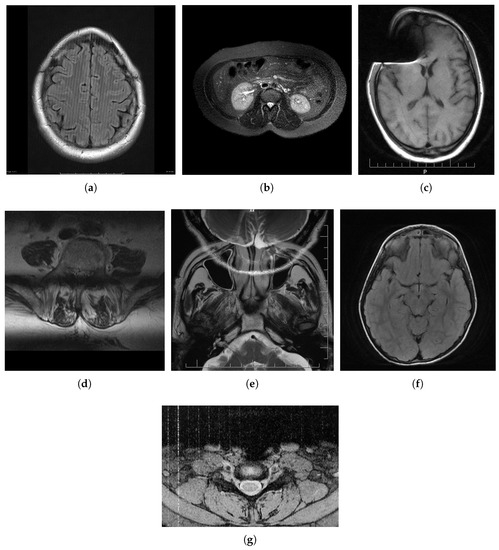
\includegraphics[width=.7\textwidth]{imagenes/chapter2/MedicalDistortions}
  \caption[Ejemplo de artefactos sobre imágenes DICOM.]{Ejemplo de artefactos sobre imágenes médicas~\cite{MoreMedicalDistortion}: 
     (a) \emph{herringbone}, (b) \emph{ghosting}, (c) susceptibilidad magnética, (d) superposición de cortes, (e) \emph{aliasing}, (f) efecto de Gibbs, y (g) \emph{zipper}.
   }
  \label{fig:DicomDistortionsExample}
\end{figure}

En la Figura \ref{fig:DicomDistortionsExample} se aprecian las siguientes distorsiones:
\begin{description}
  \item[(a)] \textbf{\emph{Herringbone}}: causa variaciones en intensidad y superposición 
    de bandas oscuras en imágenes debido a la transformada de Fourier.
  \item[(b)] \textbf{\emph{Ghosting}}: influenciado por reacciones físicas del paciente, 
    factores ambientales y movimientos pulsátiles, como latidos cardíacos, 
    puede causar distorsiones que se superponen con la imagen.
  \item[(c)] \textbf{Susceptibilidad magnética}: al ubicar tejidos en un campo magnético, 
    su magnetización desigual debido a la susceptibilidad magnética causa 
    distorsiones geométricas y variaciones de señal, acentuadas por implantes 
    metálicos altamente susceptibles.
  \item[(d)] \textbf{Superposición de cortes}: pérdida de señal visible en la imagen 
    debido a la adquisición desde múltiples ángulos. 
    En esta distorsión, las secciones en los bordes tienen una intensidad de señal 
    reducida y no crean un perfil de corte con bordes rectos.
  \item[(e)] \textbf{\emph{Aliasing}}: Los artefactos de aliasing surgen cuando el campo 
    de visión es menor que la zona corporal capturada, generando superposición 
    de estructuras regulares. En imágenes médicas, estas distorsiones pueden 
    aparecer como un patrón de franjas o líneas que no corresponden 
    correctamente a la anatomía real.
  \item[(f)] \textbf{Efecto de Gibbs}: también conocidos como artefactos de truncamiento 
    o artefactos de anillos, son una serie de líneas en la imagen de resonancia 
    magnética que aparecen paralelas al área donde ha ocurrido un cambio repentino 
    e intenso en la intensidad de la señal.
  \item[(g)] \textbf{\emph{Zipper}}: área de píxeles alternantes claros y oscuros, presente en la dirección de codificación de frecuencia y que aparece en toda la serie de imágenes.
\end{description}
La mayoría de estas distorsiones, y combinaciones de ellas, no ocurren de forma natural 
en las imágenes habituales del problema IQA. Como consecuencia, es necesario diseñar 
adaptaciones de los modelos actuales y, por lo tanto, el número de métodos médicos 
existentes se reduce, con ninguno, al momento de escritura, aplicado directamente a la reconstrucción 3D. 
Dichas reconstrucciones suelen ser nubes de puntos~\cite{WhyUsePointCloud}. 

Las nubes de puntos o conjunto de puntos arbitrarios extraídos de la superficie 
de un objeto de interés es uno de las representaciones más comunes y flexibles:
los objetos representados ya sea mediante volúmenes de vóxeles o mallas poligonales
pueden muestrearse fácilmente en nubes de puntos. Además, la adquisición de 
datos a través de escaneo, segmentación u obtenidos de algoritmos de reconstrucción 
3D generalmente proporcionan información geométrica en forma de un conjunto de puntos. 
Las superficies reconstruidas pueden ser aplicadas para:
medición morfológica para el grosor de la corteza o los huesos,
extracción de la línea central (esqueleto de curva) para traqueotomía o colonoscopía,
particionamiento de superficies para clasificación de superficies corticales o
anatómicas, así como registro y correspondencia de formas de tumores o huesos carpales 
\cite{WhyUsePointCloud}.

Es por ello que se propone investigar específicamente el uso de métodos tridimensionales
para el ámbito biomédico, aplicado a las reconstrucciones y visualizaciones volumétricas 
que se suelen emplear en medicina. Todo el desarrollo del proyecto se puede 
ver en el GitHub \url{https://github.com/CodeBoy-source/TFG_NRPCQA}.

\section{Motivación}
 
En el caso del ámbito biomédico, dados los rápidos avances 
de las técnicas no invasivas y la gran cantidad de fabricantes 
de equipamientos, nació el estándar \emph{DICOM}~\cite{Parisot1995} en 1995 
con el objeto de hacer que el intercambio de imágenes médicas se realizase de forma 
fácil, segura y con alta calidad. Este estándar pretendía permitir la integración con diversos sistemas, 
almacenar información extra en forma de metadatos y anotaciones, así como segmentaciones que facilitasen la reconstrucción 3D de diferentes regiones anatómicas.

Cada vez más frecuentemente se emplean volúmenes tridimensionales, como tomografías computarizadas o
resonancias magnéticas en lugar de radiografías convencionales, porque 
proporcionan una visión más completa y detallada de la anatomía y las estructuras 
internas del cuerpo (véase Figura \ref{fig:SlicerVisualization}). 
Esta visualización tridimensional permite a los médicos y personal sanitario 
identificar con mayor precisión lesiones, enfermedades o anormalidades,
así como facilitar la planificación quirúrgica, entre otros~\cite{3DImagingInMedicine, 3DImagingInMedicine2, ADAS3D}.
 
\begin{figure}[htp]
  \begin{center}
    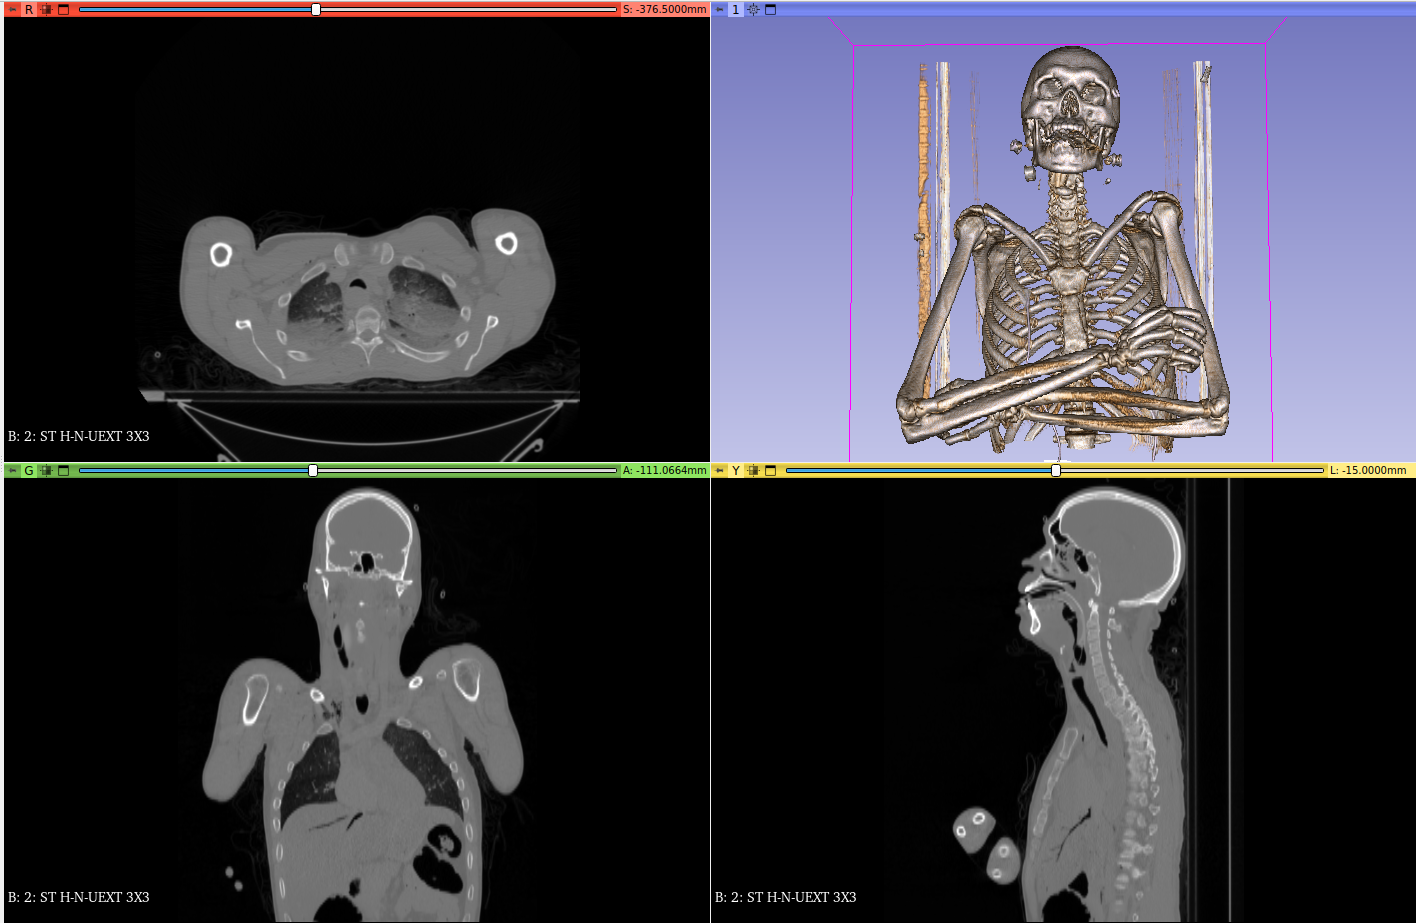
\includegraphics[width=0.8\textwidth]{imagenes/chapter1/SlicerVisualization}
  \end{center}
  \caption[Ejemplo de visualización de un directorio DICOM.]{Ejemplo de visualización de un directorio \emph{DICOM}
    empleando \emph{Slicer3D}~\cite{Slicer3D}. Se pueden observar
  las proyecciones axial (arriba izquierda), coronal (abajo izquierda),
  y sagital (abajo derecha). También se muestra una renderización volumétrica
de los huesos (arriba derecha).
} 
  \label{fig:SlicerVisualization}
\end{figure}

No obstante, cabe mencionar que las distorsiones
están muy presentes en las imágenes médicas~\cite{MedicalImpactOfDistortions}, 
prevaleciendo las distorsiones de contraste, ruido y difuminado\footnote{
  Con \emph{ruido} nos referimos a pequeñas fluctuaciones no deseadas en los colores
  debido a interferencias de todo tipo. \emph{Difuminado} se refiere a la 
  pérdida de detalles en los bordes.
}, 
que se detallarán en la Sección \ref{sec:Distorsiones}.
Estas, a su vez, podrían afectar al volumen 3D que se puede generar a partir 
las imágenes médicas, influyendo en el análisis y diagnóstico asociados. Por ejemplo, 
 en~\cite{XrayRejectionFactor} se estudiaron las razones por las que se suelen 
rechazar las radiografías y su relación relación con el diagnóstico final. 
Reveló que la mayoría de los rechazos se producen por 
errores de posicionamiento, valores inadecuados de exposición, artefactos 
y los problemas de cooperación del paciente. 
Además, no es difícil imaginar que una alta 
calidad de imagen médica tiene implicaciones significativas sobre el cuidado
del paciente. Ya que la mala calidad de imagen puede provocar diagnósticos erróneos. 
Sin mencionar los elevados costes que supone realizar 
nuevas pruebas para conciliar las anteriores. 

Por todo ello, las contribuciones relativas al IQA en el 
ámbito biomédico son claramente bienvenidas, resultando en 
una potencial reducción de costes (menos pruebas), de tiempo de consulta, y mejora 
en la calidad del diagnóstico médico. 

\section{Objetivos}
El objetivo principal de este Trabajo de Fin de Grado (TFG) 
consiste en desarrollar un \textbf{método adecuado para abordar al 
problema de la estimación de la calidad de imágenes médicas tridimensionales}. 
Este objetivo se puede descomponer en una serie de metas parciales: 
\begin{enumerate}
  \item Realizar una revisión exhaustiva del estado del arte para la estimación de calidad 
    de imágenes 3D, así como de la calidad de imágenes médicas 3D en particular.
  \item Estudiar las distorsiones de imagen más comunes, en general, y analizar los patrones de distorsión que afectan la calidad de las imágenes 
    biomédicas.
  \item Analizar pausadamente los enfoques de inteligencia artificial más prometedores que permitan abordar el problema planteado. 
  \item Generar un conjunto de datos sintético que permita validar 
    los métodos empleados. Para ello, será necesario estudiar diferentes 
    estrategias y métricas de evaluación objetivas.
  \item Realizar un estudio experimental que permita validar los enfoques 
    propuestos y extraer conclusiones sobre su aplicabilidad al problema. 
\end{enumerate}

\begin{figure}
  \begin{center}
    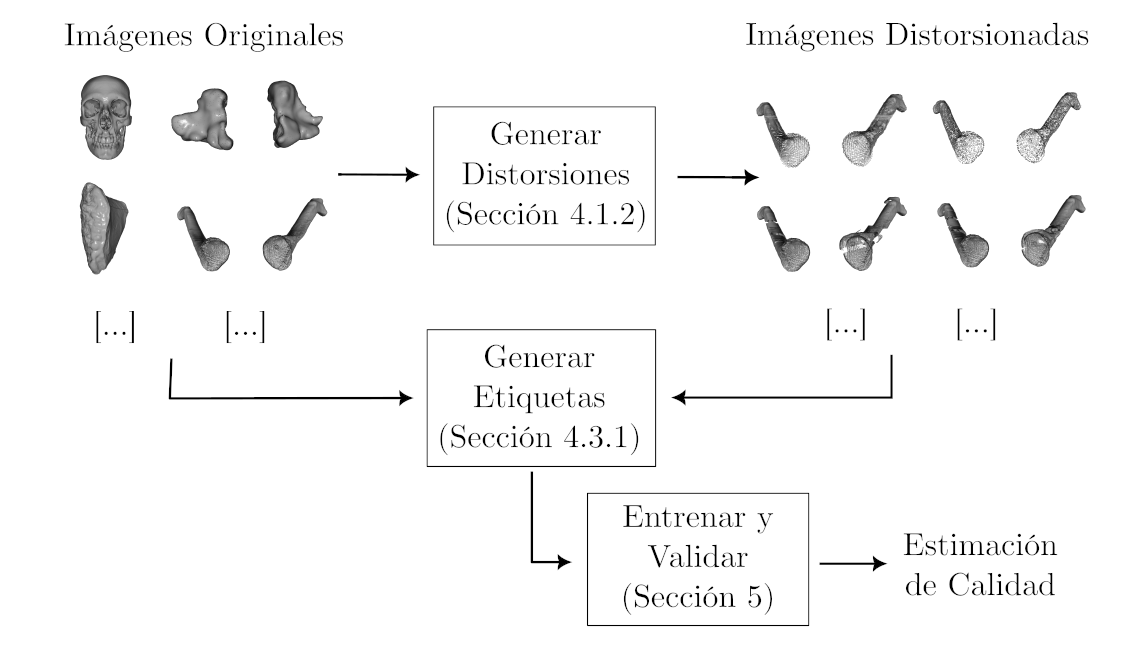
\includegraphics[width=\textwidth]{imagenes/chapter1/Objetivos}
  \end{center}
  \caption{Objetivos de este proyecto.}
  \label{fig:Objetivos}
\end{figure}


\section{Planificación del proyecto}
Al planificar el proyecto, es fundamental tener en cuenta que el TFG 
tiene una carga de 12 créditos ECTS, donde cada 
crédito representa aproximadamente 25 horas de trabajo. 
En total, se estima que se necesitarán alrededor de 300 horas para llevar a cabo 
el proyecto. Considerando que el segundo cuatrimestre tiene aproximadamente 20 semanas, 
se requerirá dedicar al TFG unas 15 horas por semana, lo cual equivaldría a unas 3 horas 
diarias durante 5 días a la semana.
 
La naturaleza del proyecto no presenta una complejidad significativa en términos 
de su alcance y requisitos, lo cual permite abordar su desarrollo a través de un 
enfoque de ciclo de vida en cascada~\cite{ModeloEnCascada}. 
No obstante, bajo este enfoque se evita retroceder en cualquiera de las fases 
del ciclo, y aunque se espera que el diseño y los requisitos del sistema sean 
estables, existe la posibilidad de realizar ajustes menores conforme se obtenga
más información sobre el problema y los métodos. 
Es por ello que utilizamos una pequeña variante, la versión con retroalimentación.
 
Las fases del ciclo de vida son: 
\begin{itemize}
  \item Análisis de requisitos: Consiste en reuniones iniciales con los clientes, 
    en este caso sería los directores del TFG. Se organiza el análisis bibliográfico 
    del problema \emph{IQA} y \emph{PCQA}\footnotemark[4], teniendo en cuenta un estudio previo 
    de las distorsiones médicas.
  \item Diseño: Consistió en la investigación y selección de métodos conforme 
    al análisis anterior, tanto para la resolución como la validación de la solución. 
    Así como pruebas preliminares y diseño del software de experimentación. 
  \item Implementación: Consiste en la adaptación de las técnicas encontradas, 
    implementación de nuevas funcionalidades y generación de un conjunto de datos 
    médicos.
  \item Pruebas: Realización de diversos experimentos de validación, tanto al 
    la generación de las distorsiones como a los modelos y resultados.
\end{itemize}
\footnotetext[4]{\emph{Point cloud quality assessment} o estimación de calidad 
de nubes de puntos} 
\begin{table}[htp]
\centering
\resizebox{\textwidth}{!}{%
\begin{tabular}{|c|c|ll|llll|llll|lllll|llll|llll|}
\hline
\rowcolor[HTML]{FFC702} 
\cellcolor[HTML]{FFC702} & \cellcolor[HTML]{FFC702} & \multicolumn{2}{c|}{\cellcolor[HTML]{FFC702}\textbf{Febrero}} & \multicolumn{4}{c|}{\cellcolor[HTML]{FFC702}\textbf{Marzo}} & \multicolumn{4}{c|}{\cellcolor[HTML]{FFC702}\textbf{Abril}} & \multicolumn{5}{c|}{\cellcolor[HTML]{FFC702}\textbf{Mayo}} & \multicolumn{4}{c|}{\cellcolor[HTML]{FFC702}\textbf{Junio}} & \multicolumn{4}{c|}{\cellcolor[HTML]{FFC702}\textbf{Julio}} \\ \cline{3-25} 
\rowcolor[HTML]{FFC702} 
\multirow{-2}{*}{\cellcolor[HTML]{FFC702}\textbf{Tarea}} & \multirow{-2}{*}{\cellcolor[HTML]{FFC702}\begin{tabular}[c]{@{}c@{}}\textbf{Semanas -}\\ \textbf{Horas}\end{tabular}} & \multicolumn{1}{c}{\cellcolor[HTML]{FFC702}21} & \multicolumn{1}{c|}{\cellcolor[HTML]{FFC702}28} & \multicolumn{1}{c}{\cellcolor[HTML]{FFC702}07} & \multicolumn{1}{c}{\cellcolor[HTML]{FFC702}14} & \multicolumn{1}{c}{\cellcolor[HTML]{FFC702}21} & \multicolumn{1}{c|}{\cellcolor[HTML]{FFC702}28} & \multicolumn{1}{c}{\cellcolor[HTML]{FFC702}04} & \multicolumn{1}{c}{\cellcolor[HTML]{FFC702}11} & \multicolumn{1}{c}{\cellcolor[HTML]{FFC702}18} & \multicolumn{1}{c|}{\cellcolor[HTML]{FFC702}25} & \multicolumn{1}{c}{\cellcolor[HTML]{FFC702}02} & \multicolumn{1}{c}{\cellcolor[HTML]{FFC702}09} & \multicolumn{1}{c}{\cellcolor[HTML]{FFC702}16} & \multicolumn{1}{c}{\cellcolor[HTML]{FFC702}23} & \multicolumn{1}{c|}{\cellcolor[HTML]{FFC702}30} & \multicolumn{1}{c}{\cellcolor[HTML]{FFC702}06} & \multicolumn{1}{c}{\cellcolor[HTML]{FFC702}13} & \multicolumn{1}{c}{\cellcolor[HTML]{FFC702}20} & \multicolumn{1}{c|}{\cellcolor[HTML]{FFC702}27} & \multicolumn{1}{c}{\cellcolor[HTML]{FFC702}04} & \multicolumn{1}{c}{\cellcolor[HTML]{FFC702}11} & \multicolumn{1}{c}{\cellcolor[HTML]{FFC702}18} & \multicolumn{1}{c|}{\cellcolor[HTML]{FFC702}25} \\ \hline
Análisis de Requisitos & 4 - 60 & \cellcolor[HTML]{9B9B9B} & \cellcolor[HTML]{9B9B9B} & \cellcolor[HTML]{9B9B9B} & \cellcolor[HTML]{9B9B9B} & \cellcolor[HTML]{9B9B9B} &  &  &  &  &  &  &  &  &  &  &  &  &  &  &  &  &  &  \\ \cline{1-1}
Diseño & 4 - 60 &  &  &  &  & & \cellcolor[HTML]{9B9B9B} & \cellcolor[HTML]{9B9B9B} & \cellcolor[HTML]{9B9B9B} & \cellcolor[HTML]{9B9B9B}  & \cellcolor[HTML]{9B9B9B} &  &  &  &  &  &  &  &  &  &  &  &  &  \\ \cline{1-1}
Implementación & 6 - 90 &  &  &  &  &  &  &  &  & & & \cellcolor[HTML]{9B9B9B} & \cellcolor[HTML]{9B9B9B} & \cellcolor[HTML]{9B9B9B} & \cellcolor[HTML]{9B9B9B} & \cellcolor[HTML]{9B9B9B} &  &  &  &  &  &  &  &  \\ \cline{1-1}
Pruebas & 6 - 90 &  &  &  &  &  &  &  &  &  &  &  &  &  &  & & \cellcolor[HTML]{9B9B9B} & \cellcolor[HTML]{9B9B9B} & \cellcolor[HTML]{9B9B9B} & \cellcolor[HTML]{9B9B9B} & &  &  &  \\ \hline
\end{tabular}%
}
\caption{Planificación temporal inicial del proyecto.}
\label{tab:PlanificacionTemporal}
\end{table}

La planificación inicial se muestra en la Tabla \ref{tab:PlanificacionTemporal}. 
Dicha planificación sufrió ciertos retrasos debido a que el alumno estaba realizando prácticas de empresa, tenía 
una asignatura y participaba de un curso de \emph{Google} ofrecido por la universidad.
Además, se esperaba que ocurrieran retrasos, sobre todo en la implementación, 
como se puede ver en la Tabla \ref{tab:PlanificacionFinal}, dada la novedad de la propuesta
y la dificultad del problema. En concreto, por ejemplo, el hecho de simular las distorsiones 
médicas fue un proceso iterativo y manual que llevó más tiempo de lo esperado. 

\begin{table}[H]
\resizebox{\textwidth}{!}{%
\begin{tabular}{|c|c|ll|llll|llll|lllll|llll|llll|}
\hline
\rowcolor[HTML]{FFC702} 
\cellcolor[HTML]{FFC702} & \cellcolor[HTML]{FFC702} & \multicolumn{2}{c|}{\cellcolor[HTML]{FFC702}\textbf{Febrero}} & \multicolumn{4}{c|}{\cellcolor[HTML]{FFC702}\textbf{Marzo}} & \multicolumn{4}{c|}{\cellcolor[HTML]{FFC702}\textbf{Abril}} & \multicolumn{5}{c|}{\cellcolor[HTML]{FFC702}\textbf{Mayo}} & \multicolumn{4}{c|}{\cellcolor[HTML]{FFC702}\textbf{Junio}} & \multicolumn{4}{c|}{\cellcolor[HTML]{FFC702}\textbf{Julio}} \\ \cline{3-25} 
\rowcolor[HTML]{FFC702} 
\multirow{-2}{*}{\cellcolor[HTML]{FFC702}\textbf{Tarea}} & \multirow{-2}{*}{\cellcolor[HTML]{FFC702}\begin{tabular}[c]{@{}c@{}}\textbf{Semanas -}\\ \textbf{Horas}\end{tabular}} & \multicolumn{1}{c}{\cellcolor[HTML]{FFC702}21} & \multicolumn{1}{c|}{\cellcolor[HTML]{FFC702}28} & \multicolumn{1}{c}{\cellcolor[HTML]{FFC702}07} & \multicolumn{1}{c}{\cellcolor[HTML]{FFC702}14} & \multicolumn{1}{c}{\cellcolor[HTML]{FFC702}21} & \multicolumn{1}{c|}{\cellcolor[HTML]{FFC702}28} & \multicolumn{1}{c}{\cellcolor[HTML]{FFC702}04} & \multicolumn{1}{c}{\cellcolor[HTML]{FFC702}11} & \multicolumn{1}{c}{\cellcolor[HTML]{FFC702}18} & \multicolumn{1}{c|}{\cellcolor[HTML]{FFC702}25} & \multicolumn{1}{c}{\cellcolor[HTML]{FFC702}02} & \multicolumn{1}{c}{\cellcolor[HTML]{FFC702}09} & \multicolumn{1}{c}{\cellcolor[HTML]{FFC702}16} & \multicolumn{1}{c}{\cellcolor[HTML]{FFC702}23} & \multicolumn{1}{c|}{\cellcolor[HTML]{FFC702}30} & \multicolumn{1}{c}{\cellcolor[HTML]{FFC702}06} & \multicolumn{1}{c}{\cellcolor[HTML]{FFC702}13} & \multicolumn{1}{c}{\cellcolor[HTML]{FFC702}20} & \multicolumn{1}{c|}{\cellcolor[HTML]{FFC702}27} & \multicolumn{1}{c}{\cellcolor[HTML]{FFC702}04} & \multicolumn{1}{c}{\cellcolor[HTML]{FFC702}11} & \multicolumn{1}{c}{\cellcolor[HTML]{FFC702}18} & \multicolumn{1}{c|}{\cellcolor[HTML]{FFC702}25} \\ \hline
Análisis de Requisitos & 5 - 75 & \cellcolor[HTML]{9B9B9B} & \cellcolor[HTML]{9B9B9B} & \cellcolor[HTML]{9B9B9B} & \cellcolor[HTML]{9B9B9B} & &  &  &  &  &  &  &  &  &  &  &  &  &  &  &  &  &  &  \\ \cline{1-1}
Diseño & 4 - 60 &  &  &  &  & \cellcolor[HTML]{9B9B9B} & \cellcolor[HTML]{9B9B9B} & \cellcolor[HTML]{9B9B9B} & \cellcolor[HTML]{9B9B9B} & &  &  &  &  &  &  &  &  &  &  &  &  &  &  \\ \cline{1-1}
Implementación & 8 - 120 &  &  &  &  &  &  &  &  &  \cellcolor[HTML]{9B9B9B} & \cellcolor[HTML]{9B9B9B} & \cellcolor[HTML]{9B9B9B} & \cellcolor[HTML]{9B9B9B} & &  & \cellcolor[HTML]{9B9B9B}  & \cellcolor[HTML]{9B9B9B}  & & & \cellcolor[HTML]{9B9B9B} & \cellcolor[HTML]{9B9B9B} &  &  &  \\ \cline{1-1}
Pruebas & 6 - 90 &  &  &  &  &  &  &  &  &  &  &  &  & \cellcolor[HTML]{9B9B9B}   & \cellcolor[HTML]{9B9B9B} & & & \cellcolor[HTML]{9B9B9B} & \cellcolor[HTML]{9B9B9B} &  &  & \cellcolor[HTML]{9B9B9B} & \cellcolor[HTML]{9B9B9B} & \\ \hline
\end{tabular}%
}
\caption{Planificación resultante del proyecto.}
\label{tab:PlanificacionFinal}
\end{table}

Para realizar este proyecto se tuvo en cuenta los siguientes materiales:
suscripción a \emph{Google Colab Pro}, un portátil personal de gama media, 
\emph{Google Drive 100GB} y otros gastos. 
Además, para el coste estimado, se asume un salario de 25\officialeuro/hora, como para un investigador \emph{senior} o
responsable I+D de una empresa tecnológica en España. 
 
Respecto al servidor GPU, con las especificaciones actuales de \emph{Google}, 
se estima un coste aproximado de 10.000\officialeuro. Se asume una amortización de 2 años, 
lo que implica un pago diario de 13.70\officialeuro. El desglose total de los costes 
se puede ver en la siguiente Tabla \ref{tab:TotalGastos}.

\begin{table}[H]
\centering
\begin{tabular}{ll}
\hline
\multicolumn{1}{|l|}{\cellcolor[HTML]{FFCB2F}{\textbf{Fecha inicio}}} & \multicolumn{1}{l|}{21/02/2022} \\ \hline
\multicolumn{1}{|l|}{\cellcolor[HTML]{FFCB2F}{\textbf{Fecha fin}}} & \multicolumn{1}{l|}{25/07/2022} \\ \hline
\multicolumn{1}{|l|}{\cellcolor[HTML]{FFCB2F}{\textbf{Duración}}} & \multicolumn{1}{l|}{154 días, 110 laborables} \\ \hline
\textbf{} & 
\end{tabular}
\caption{Total de horas y días trabajados.}
\label{tab:TotalTrabajado}
\end{table}

\begin{table}[H] 
  \centering
  \begin{tabular}{ll}
\hline
\rowcolor[HTML]{FFCB2F} 
\multicolumn{1}{|c|}{\cellcolor[HTML]{FFCB2F}{\textbf{Item}}} & \multicolumn{1}{c|}{\cellcolor[HTML]{FFCB2F}{\textbf{Costo}}} \\ \hline
\multicolumn{1}{|l|}{Salario} & \multicolumn{1}{l|}{8 250.00\officialeuro} \\ \hline
\multicolumn{1}{|l|}{Portátil de Gama Media} & \multicolumn{1}{l|}{700.00\officialeuro} \\ \hline
\multicolumn{1}{|l|}{Google Colab Pro} & \multicolumn{1}{l|}{55.50\officialeuro} \\ \hline
\multicolumn{1}{|l|}{Servidor GPU} & \multicolumn{1}{l|}{2 109.8\officialeuro} \\ \hline
\multicolumn{1}{|l|}{Google Drive 100GB} & \multicolumn{1}{l|}{10.00\officialeuro} \\ \hline
\multicolumn{1}{|l|}{Otros} & \multicolumn{1}{l|}{300.00\officialeuro} \\ \hline
\multicolumn{1}{|r|}{\cellcolor[HTML]{FFCB2F}{\textbf{Total}}} & \multicolumn{1}{l|}{ 11.425,3 \officialeuro} \\ \hline
\textbf{} & 
\end{tabular}
\caption{Estimación final de coste del proyecto.}
\label{tab:TotalGastos}
\end{table}

%
\chapter{Fundamentos Teóricos}
\section{Image Quality Assessment (IQA)}
\label{sec:IQA}
Existen tres subproblemas presenten en el ámbito de \emph{IQA}. Los primeros, son problemas 
donde tenemos acceso a la imagen original, que suponemos exenta de desperfectos, 
en la cual se pueden aplicar métodos basados en diferencia de características 
entre ambas, como puede ser al nivel del color de píxel posición a posición,
y se denomina ``\emph{Full Reference}''(\emph{FR}). 
La tarea, aparentemente sencilla, en realidad presenta una complejidad alta dada por 
la necesidad de codificar la percepción humana a la hora de calificar la calidad 
de una imagen~\cite{WhyIsIQASoDifficult}, ya que métricas que miden distancias no suelen 
ser suficientes al no haber buena correlación entre la calidad percibida y el 
resultado de la métrica.

La mayoría de las veces no se menciona, pero al optar métodos de sensibilidad 
al error (distancias) se imponen un conjunto de suposiciones cuestionables. 
Primeramente, se asume la misma importancia para todas las señales de la imagen\footnote{
  Con \emph{señales} nos referimos a los diferentes canales de color RGB.
}, que
la magnitud del error es lo único que determina la calidad, que el contenido de la imagen 
no afecta al resultado final tras aplicar una distorsión, y que si cambiamos el 
orden de las señales la medida de distorsión no es afectada.
Lamentablemente, ninguna de estas suposiciones se cumplen~\cite{Wang2006ModernIQ} (véase Figuras \ref{fig:FailureMinkowskiMetric} y \ref{fig:MSEHyperSphere}, 
que utilizan distancias \emph{Minkowski}\footnotemark[2] y \emph{MSE}\footnotemark[3] respectivamente).

\begin{figure}[htp]
  \begin{center}
    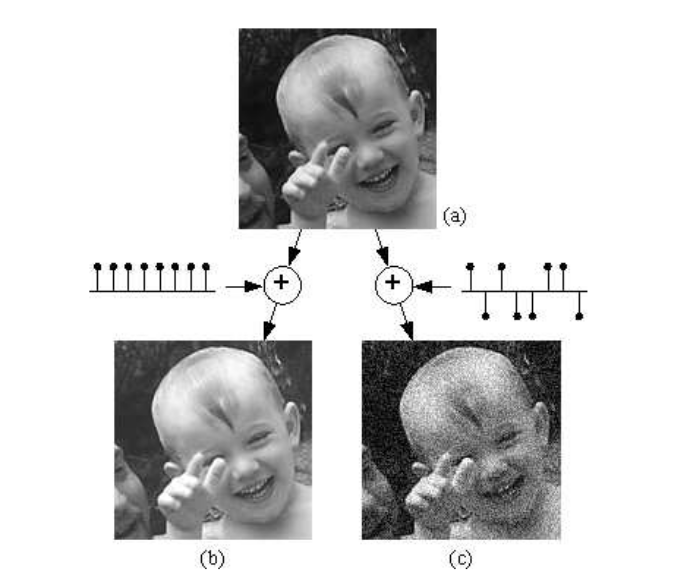
\includegraphics[width=0.6\textwidth]{imagenes/chapter2/failure_minkowski_metric.png}
  \end{center}
  \caption[Visualización del problema de la métrica \emph{Minkowski}.]{En este ejemplo, extraído de~\cite{MinkowskiFailure},
  vemos que sumar una constante positiva a una imagen  de referencia (a) produce la imagen (b) que contiene la misma distancia \emph{Minkowski}
  que (c), imagen fabricada por la misma constante pero permutando signo de forma aleatoria, resultando que
  la percepción final es que la imagen (c) es peor que la imagen (b).
\label{fig:FailureMinkowskiMetric}}
\end{figure}
\begin{figure}[htp]
  \begin{center}
    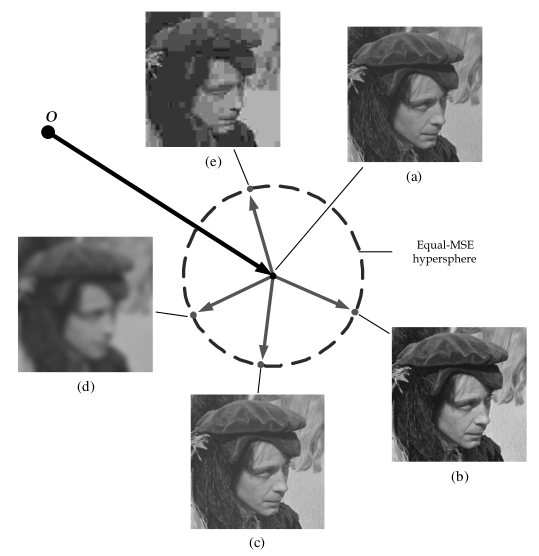
\includegraphics[width=0.6\textwidth]{imagenes/chapter2/MSE_Hypersphere.png}
  \end{center}
  \caption[Visualización del hiperplano MSE de imágenes distorsionadas.]{En este ejemplo, extraído de~\cite{Wang2006ModernIQ}, la misma imagen distorsionada de distintas 
    maneras resulta en la misma distancia, con valor MSE=181. 
    No obstante, es evidente que algunas distorsiones producen efectos visuales más marcados que otras.}
  \label{fig:MSEHyperSphere}
\end{figure}
\footnotetext[2]{La distancia de \emph{Minkowski} es una métrica 
vectorial que puede considerarse como una generalización tanto de 
la distancia euclídea como de la distancia de Manhattan. }
\footnotetext[3]{\emph{Mean squared error} o error cuadrático medio 
  es una métrica de distancia que se calcula como la media de la suma de las 
  diferencias al cuadrado.
} 
 
El siguiente subproblema es aquel donde tenemos algún tipo de información adicional, incompleta, respecto 
a la imagen original el momento de análisis de la calidad de la imagen final,
denominados ``\emph{Reduced Reference}''(\emph{RR}). La información extra puede 
incluir metadatos, parámetros 
de compresión, características estadísticas o extraídas de una región de interés específica.
 
Y por último, tenemos aquellos problemas donde desconocemos el origen y cualquier 
información respecto a la imagen inicial, denominados problemas ``\emph{No reference}''(\emph{NR}).
Estas métricas están exentas de cualquier información de referencia y se 
centran en capturar características generales de calidad.

\begin{figure}[htp]
  \centering
  \begin{subfigure}{0.49\textwidth}
  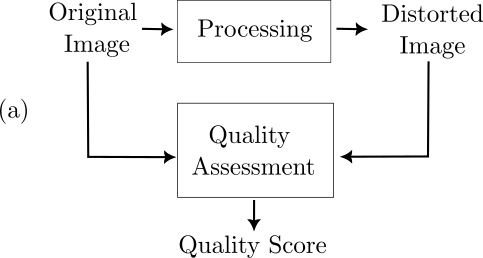
\includegraphics[width=0.95\textwidth]{imagenes/chapter2/FullReferenceInk.png}
  \end{subfigure}
  \begin{subfigure}{0.49\textwidth}
  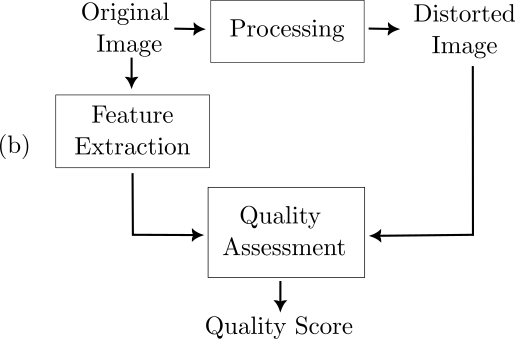
\includegraphics[width=0.95\textwidth]{imagenes/chapter2/ReducedReferenceInk.png}
  \end{subfigure}
  \par\bigskip
  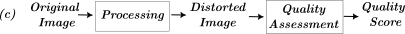
\includegraphics[]{imagenes/chapter2/NoReferenceInk.png}
  \caption{Resumen de subproblemas IQA. La imagen (a) representa el subproblema FR, 
  la imagen (b) RR y la imagen (c) NR.}
  \label{fig:IQASubproblems}
\end{figure}


La evaluación de calidad de imagen sin referencia es, quizás, el problema 
más difícil en el análisis de imágenes. De cierto modo, el modelo debe ser 
capaz de evaluar la calidad de cualquier imagen sin saber nada de la imagen ``real'', original. 
Superficialmente parece ``misión imposible''. No obstante, esa 
es una tarea sorprendentemente sencilla para el ser humano~\cite{Wang2006ModernIQ}. 

Para resolver problemas NR, debemos disponer de conocimientos de la naturaleza de las imágenes 
de las que tratamos y los efectos de las distorsiones. Lo que se denomina 
estadísticas naturales de escena (NSS, por sus siglas en inglés). Un ejemplo 
sería JPEG, un algoritmo de compresión que se codifica por bloques 8x8. Los efectos
negativos de la compresión se representan por el difuminado entre bloques y los artefactos que generan.
Entender estos efectos permite diseñar métricas específicas~\cite{SpatialDomainForJPEG}

As veces resulta difícil describir las características de la imagen y los efectos 
de la distorsión. Es por ello que los métodos de aprendizaje profundo son cada vez 
más frecuente y dan mejores resultados. Permitimos que sea la máquina la que aprenda 
las propiedades de la distorsión, su relación con el contenido y efecto sobre la 
percepción visual~\cite{Hallucinated-IQA, BIQA, DIPIQA}. 

La complejidad del problema crece conforme nos desplazamos a las tres dimensiones. 
El analizar la calidad de los modelos \emph{3D} implica mayor nivel de dificultad 
dado que nos enfrentamos a dos grandes retos: La complejidad computacional 
de las operaciones y la escasez de bases de datos etiquetadas
sobre objetos tridimensionales para entrenar y evaluar modelos. 

Para las nubes de puntos, que representan una colección de puntos en un espacio 
tridimensional $(x,y,z)$ cada uno con un color asociado \emph{RGB}\footnote{
  RGB son las siglas en inglés para rojo, verde y azul. Los colores se representan 
  por tripletas de valores en escala 0-255 ó 0-1 que significan la cantidad que aporta 
  cada color. 
}, se pueden emplear métricas y algoritmos basándose en criterios como la 
densidad de puntos, la uniformidad, la precisión geométrica y la detección de artefactos.
También se pueden considerar aspectos relacionados con la coherencia de los colores 
o texturas asociadas a los puntos~\cite{NR3DQA, StructureGuidedResampling, GPA-NET}.
Un enfoque común es la evaluación de calidad de una nube de puntos tridimensional 
mediante proyecciones \emph{2D} desde diferentes perspectivas~\cite{IT-PCQA, VQA-PC, MM-PCQA}. 
De esta forma podemos tratar el problema como uno de \emph{IQA} 2D reduciendo la 
complejidad computacional, pudiendo implementar métodos y soluciones ya existentes.

Teniendo en cuenta todas estas consideraciones, el presente TFG aborda la
estimación, sin referencia, de calidad de imágenes médicas en espacio tridimensional.



\section{Aprendizaje Automático y Profundo}
\subsection{Aprendizaje Automático}
El aprendizaje automático~\cite{IAModernApproach} o \emph{Machine Learning} (\emph{ML}) 
es una de las ramas que compone lo que definimos como 
la inteligencia artificial (\emph{IA}). Permite a las computadoras aprender a partir de datos sin programación explícita. 
A través de algoritmos y modelos, pueden reconocer patrones, hacer predicciones y tomar decisiones basadas en información proporcionada.

En este caso hablamos de dar soluciones a problemas complejos sin 
solución analítica (o que resulta muy costoso hallarla), es decir, necesitamos que la computadora sea la que identifique
los patrones en los datos y realice predicciones sobre ellos~\cite{LearningFromData}.
Se puede definir más formalmente que un programa aprende de la experiencia E con
respecto a alguna clase de tareas T y una métrica de rendimiento P si su
rendimiento en las tareas T, medido con P, mejora con la experiencia E~\cite{TomMitchell}.

Dependiendo de factores como las necesidades del problema, la naturaleza
de los datos a utilizar o el objetivo a alcanzar, podemos encontrar distintos tipos de
algoritmos de aprendizaje. En este documento se recogerán dos grandes grupos: aprendizaje supervisado 
y aprendizaje no supervisado. En el primero disponemos de un conjunto de datos 
anotados, es decir, con las salidas deseadas para cada ejemplo y en el segundo 
se espera que sea la máquina la que determine los patrones (véase Figuras \ref{fig:SupervisedExample} y \ref{fig:UnsupervisedExample}). 
En general se suelen aplicar las técnicas de \emph{ML} sobre grandes conjuntos 
de datos sobre los cuales deseamos detectar los patrones subyacentes~\cite{
DataMiningHandbook}.

Puede observarse que dadas estas descripciones, el problema presente puede ser 
abordados mediante técnicas de \emph{ML}: Tenemos datos de entrada (características 
extraídas de nubes de puntos distorsionadas) y una salida (valor de calidad). Además, existen conjuntos de 
datos públicos etiquetadas para distintos tipos de distorsiones. Así,
estamos ante un problema de aprendizaje supervisado.

\begin{figure}[htp]
  \centering
    \begin{subfigure}{.3\textwidth}
  \centering
  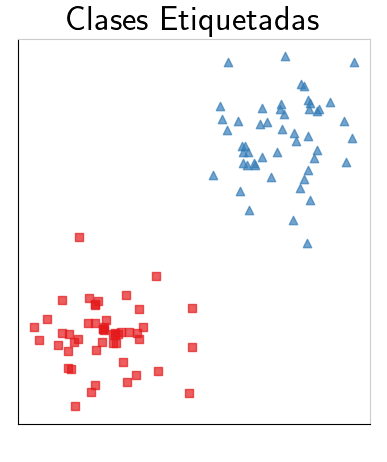
\includegraphics[width=0.8\linewidth]{imagenes/chapter2/BeforeSVMExample.png} 
  \tikz[remember picture]\node[inner sep=0pt,outer sep=0pt] (a) {}; 
    \end{subfigure}
    \begin{subfigure}{.3\textwidth} 
  \centering
  \tikz[remember picture]\node[inner sep=0pt,outer sep=0pt] (b) {}; 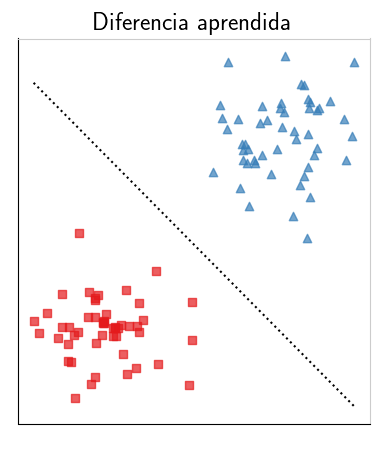
\includegraphics[width=0.8\linewidth]{imagenes/chapter2/AfterSVMExample.png}
    \end{subfigure}
  \tikz[remember picture,overlay]\draw[line width=1pt,-stealth,black] ([xshift=2mm,yshift=2cm]a.east) -- ([xshift=-2mm, yshift=2cm]b.west)node[midway,above,text=black,font=\LARGE\bfseries\sffamily] {};
  \caption[Ejemplo de aprendizaje supervisado.]{
  Ejemplo de aprendizaje supervisado. Vemos como a partir de un conjunto de clases etiquetadas aprendemos un hiper plano que 
  las separa. 
  }
  \label{fig:SupervisedExample}
\end{figure}
\begin{figure}[htp]
  \centering
    \begin{subfigure}{.3\textwidth}
  \centering
  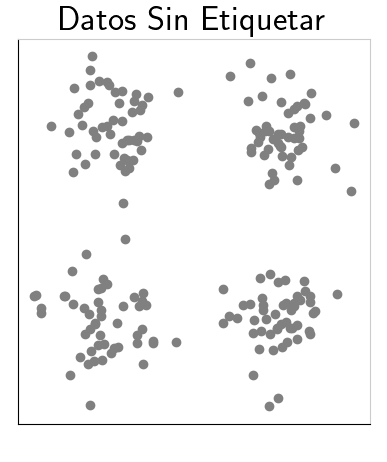
\includegraphics[width=0.8\linewidth]{imagenes/chapter2/BeforeClusteringExample.png} 
  \tikz[remember picture]\node[inner sep=0pt,outer sep=0pt] (c) {}; 
    \end{subfigure}
    \begin{subfigure}{.3\textwidth} 
  \centering
  \tikz[remember picture]\node[inner sep=0pt,outer sep=0pt] (d) {}; 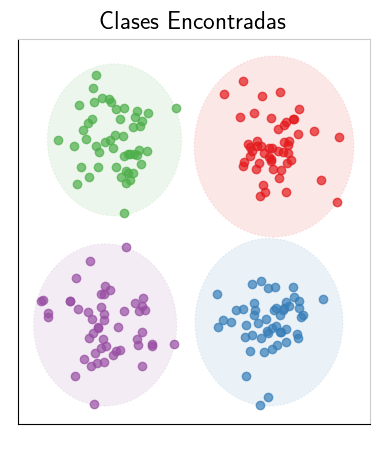
\includegraphics[width=0.8\linewidth]{imagenes/chapter2/AfterClusteringExample.png}
    \end{subfigure}
  \tikz[remember picture,overlay]\draw[line width=1pt,-stealth,black] ([xshift=2mm,yshift=2cm]c.east) -- ([xshift=-2mm, yshift=2cm]d.west)node[midway,above,text=black,font=\LARGE\bfseries\sffamily] {};

  \caption[Ejemplo de aprendizaje no supervisado.]{
  Ejemplo de aprendizaje no supervisado. Dado un conjunto de puntos aprendemos un conjunto de clases 
  a partir de los patrones.
}
  \label{fig:UnsupervisedExample}
\end{figure}

\subsection{Aprendizaje Profundo}
En el aprendizaje profundo o \emph{Deep Learning} (\emph{DL}), 
a diferencia de los modelos anteriores donde tenemos un conjunto de variables 
extraídas por un humano experto, las características sobre la cual inferimos 
son obtenidas por el propio modelo automáticamente~\cite{DeepLMITPress, DeepLearningNature, DeepLearningInNN}.
En términos generales, la extracción automática de características suele 
desempeñar mejores resultados en contra de las características manuales.

La mayoría de los modelos de DL son basados en múltiples capas jerárquicas de 
procesado de datos. Las más conocidas son las redes neuronales (ANN, por sus siglas 
en inglés), modelo bioinspirado que simula el funcionamiento de las neuronas del cerebro
humano (abstracción simplificada)~\cite{ANNForPattern,ANNCambridge}. 

A alto nivel, el funcionamiento de una red neuronal implica tres etapas principales: 
entrada, procesamiento y salida. En la etapa de entrada, se proporciona a la red 
neuronal un conjunto de datos o características que representan la información 
que se desea analizar o procesar. Estos datos de entrada se propagan a través 
de la red neuronal (\emph{feedforward}). En la etapa de procesamiento, las neuronas reciben las entradas 
y realizan cálculos utilizando pesos y funciones de activación. Los pesos representan 
la importancia relativa de las diferentes entradas en el cálculo, y las funciones 
de activación determinan la salida de una neurona en función de su entrada. A medida que los datos se propagan a través de la red neuronal, las capas intermedias 
procesan y combinan las entradas, extrayendo características relevantes y creando 
representaciones internas cada vez más abstractas. Esto permite que la red neuronal aprenda y 
descubra patrones en los datos. Finalmente, en la etapa de salida, la red neuronal 
produce una respuesta o predicción basada en las características extraídas. 
Esto puede ser la clasificación de una imagen, la predicción de un valor numérico o 
cualquier otro resultado deseado. En esta última etapa se calcula el error de 
predicción respecto a la salida deseada con la función de pérdida y se ajusta 
los pesos respectivamente.

El aprendizaje de una red neuronal se logra mediante un proceso llamado entrenamiento.
Donde de forma iterativa repetimos el proceso descrito anteriormente varias veces 
con distintos ejemplos. El conjunto de datos es muy relevante para el correcto 
aprendizaje. Debe de ser representativo, extenso y limpio de anormalidades ya que 
estaremos extrayendo características y relevancias a partir de ellos.

En definitiva, una red neuronal es en esencia una serie de ajustes de parámetros para lograr el resultado deseado. 
Estos incluyen ajuste de los pesos y sesgos iniciales, selección de las funciones de activación, 
como las más utilizadas sigmoide o ReLU, de una función de pérdida y un optimizador, 
encargado de determinar como ajustar los pesos según el error obtenido en cada fase del entrenamiento.
No obstante, existe un fenómeno denominado sobreentrenamiento o \emph{overfitting}. 
Ocurre cuando hay un sobreajuste de los parámetros
hacia los datos de entrenamiento, disminuyendo la capacidad de generalización del modelo. 
Informalmente, es como decir que el modelo ha memorizado los resultados y, por ello, 
con datos nunca vistos posee errores substancialmente altos. Para lidiar con estos 
problemas se deben elegir también formas de regularización del modelo, es decir, 
restricciones sobre el entrenamiento para evitar el sobre ajuste. 

\begin{figure}[htp]
  \centering
  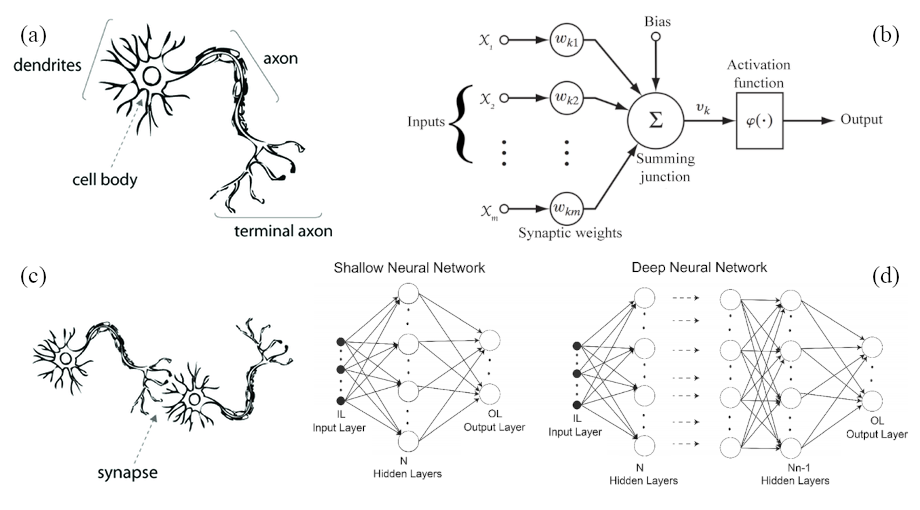
\includegraphics[width=\textwidth]{imagenes/chapter2/ANNVisualization.png}
  \caption[Ejemplo gráfico de una red neuronal.]
  {Ejemplo gráfico de una red neuronal~\cite{NeuronImages, NeuronSimilarity,ShallowAndDeepNN}. 
      En (a) vemos una neurona con su representación artificial simplificada (b). En (c) vemos una conexión entre 
  neuronas y en (d) la representación de diferentes profundidades de conexiones artificiales.}
  \label{fig:ANNVisualization}
\end{figure}

\subsubsection{Redes Convolucionales} 
Las redes convolucionales o \emph{convolutional neural network} (CNN)~\cite{ConvolutionalZipCode, ConvolutionInRadiology}
son un tipo de arquitectura de redes neuronales diseñadas 
específicamente para el procesamiento de datos estructurados en forma de matrices, como imágenes.
Se ha descubierto que son aplicables para el procesado de texto, sonidos y, recientemente,
a superficies tridimensionales.
Utilizan capas convolucionales que aplican filtros a regiones locales de la entrada 
para extraer características relevantes. En la Figura \ref{fig:RadiographyConvolutionExample}
podemos ver un ejemplo de esquema jerárquico de extracción de características para el 
diagnóstico médico a partir de una radiografía. Se puede observar 
que, a diferencia de una ANN, existen dos capas adicionales: capas convolucionales 
y capas de \emph{pooling}.

\begin{figure}[htp]
  \centering
  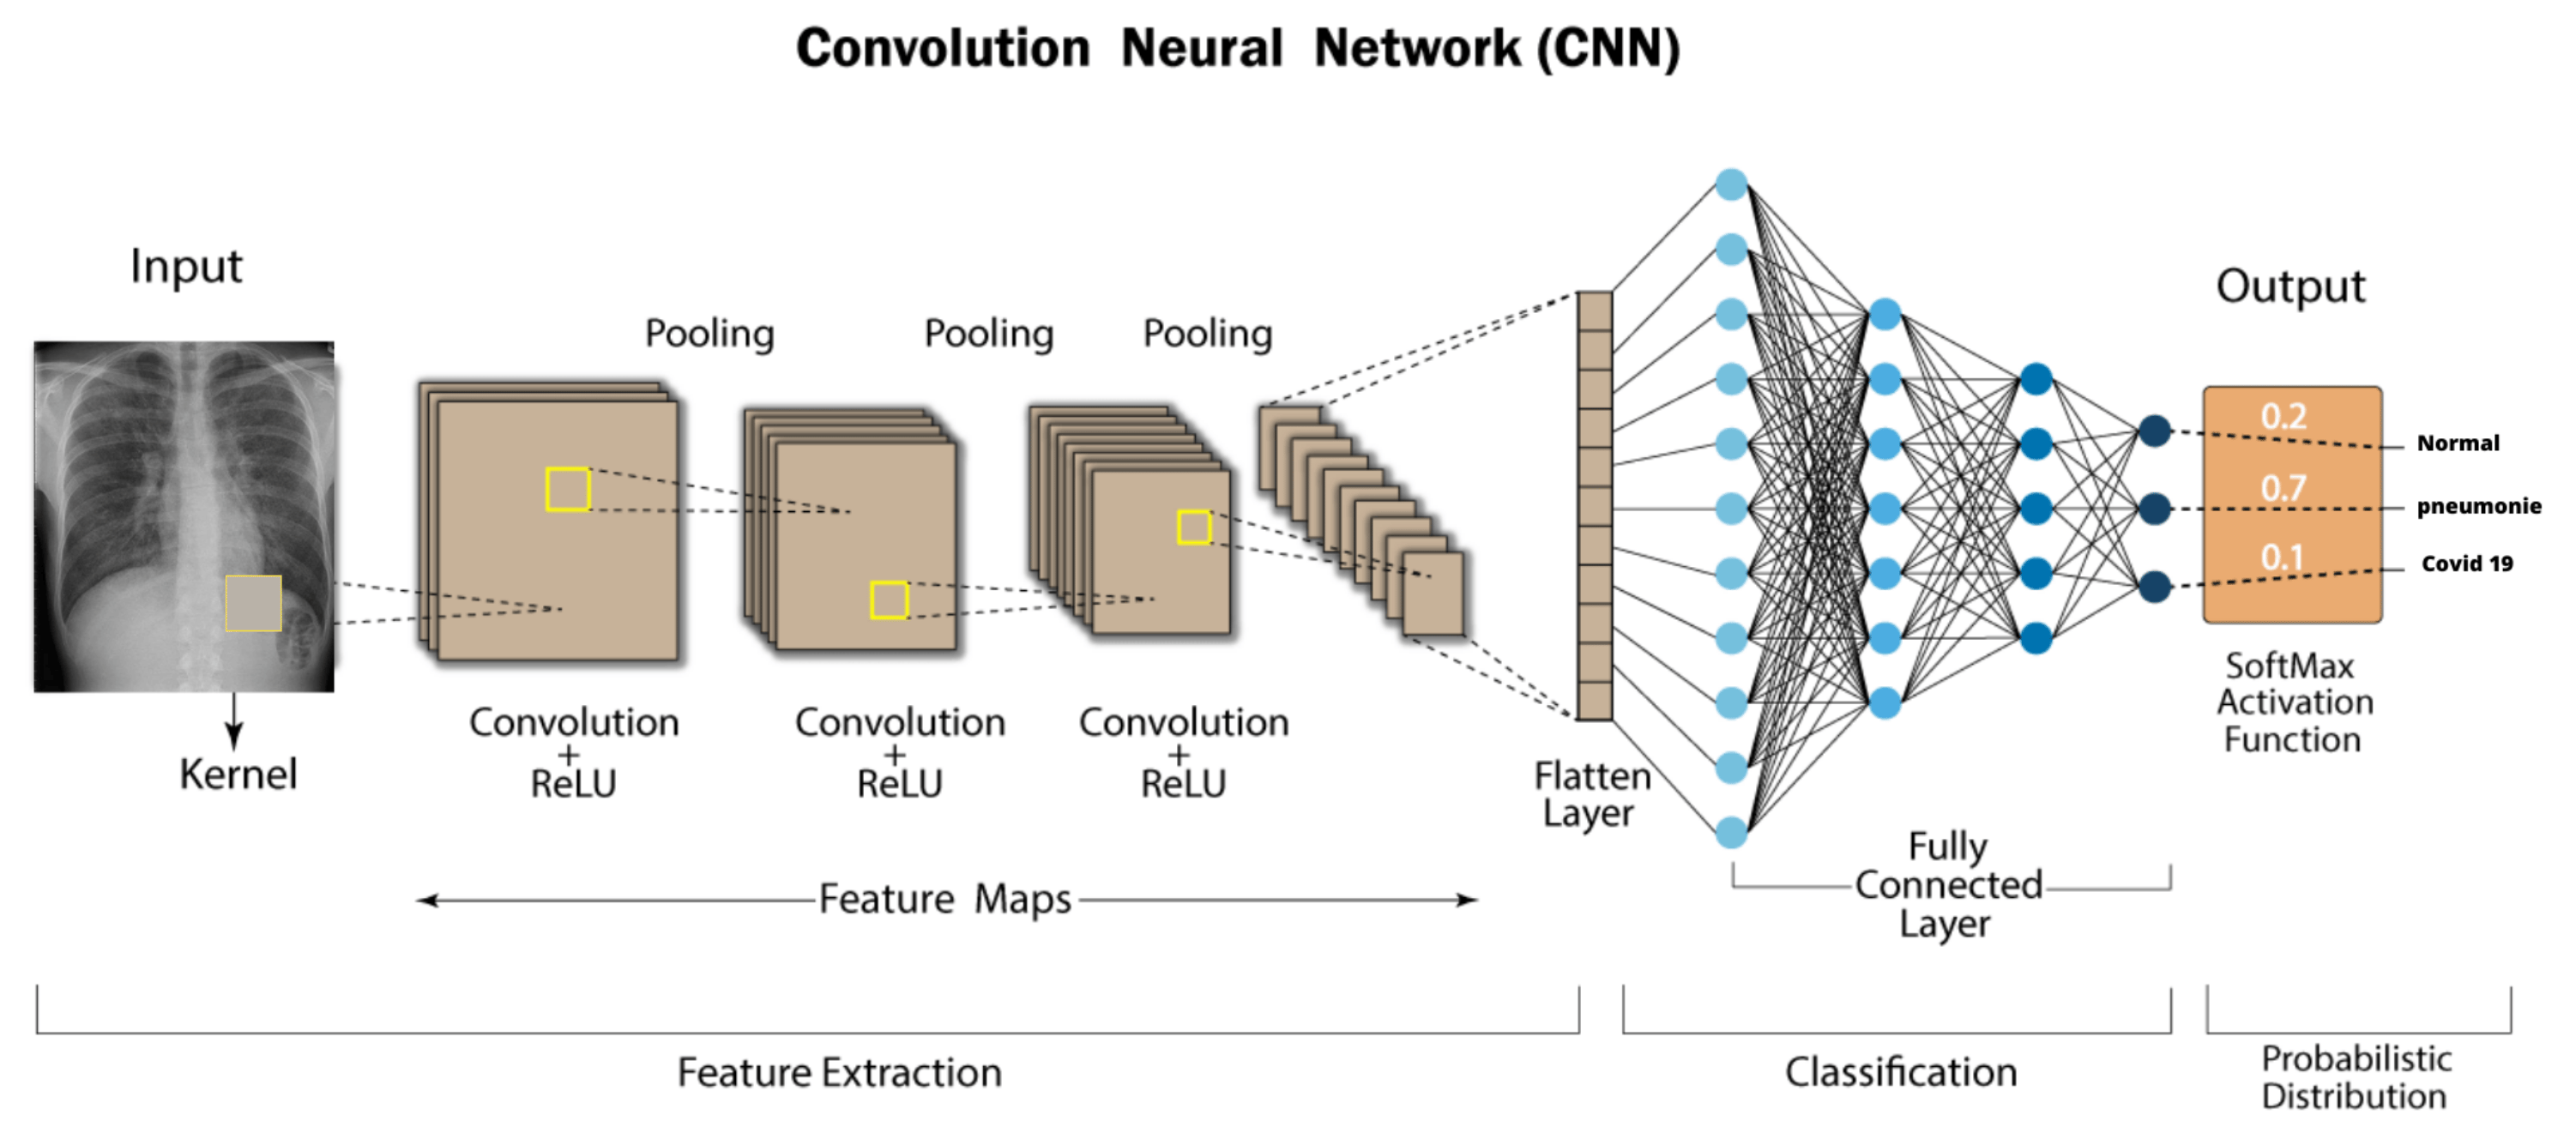
\includegraphics[width=\textwidth]{imagenes/chapter2/RadiographyConvolutionExample.png}
  \caption[Ejemplo de red convolucional para imágenes médicas]{Ejemplo extraída de~\cite{RadiographyConvolutionExample} del proceso de convolución sobre una radiografía pulmonar 
  para la detección de enfermedades.}
  \label{fig:RadiographyConvolutionExample}
\end{figure}

\subsubsection{Capas convolucionales}
Para simplificar la explicación, la realizaremos sobre imágenes 2D. 
Una capa convolucional es encargada de realizar la operación de convolución sobre 
los datos de entrada. 
La convolución se refiere a una operación matemática que combina dos funciones para crear una tercera función.
En este caso, se aplica una operación de convolución 
entre una matriz de entrada (como una imagen) y un filtro (\emph{kernel}).
La operación de convolución implica deslizar el filtro sobre la matriz de entrada, 
multiplicando los elementos coincidentes y sumándolos para obtener un único valor 
en la matriz de salida, conocida como mapa de características. 
Este proceso se repite en diferentes ubicaciones de la matriz de 
entrada para generar el mapa de características completo. En la Figura 
\ref{fig:ConvolutionalRepresentation} vemos una operación sobre la ubicación 
inicial de la imagen, esquina superior izquierda. 
La elección del siguiente trozo 
o \emph{patch} de la imagen suele venir determinado por el paso o \emph{stride}.
Habitualmente se utiliza un \emph{stride} de 1. Es decir, elegimos la matriz 
adyacente con distancia horizontal igual a 1 hasta llegar al final de esa fila 
y luego nos desplazamos 1 hacia abajo. 
Por medio de este proceso, la red es capaz de
capturar dependencias temporales y espaciales en los datos con la aplicación
de los filtros correspondientes.

Podemos observar en la Figura \ref{fig:ConvolutionalRepresentation} que aplicar directamente 
el operador de convolución a una imagen resulta en una reducción del tamaño del mapa 
de activación debido a la naturaleza del operador. 
Sin embargo, esto no siempre es deseable. 
Para abordar este problema, se puede agregar relleno o \emph{padding} a la imagen 
de entrada utilizando información existente en la misma. 
Esto garantiza que el mapa de activación tenga la misma dimensionalidad que 
la imagen original. Además, es posible reducir aún más la salida ajustando 
los saltos o \emph{strides} del filtro de convolución mientras se recorre la imagen.

\begin{figure}[htp]
  \begin{center}
    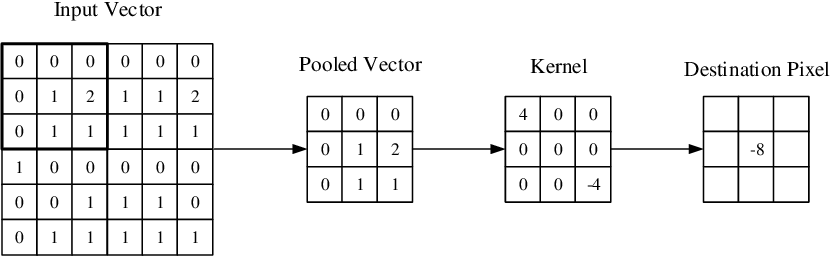
\includegraphics[width=0.95\textwidth]{imagenes/chapter2/ConvolutionalRepresentation.png}
  \end{center}
  \caption[Representación visual de la operación de convolución]{Representación visual de la operación de convolución sobre una imagen, extraída de~\cite{ConvolutionalRepresentation}.
  }
  \label{fig:ConvolutionalRepresentation}
\end{figure}

\subsubsection{Capa de pooling} 
El propósito principal de las capas de \emph{pooling} es reducir la cantidad de parámetros 
y la complejidad computacional de la red, al tiempo que conservan las características 
más relevantes. Además, el \emph{pooling} puede ayudar a hacer que la representación sea 
invariante a pequeñas variaciones en la posición o el tamaño de los objetos en la 
imagen, lo que mejora la capacidad de generalización del modelo.

En la Figura \ref{fig:PoolingExample} vemos un operador de \emph{pooling} común,
el operador de valor máximo. También es habitual el uso del operador de valor medio y
valor mínimo.
El \emph{pooling}, al igual que la convolución, posee un filtro o ventana que recorre
los datos dado un salto o \emph{stride} al moverse por los mismos,

Las capas convolucionales y de \emph{pooling} trabajan en conjunto para procesar y extraer 
características. 
Dependiendo de la complejidad del problema, se puede ajustar el número de estas.

\begin{figure}[htp]
  \begin{center}
    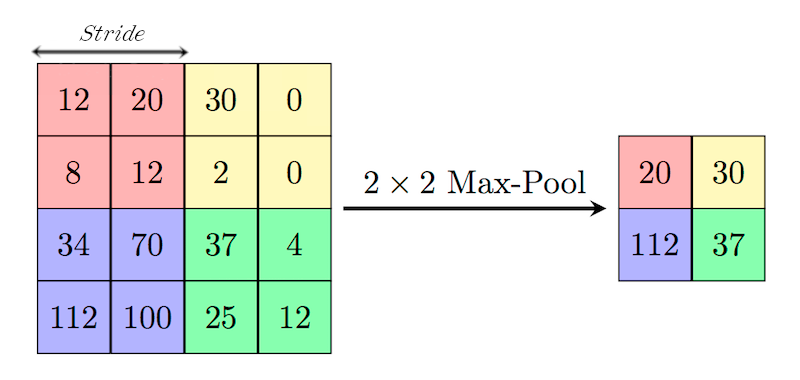
\includegraphics[width=0.65\textwidth]{imagenes/chapter2/MaxpoolSample.png}
  \end{center}

  \caption{
    Ejemplo de operación de \emph{max-pooling} con \emph{stride} a 2.
  }
  \label{fig:PoolingExample}
\end{figure}

\subsubsection{Capas totalmente conectadas}
Las capas totalmente conectadas o \emph{fully connected}, también llamadas 
capas densas o \emph{dense}, son aquellas en las que todas sus neuronas 
están conectadas con todas las neuronas de la capa anterior y de la
siguiente. Si bien existen modelos totalmente convolucionales, resulta común
que las CNN's incluyan capas totalmente conectadas al final de la arquitectura.
Estas capas forman una ANN clásica.
La salida de la última capa densa, siendo la salida de la red entera, es donde
se evaluará la función de pérdida elegida, y al igual que en una red neuronal
clásica se utilizará este valor para ajustar los pesos.

\subsubsection{Aplicadas a Videos} 
\label{sec:VideoCNN}
Las redes convolucionales se pueden llegar a aplicar incluso a videos. 
Para ello, se puede utilizar una variante de las redes convolucionales llamada 
redes convolucionales 3D (3D CNNs) o redes convolucionales espaciotemporales. 
Estas redes están diseñadas específicamente para capturar tanto las características 
espaciales como las temporales presentes en los vídeos.

La principal diferencia entre una red convolucional tradicional y una 3D CNN es 
la adición de una dimensión temporal en las operaciones de convolución. 
En lugar de considerar solo imágenes individuales, se toman secuencias de imágenes 
(\emph{frames}) para capturar la información temporal.

En este TFG se explora el uso de una 3D CNN capaz de analizar vídeos que pertenece 
a la familia que se conoce como \emph{SlowFast networks}~\cite{SlowFastNetworks}. Están basadas en dos caminos 
de entrada de datos. Un conjunto de \emph{frames} espaciados en el tiempo, 
\emph{slow path}, para obtener información espacial y otro con todos ellos, \emph{fast path}, 
para obtener información de movimiento (Figura \ref{fig:SlowFastPathways}). 

\begin{figure}[htp]
  \begin{center}
    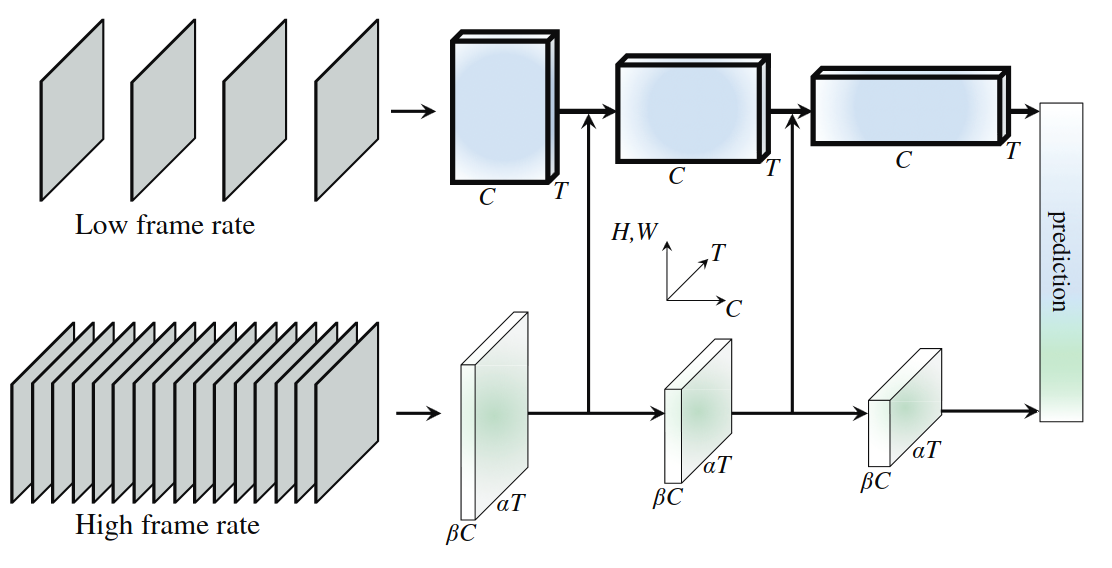
\includegraphics[width=0.5\textwidth]{imagenes/chapter2/SlowFastPathways.png}
  \end{center}
  \caption[Red convolucional espaciotemporal \emph{SlowFast}.]{Ejemplo extraído de~\cite{SlowFastNetworks} para ilustrar la distinción 
  entre la extracción espacial del camino ``\emph{slow path}'' (camino superior) y 
  de movimiento con el camino ``\emph{fast path}'' (camino inferior).}
  \label{fig:SlowFastPathways}
\end{figure}

\subsubsection{Aplicadas a nubes de puntos}

De forma similar al caso de lo vídeos, actualmente existen modelos de 3D CNN's 
capaces de procesar nubes de puntos al añadir una dimensión más que representa 
la profundidad de los puntos.  Sin embargo, la complejidad de diseño y tiempo de cómputo para 
estos modelos 3D crece enormemente. Ya que habitualmente las nubes de puntos 
están formadas por puntos dispersos en el espacio, en lo que denominamos datos 
sin estructura ni orden propio, y debemos mapear una operación 
de convolución que está basada en operaciones sobre datos ordenados y estructurados. 

Aunque cada vez hay más métodos que se aplican directamente sobre la nube de puntos 
desde la publicación de \emph{PointNet}~\cite{PointNet}, habitualmente se 
intenta estructurar la información de las nubes de puntos mediante lo que 
denominamos vóxeles~\cite{VoxelizationExample}. 
La voxelización es el proceso de transformar una nube de puntos u otra representación 
tridimensional en una estructura discreta conocida como volumen voxelizado. 
Esto implica dividir el espacio tridimensional en una cuadrícula de vóxeles y asignar 
valores a cada vóxel según la información contenida en los datos originales. 
La voxelización proporciona una representación estructurada y discreta que permite 
el uso de técnicas específicas para volúmenes y facilita el procesamiento y análisis 
de datos 3D.

\begin{figure}[htp]
  \centering
  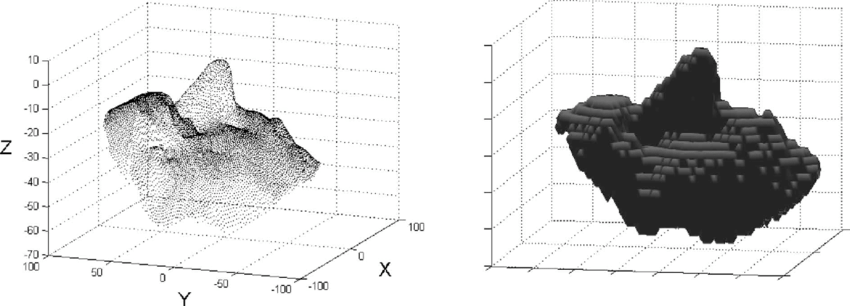
\includegraphics[width=0.80\textwidth]{imagenes/chapter2/VoxelizationExample.png}
  \caption[Ejemplo gráfico sobre voxelización.]{Ejemplo extraído de~\cite{VoxelizationExample} que demuestra el resultado 
  de transformar una nube de puntos sin estructura en una cuadrícula voxelizada.}
  \label{fig:VoxelizationExample}
\end{figure}

\subsection{Ensemble de modelos de Deep Learning}
Un \emph{ensemble}, en el contexto del aprendizaje automático, es una técnica que 
combina múltiples modelos de aprendizaje para mejorar la precisión y el rendimiento 
general de las predicciones. En lugar de depender de un único modelo, 
se crean múltiples modelos y se combinan sus predicciones para obtener un resultado 
final más robusto y preciso~\cite{IAModernApproach, DataMiningHandbook, MedicalEnsembleExample}.

La idea fundamental detrás de los \emph{ensembles} es que los diferentes modelos pueden 
tener fortalezas y debilidades diferentes, y al combinar sus predicciones, se 
puede obtener una mejor generalización y un mayor rendimiento en una variedad de 
situaciones. Para construir un \emph{ensemble} se suele utilizar un conjunto 
de técnicas que se describirán a continuación. 

El \emph{bagging} consiste en generar múltiples conjuntos de datos de entrenamiento 
mediante muestreo con reemplazo, entrenando un modelo en cada conjunto y 
promediando o ponderando sus predicciones. 
En el \emph{boosting}, los modelos se construyen secuencialmente, corrigiendo los errores 
del modelo anterior, y se combinan para formar un modelo más fuerte. 
La aumentación de datos consiste en ampliar el conjunto de entrenamiento para
mejorar la capacidad de generalización del modelo y reducir el sobreajuste por 
medio de transformaciones sobre los datos como la rotación y ampliación, 
se podría usar como paso en el proceso de \emph{bagging}.
Los \emph{random forests} combinan \emph{bagging} y árboles de decisión, 
generando múltiples árboles utilizando diferentes subconjuntos de datos y características. 
Las predicciones de los árboles individuales se combinan para obtener la predicción final.
Por último, el \emph{stacking} entrena múltiples modelos base y utiliza un meta-modelo 
para combinar sus predicciones. 
Cada estrategia tiene sus beneficios y consecuencias.

El presente TFG evalúa el uso de un meta-modelo para la estimación de calidad de 
las imágenes médicas 3D sin referencia.

\begin{figure}[htp]
  \centering
  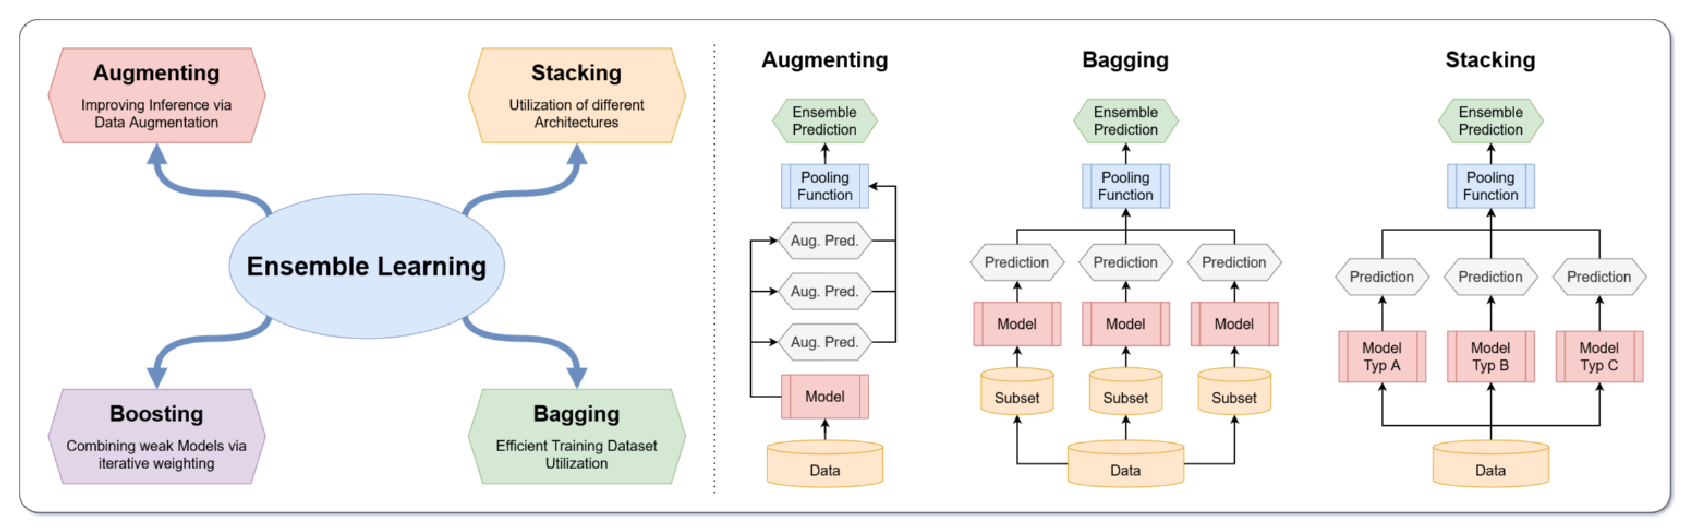
\includegraphics[width=\textwidth]{imagenes/chapter2/EnsembleExample.png}
  \caption[Representación de métodos de \emph{ensemble}.]{Representación de métodos de \emph{ensemble} extraído de~\cite{MedicalEnsembleExample}.}
  \label{fig:EnsembleExample}
\end{figure}

\section{Imágenes médicas y distorsiones}
\label{sec:Distorsiones}
Las tomografías computarizadas son un tipo de técnica de imagen médica 
que utiliza rayos X para obtener imágenes detalladas del interior del cuerpo. 
Durante una tomografía computarizada, el paciente se coloca en una mesa que se 
mueve a través de un anillo en forma de donut llamado \emph{gantry}. Dentro del \emph{gantry},
se encuentra un tubo de rayos X que gira alrededor del paciente, emitiendo haces 
de rayos X en forma de abanico.
Los detectores ubicados en el lado opuesto del \emph{gantry} registran la cantidad de 
rayos X que atraviesan el cuerpo del paciente. Estos datos se recopilan en 
múltiples ángulos y se utilizan para reconstruir imágenes transversales del cuerpo. 

\begin{figure}[htp]
  \begin{subfigure}{2\textwidth}
  \hspace{1cm}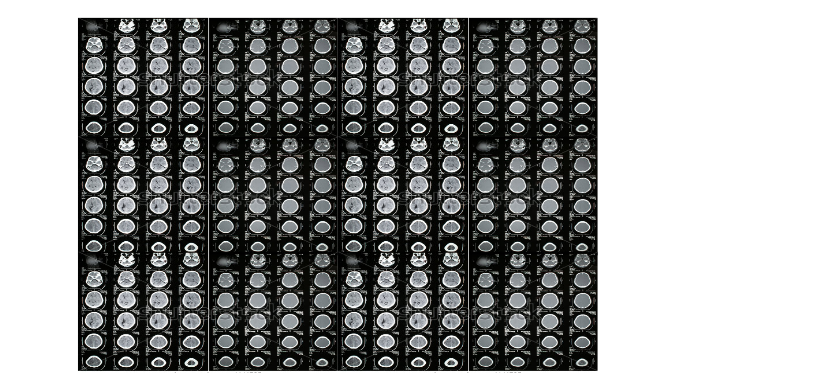
\includegraphics[width=0.5\textwidth]{imagenes/chapter2/CTDir.png}
  \end{subfigure}
  \begin{subfigure}{2\textwidth}
  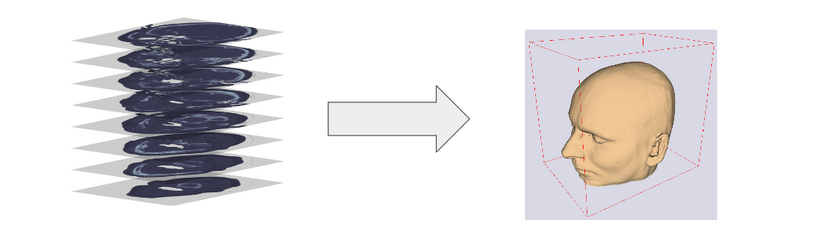
\includegraphics[width=0.5\textwidth]{imagenes/chapter2/CT2Volume.png}
  \end{subfigure}
  \caption[Ejemplo de tomografía computarizada y modelo 3D.]{Ejemplo de tomografía computarizada y modelo 3D~\cite{CT2Volume}.}
  \label{fig:CT2Volume}
\end{figure}

El número de imágenes en una tomografía computarizada se selecciona en función 
de varios factores, como el área del cuerpo que se está examinando, el propósito 
clínico de la exploración y las preferencias del radiólogo o médico que interpreta 
las imágenes. Ajustar el número de imágenes puede influir en el tiempo de adquisición, 
la cantidad de radiación utilizada y la cantidad de información detallada que se 
obtiene de la exploración. Afecta directamente a la calidad del modelo 3D generado 
al final ya que el número de cortes es la tercera dimensión que relaciona las imágenes 
(profundidad).

Sobre todo nos centraremos en las distorsiones geométricas que ocurren en la 
generación volumétrica de la imagen. La generación del volumen consiste en 
disponer de un conjunto segmentado\footnote{
La segmentación se refiere al proceso de dividir una imagen o conjunto de datos en regiones o componentes más pequeños. 
Ejemplo, en una foto del bosque, segmentamos los árboles para distinguirlos del suelo.
} en todas las capas de las imágenes. A continuación usando el conjunto segmentado 
unificamos las coordenadas de los puntos por medio de intersecciones entre rayos 
proyectados sobre las imágenes (\emph{ray casting}, véase Figura \ref{fig:CT2Volume}).

% \begin{figure}[htp]
%   \centering 
%   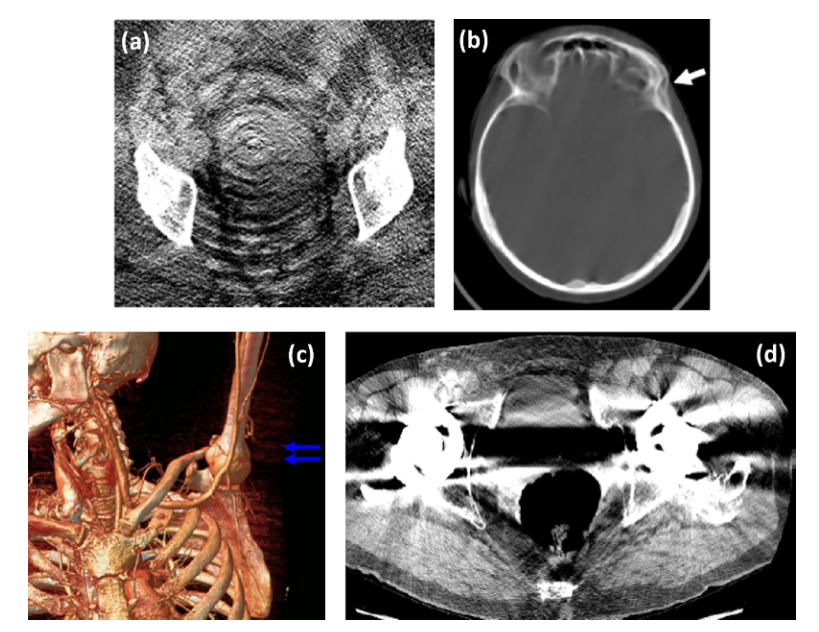
\includegraphics[width=\textwidth]{imagenes/chapter2/DicomDistortionsExample.png}
%   \caption[Ejemplo de artefactos sobre imágenes DICOM.]{Ejemplo de artefactos sobre imágenes DICOM~\cite{DicomDistortionsExample}: 
%   (a) un artefacto de anillo, (b) un difuminado provocado por movimiento, 
%   (c) artefactos producidos por interpolación helicoidal, (d) artefactos de iluminación y dispersión del haz.  }
%   \label{fig:DicomDistortionsExample}
% \end{figure}

Dentro de las causas de las distorsiones geométricas sobre los volúmenes 
3D están el difuminado por movimiento, errores de contraste (dificultad al segmentar),
artefactos luminosos y problemas de interpolación o ruido al generar la proyección (véase Figura \ref{fig:DicomDistortionsExample}). 

Para simularlo, partiremos de ejemplos de imágenes médicas consideradas exentas de 
distorsiones, con su segmentación correspondiente realizada por profesionales.
A continuación, generaremos la representación volumétrica como una nube de puntos 
y sobre ella simularemos las distorsiones. 

Dos de ellas serán para simular los resultados de varios algoritmos de compresión, 
como puede ser \emph{octree compression}~\cite{OctreeCompression} y la reducción de número de puntos 
por medio de submuestreo aleatorio (en inglés \emph{random downsampling}). 
Un \emph{octree} es una representación más eficiente que los vóxeles, se trata 
de la descomposición de forma recursiva de la escena en 8 partes hasta 
la profundidad máxima, donde cada nodo representa un cubo tridimensional 
llamado octante. En la compresión se analiza los octantes y se elimina los que aportan 
menos información. 
En el segundo, establecemos un porcentaje de puntos que eliminar y los eliminamos 
de forma aleatoria hasta alcanzar ese porcentaje de reducción.

Las demás representarán efectos que podrían ocurrir por desplazamiento de los puntos, 
como el movimiento del paciente y aquellos provocados por ruido en la transmisión de datos.

\begin{figure}[htp]
  \begin{subfigure}[b]{.5\textwidth}
    \centering
    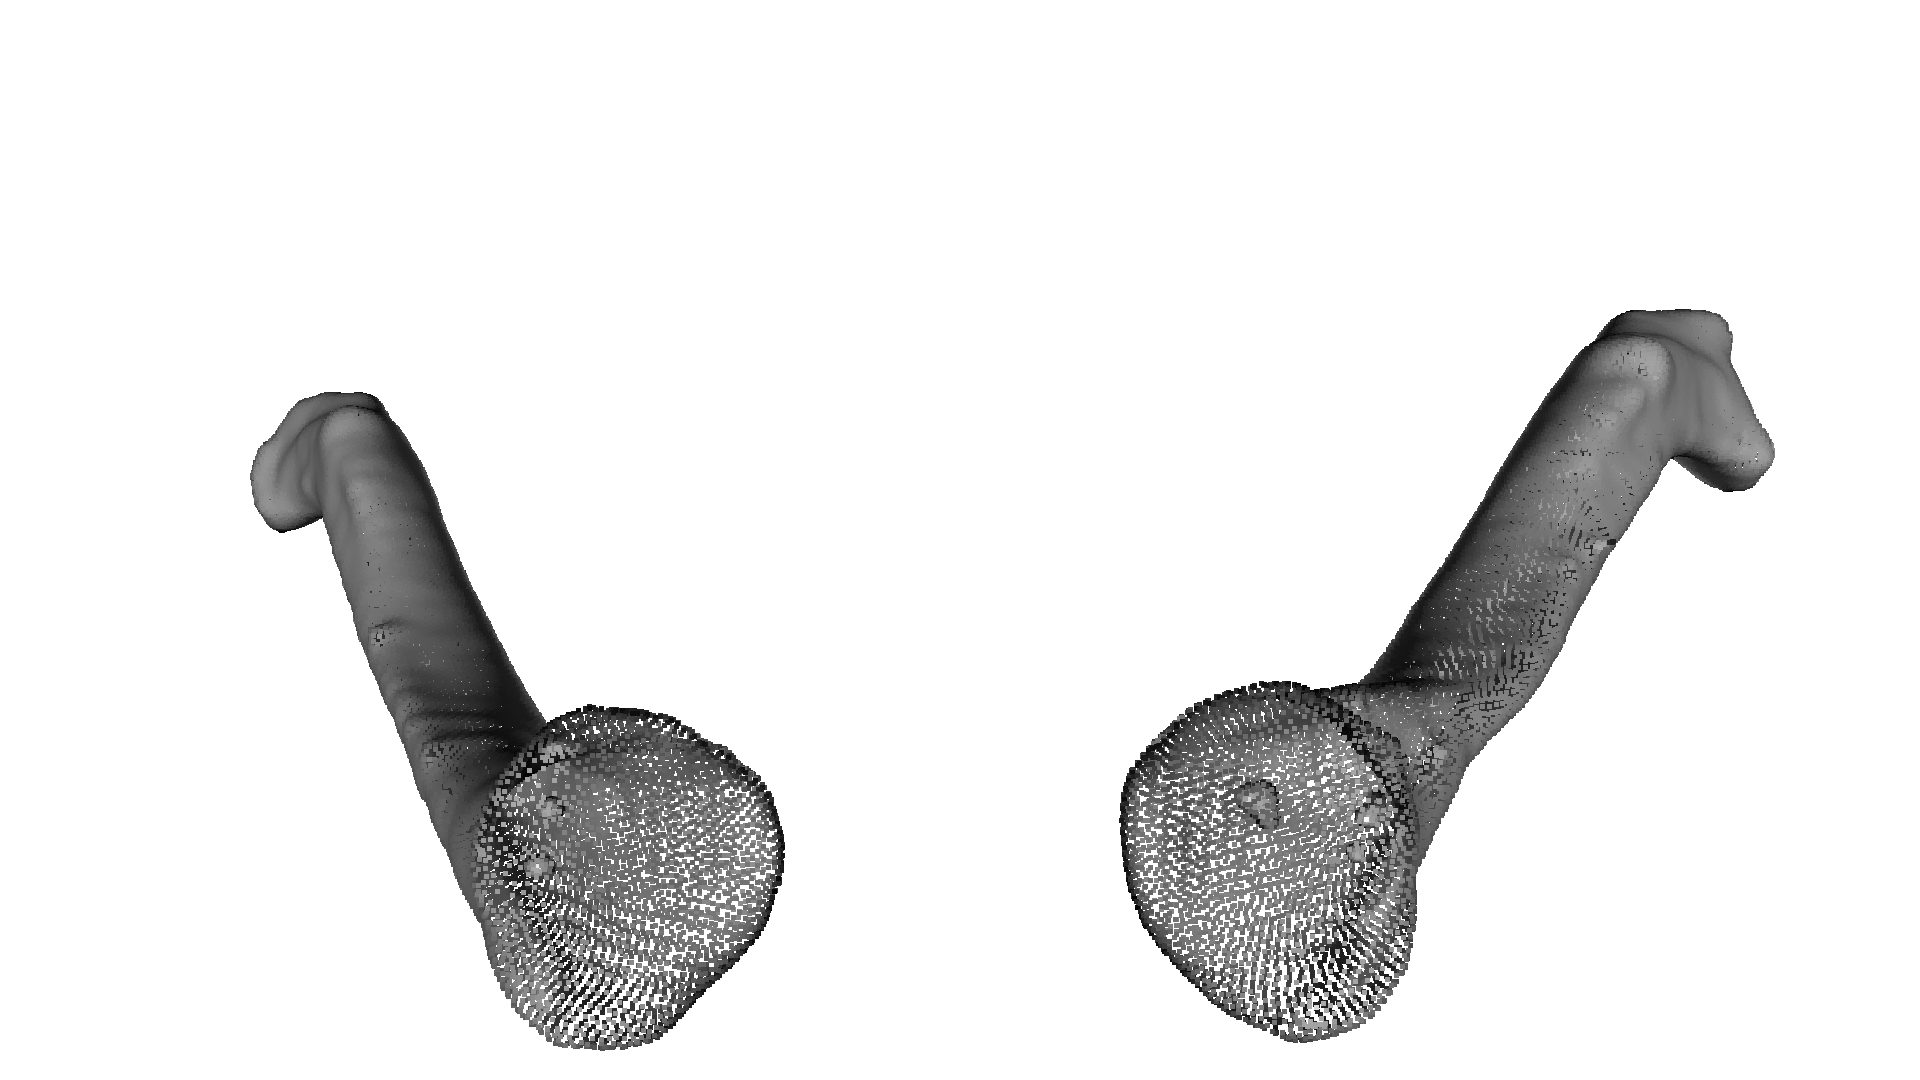
\includegraphics[width=\textwidth]{imagenes/chapter2/clavicula/clavicula_0.png}
  \end{subfigure}
  \hfill
  \begin{subfigure}[b]{.5\textwidth}
    \centering
    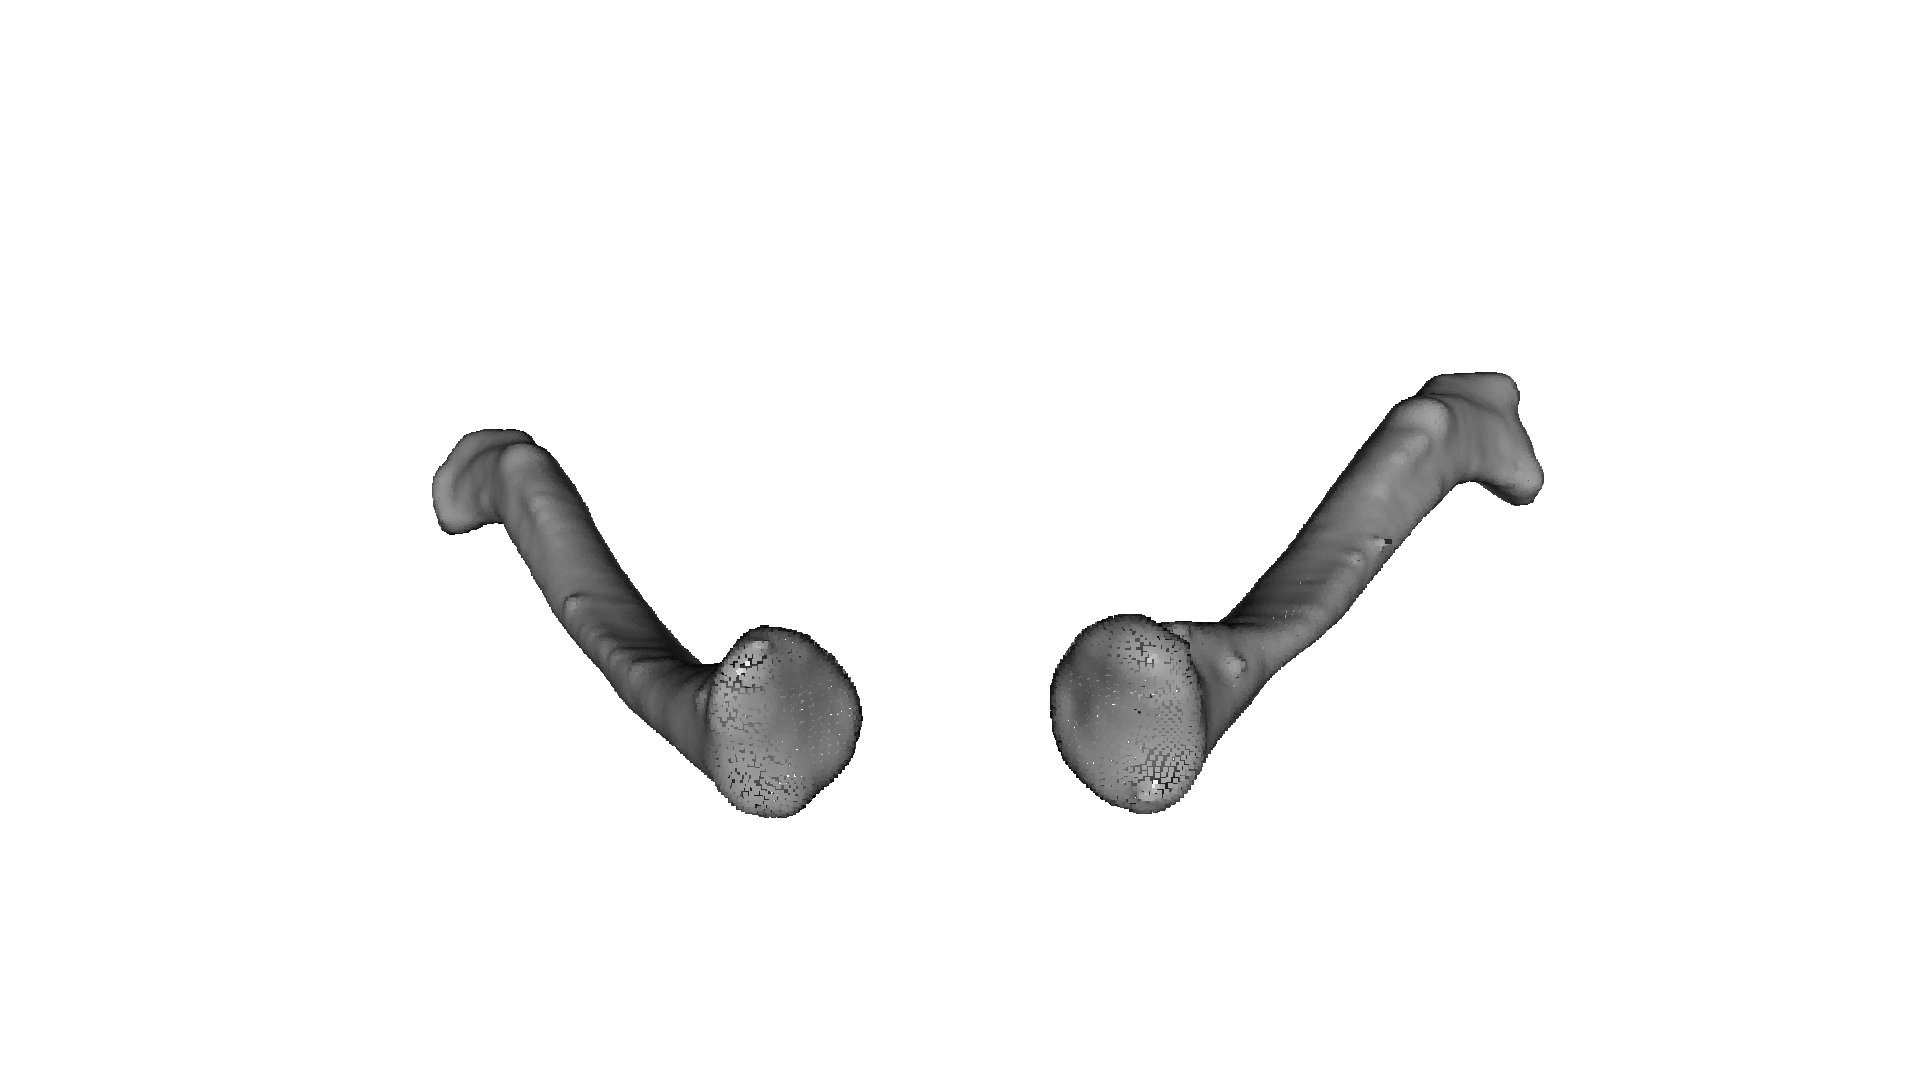
\includegraphics[width=\textwidth]{imagenes/chapter2/clavicula/clavicula_1.png}
  \end{subfigure}
  \begin{subfigure}[b]{.5\textwidth}
    \centering
    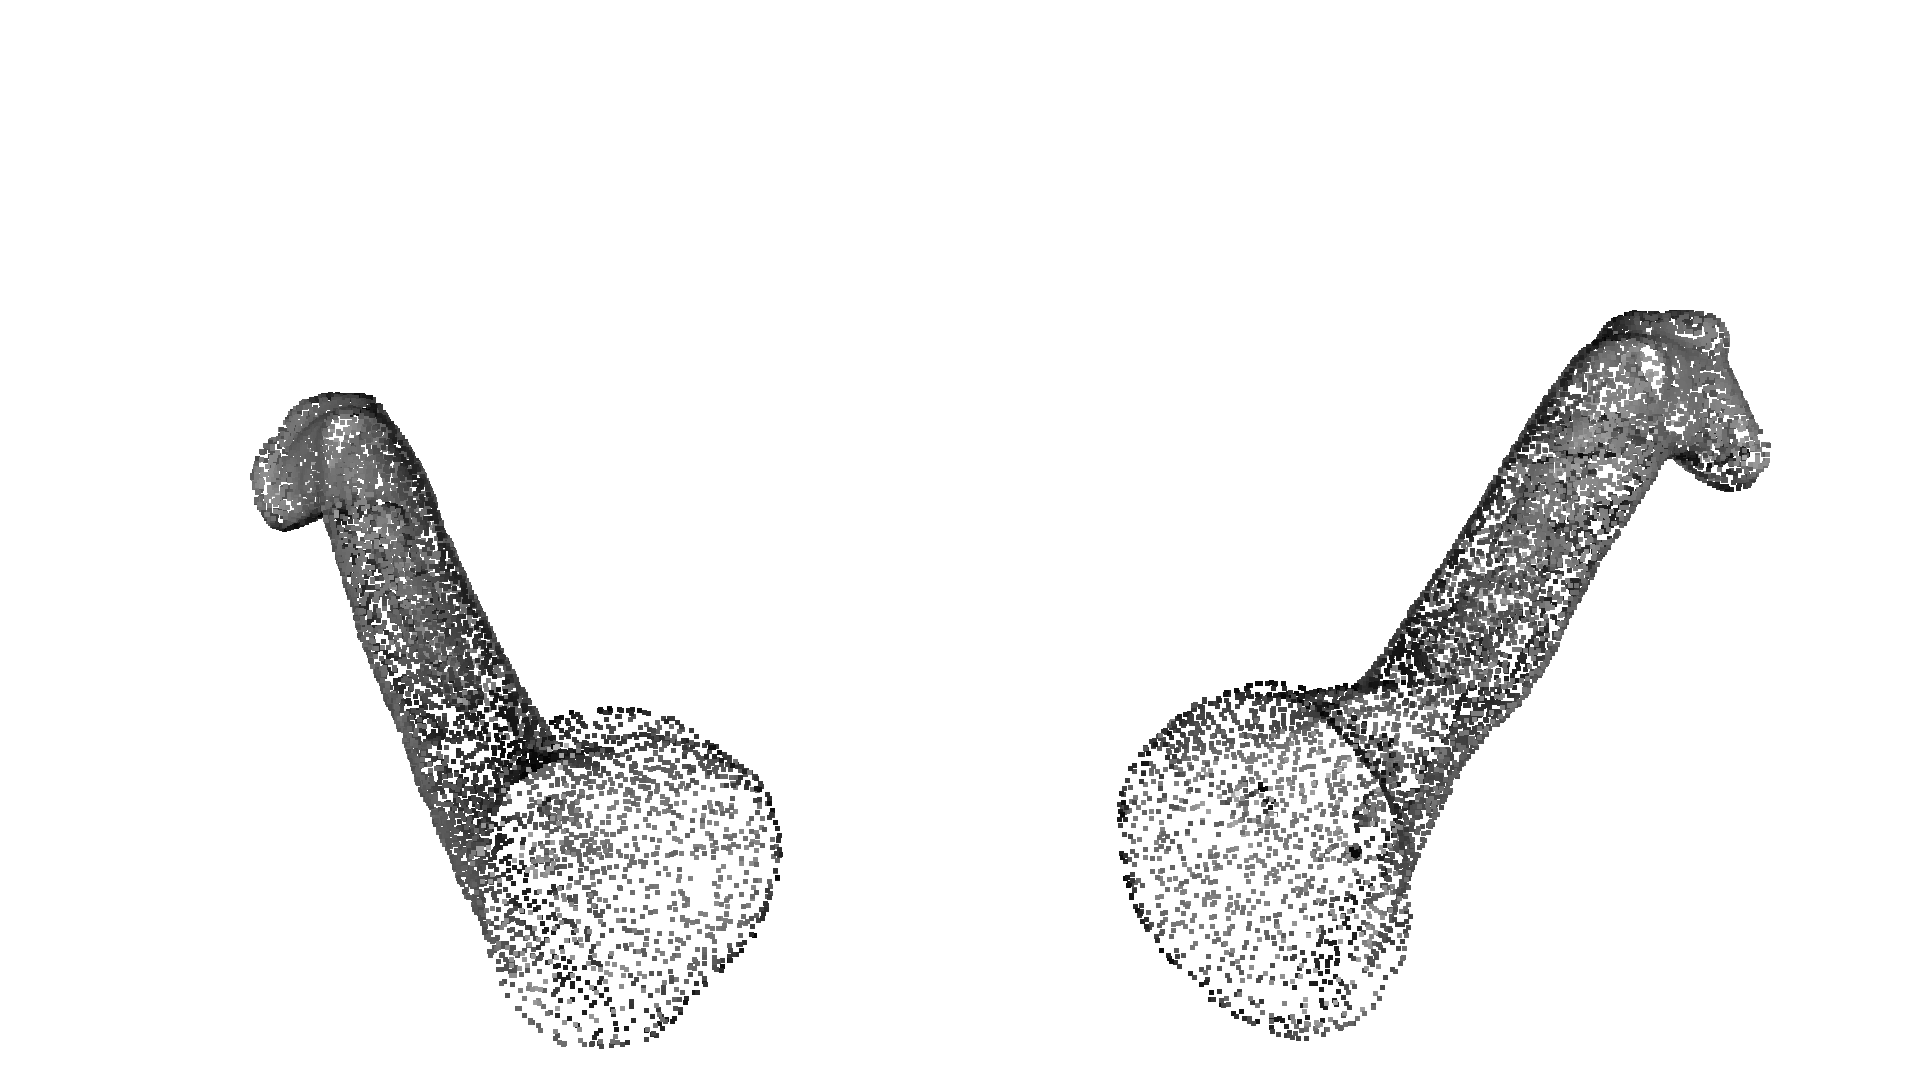
\includegraphics[width=\textwidth]{imagenes/chapter2/clavicula/clavicula_2.png}
  \end{subfigure}
  \hfill
  \begin{subfigure}[b]{.5\textwidth}
    \centering
    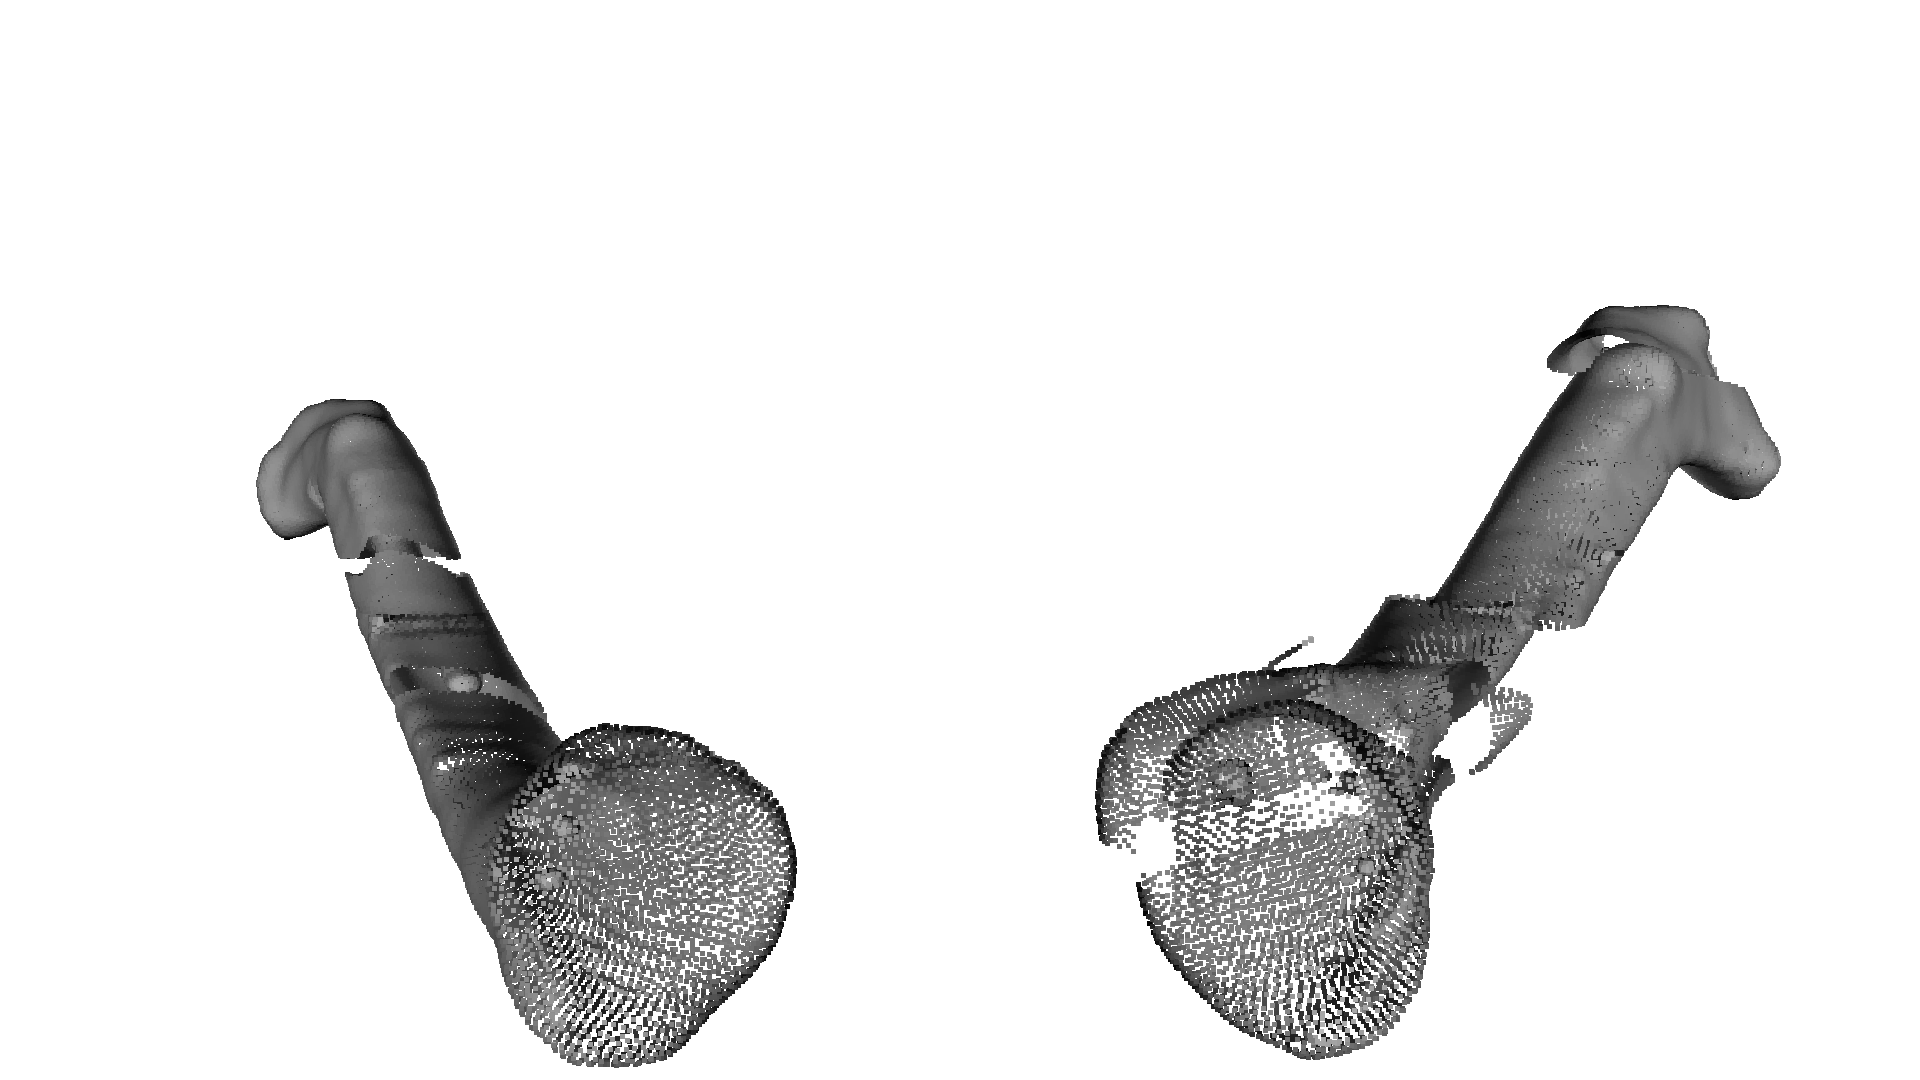
\includegraphics[width=\textwidth]{imagenes/chapter2/clavicula/clavicula_3.png}
  \end{subfigure}
  \begin{subfigure}[b]{.5\textwidth}
    \centering
    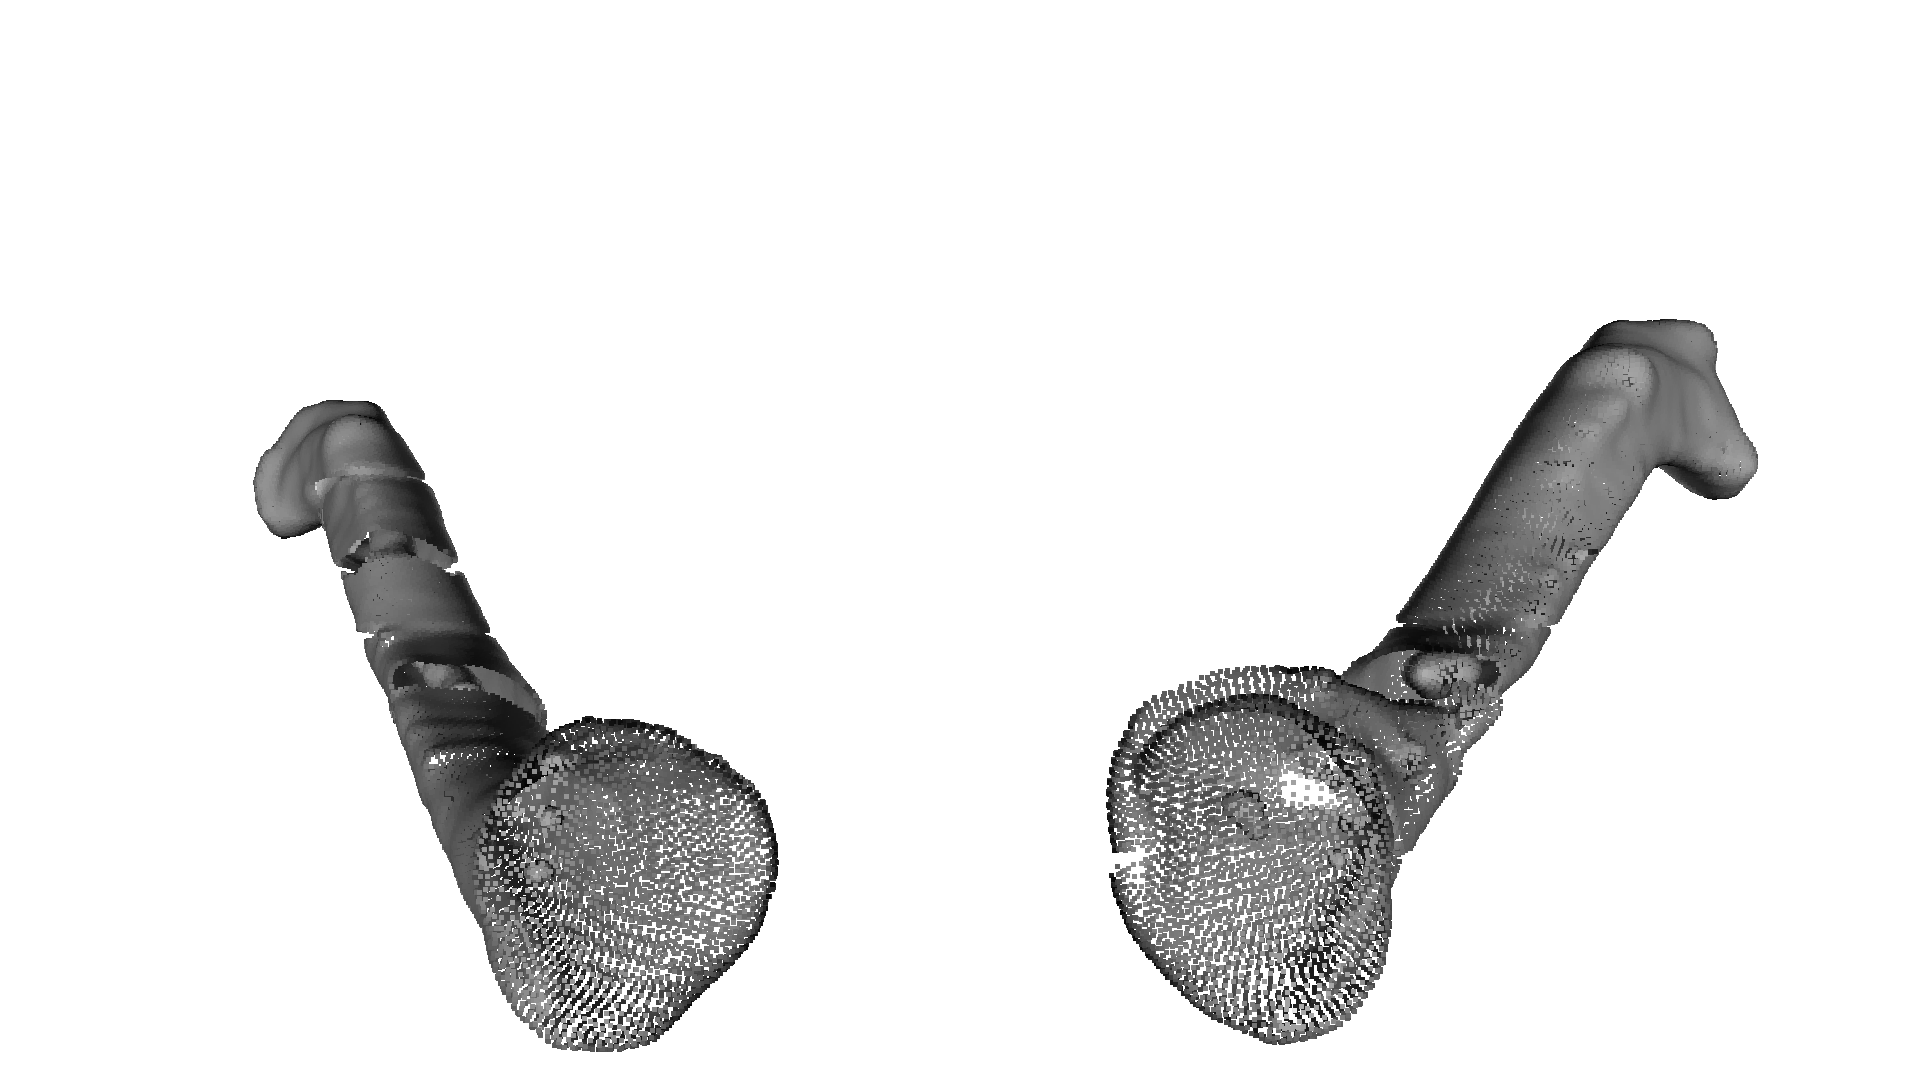
\includegraphics[width=\textwidth]{imagenes/chapter2/clavicula/clavicula_4.png}
  \end{subfigure}
  \begin{subfigure}[b]{.5\textwidth}
    \centering
    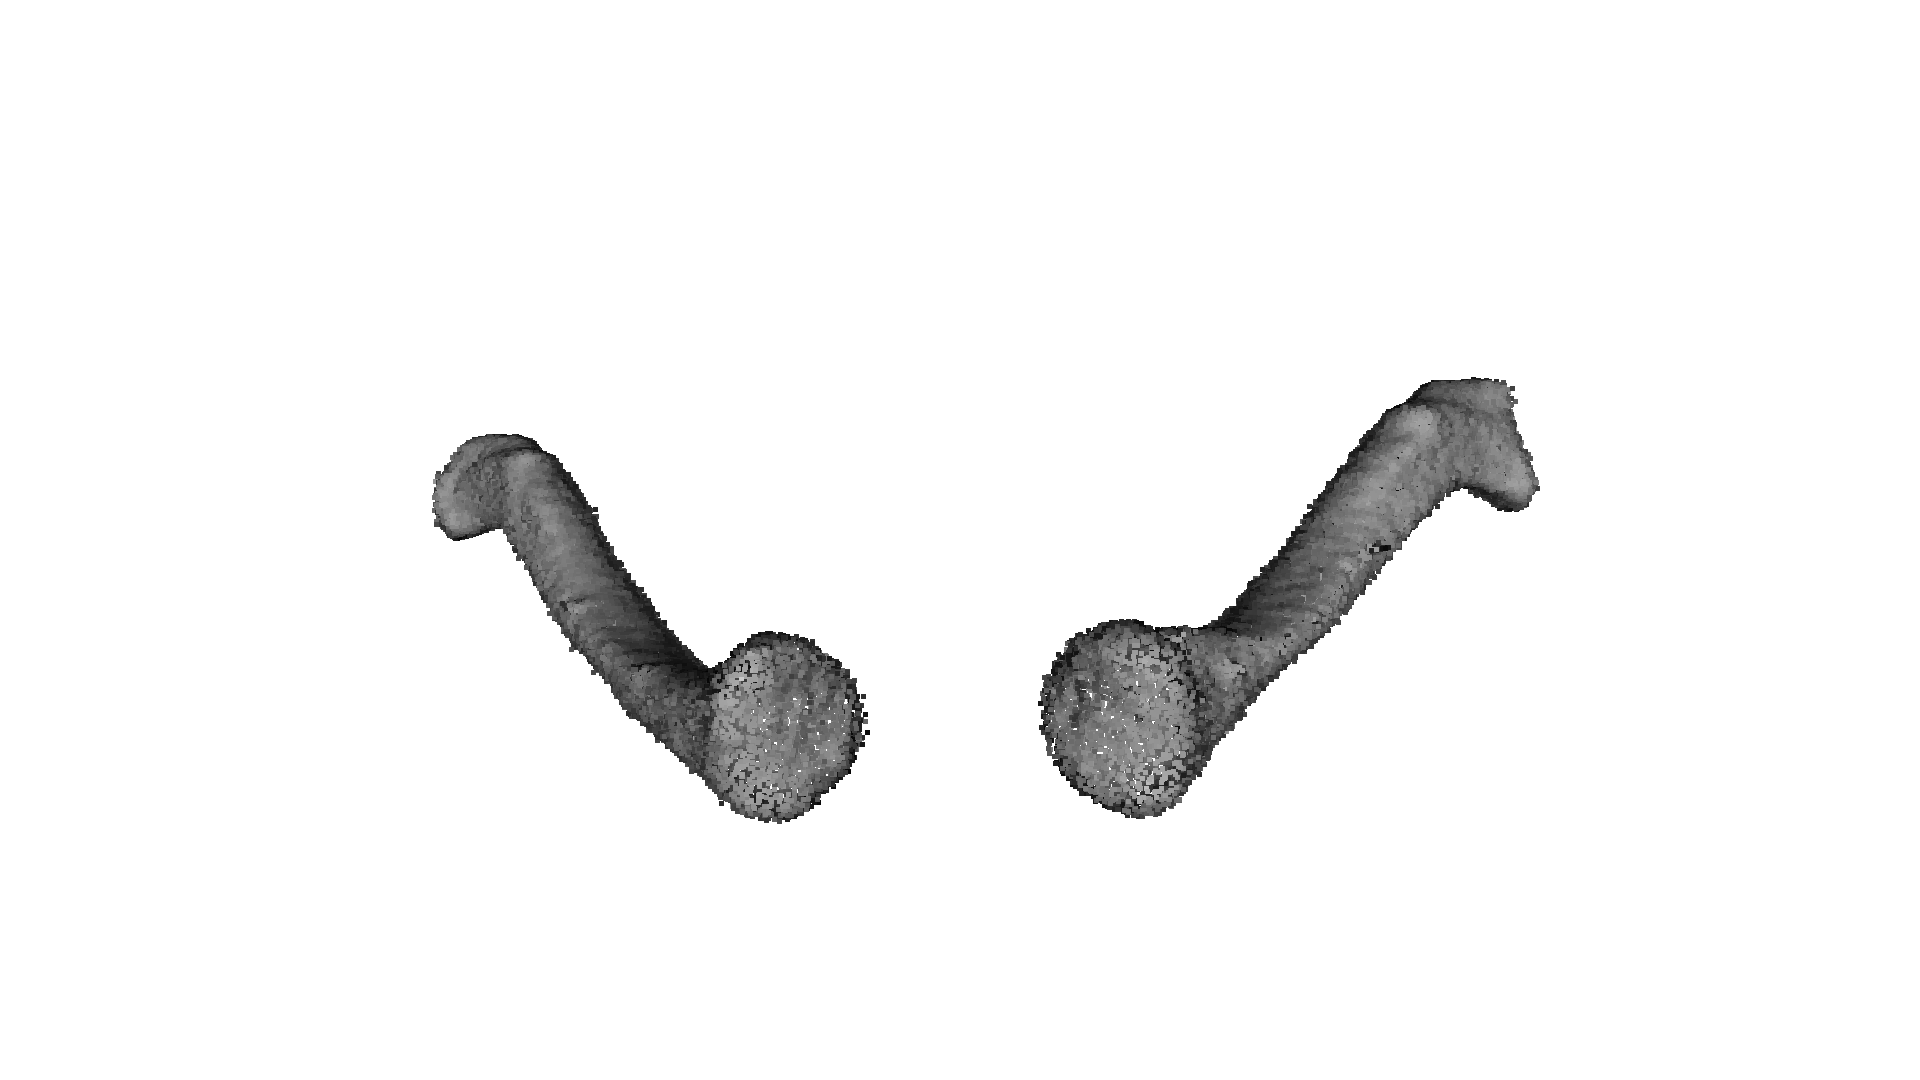
\includegraphics[width=\textwidth]{imagenes/chapter2/clavicula/clavicula_5.png}
  \end{subfigure}
  \caption[Ejemplo de distorsiones generadas sobre clavículas.]{Ejemplo de distorsiones generadas sobre clavículas. Leyendo de izquierda a derecha tenemos:
    la imagen original, compresión \emph{octree}, reducción de puntos por \emph{random downsampling},
    movimiento local, rotación local y ruido gaussiano.
  }
  \label{fig:DistorsionesGeneradas}
\end{figure}

% %
\chapter{Estado del Arte}
\label{sec:EstadoDelArte}

\begin{figure}[htp]
  \centering
  \begin{subfigure}{0.47\textwidth}
    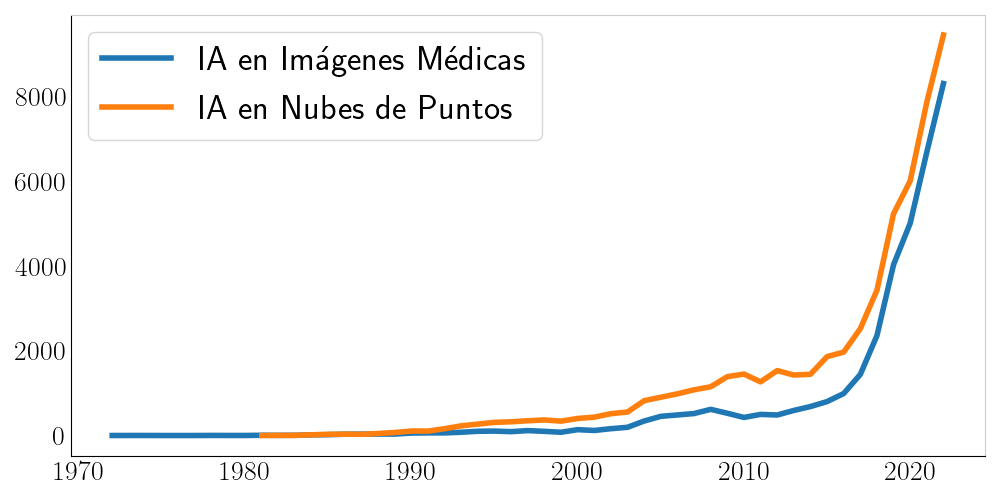
\includegraphics[width=\textwidth]{imagenes/chapter3/ScopusMLinMedicineAndPC.png}
  \end{subfigure}
  \begin{subfigure}{0.47\textwidth}
    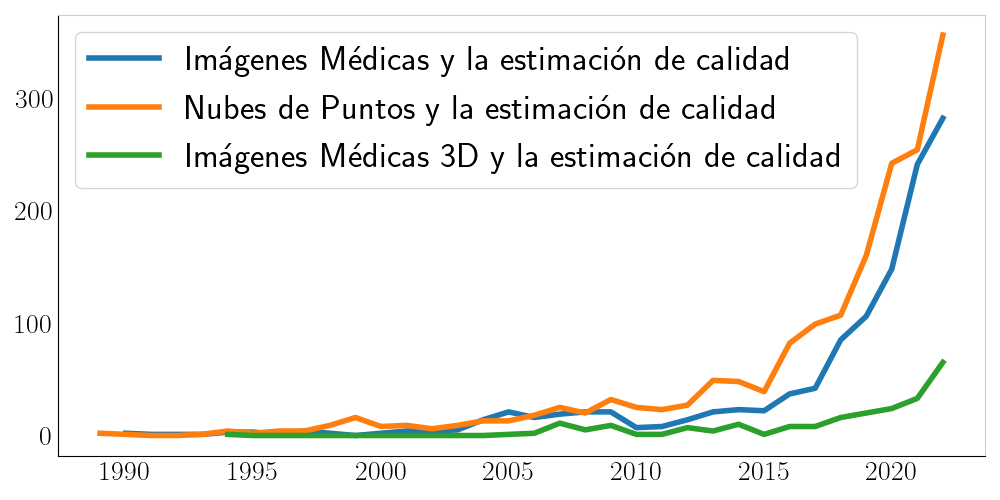
\includegraphics[width=\textwidth]{imagenes/chapter3/ScopusQualityAssessment.png}
  \end{subfigure}
  \caption{Ejemplo de crecimiento de interes en el campo según \emph{Scopus}\footnotemark[1].
  }
  \label{fig:ScopusMLinMedicalAndPC}
\end{figure}
\footnotetext[1]{
Las búsquedas se pueden consultar en el apéndice.
}


\towrite[{Escribir búsquedas en Corpues}]{Hacer introducción y historial de búsqueda de artículos}

Las métricas más populares para la estimación objetiva de la calidad de modelos 
3D basada en puntos son \emph{point-to-point} (Po2Po)\cite{PointToPoint} y
\emph{point-to-plane} (Po2Pl)\cite{PointToPlane}. 
En la primera, para cada punto del objeto distorsionado se obtiene su vecino más cercano en la versión de referencia y 
se calcula alguna métrica de distancia como las discutidas anteriormente (MSE, Minkowski, Hausdorff...). 
La principal desventaja de estos modelos es que no consideran los objetos como 
superficies, aparte de lo comentado en (\ref{fig:FailureMinkowskiMetric},\ref{fig:MSEHyperSphere}).
Para solventar este problema se formuló el segundo método por Tian \emph{et al.} 
que modela la superficie en cada punto como un plano. Ese plano es perpendicular a 
la normal en cada punto. Que se calcula en base a la información de su vencindario. Es decir, 
realizamos los mismos pasos que para la primera, pero proyectamos la distancia sobre 
el vector normal correspondiente. 

Se propuso también otra métrica como \emph{Plane-to-Plane} (Pl2Pl)\cite{PlaneToPlane}, 
que mide la similitud entre superficies associadas a las nubes de puntos. Dentro 
de este mismo ámbito surge también \emph{Point-to-Surface}\cite{PlaneToSurface}, 
que mide la distancia de cada punto de la versión distorsionado respecto a su 
superficie correspondiente en la nube de referencia. Luego para poder tener en
cuenta los colores, surgieron métricas como Po2Po PSNR\cite{PSNR} donde la diferencia 
ya no es respecto a la posición del punto sino que al color en el espacio $YC_bC_r$.

De la información del vecindario de los puntos, gran cantidad de información geométrica 
puede ser extraída para investigar en profundidad la similitud entre las nubes 
de puntos. Surgieron métodos basados en la extracción de características donde la 
mayoría considera tanto información geométrica como los atributos lumínicos.
Existe apenas una métrica que apenas considera características geométricas: PC-MSDM \cite{PC-MSDM}. 
Es una métrica que busca la similitud estructural entre nubes de puntos basándose en
las estadísticas locales de curvatura de los puntos. Esta junto a la información 
extraída de los colores dió lugar a una métrica de similitud de estructuras\cite{PointSSIM}
como adaptación del método \cite{StructuralSimilarityIndex} de IQA a nubes de puntos\cite{SSIM}.  Experimentando con combinaciones de 3 medidas geométricas y 5 comparaciones de color 
para encontrar el mejor vector características resultó en la metrica PCQM\cite{PCQM}.
Similar, utilizando el análisis de componentes principales (PCA) en un vecindario 
de puntos para extraer los valores y vectores singulares por cada punto permitió 
obtener buenos descriptores de información geométrica\cite{PointPCA}.

También se estudió las componentes lumínicas de las nubes de puntos en \cite{ColorBasedObjectiveMetricPC, BitDance}. 
Consistía en generar un histograma y correlograma de la componente lumínica. 
Un correlograma nos permite caracterizar la relación entre pares de variables 
numéricas en un conjunto de datos. Otros, velaron por estudio la energia potencial 
en las nubes de puntos y las diferencias que emergen en presencia de distorsiones\cite{PotentialEnergy}.
Incluso se investigó las transformaciones de datos, se construyeron grafos que representan 
las nubes de puntos, tanto la de referencia como la distorsionada, 
para producir métricas de similitud como GraphSIM y MS-GraphSim\cite{GraphSIM, MS-GraphSim}.

De igual forma, se adaptaron ideas de otros ámbitos, por ejemplo, utilizando 
proyecciones que transladan el mundo tridimensional a un espacio 2D para utilizar 
los métodos más conocidos de estimación de calidad en 2D.
Se realizó incluso un estudio sobre el impacto del número de proyecciones 2D de 
distintas perspectivas en el rendimiento de las métricas de calidad \cite{ImpactOf2DProyections}.

Sin embargo, cuando no tenemos acceso a la nube de puntos de referencia, todas 
estas métricas se ven inutilizables. \emph{Viola et at.}\cite{ViolaRR} propuso 
transferir ciertas características de la nube de punto original antes del proceso
de compresión y transmisión. Con esa información adicional la nube de puntos 
resultantes puede ser evaluada sin la nube de referencia.

\towrite[{Enlazar métodos FR/RR con su casi-similitud a NR}]{Describir similitud en el paso de extracción de características y otros métodos SOTA NR}

% %
\chapter{Materiales y Métodos}
\section{Materiales}
\subsection{Datos públicos} 
\label{sec:DatosPublicos}
Para este TFG se han utilizado diversos conjuntos de datos públicos para la 
evaluación y elección de los modelos anteriormente descritos. De entre ellos 
están SJTU\cite{SJTU}, WPC\cite{WPC1,WPC2} y LS-SJTU-PCQA\cite{ResSCNN} que tratan 
de conjuntos de nubes de puntos generalistas, de personas, animales y objetos cotidianos.

El primero de ellos parte de 10 nubes de puntos de referencia, ver Figura \ref{fig:SJTU}, 
a las cuales se aplican 7 tipos de distorsiones. Estas son: compresión, ruido 
al color, ruido geométrico, ruido gaussiano y combinación entre ellas, ver Tabla \ref{tab:SJTU}. Todas se aplican en una escala creciente
de intensidad del 1 al 6. Luego, se obtiene un MOS de 10 individuos para las 420 
nubes de puntos que sirve como medida de calidad de las mismas y para evaluar las predicciones del modelo.

\begin{figure}[htp]
  \centering 
    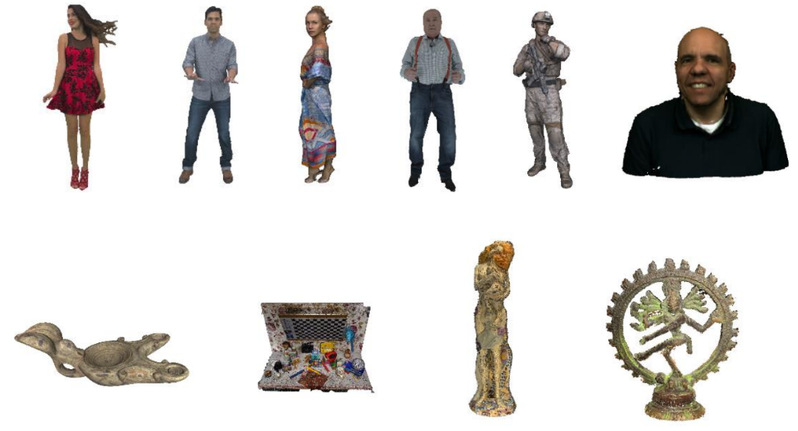
\includegraphics[width=0.75\textwidth]{imagenes/chapter4/SJTU}
    \caption{Ejemplo de conjuntos de datos SJTU\cite{SJTU}.}
    \label{fig:SJTU}
\end{figure}

\begin{table}[htp]
  \centering 
  \scriptsize
  \begin{tabular}{|c|c|}
    \hline
    \rowcolor[HTML]{FFC702}
    \textbf{Número} & \textbf{Tipo de Distorsión} \\ 
    \hline 
    0 & OT: Compresión octree\cite{OctreeCompression} \\ 
    \hline 
    1 & CN: Ruido fotométrico\\ 
    \hline 
    2 & DS: Submuestreo uniforme \\
    \hline 
    3 & DS + CN \\
    \hline 
    4 & DS + GGN \\
    \hline 
    5 & GGN: Ruido geométrico gaussiano \\
    \hline 
    6 & CN + GGN \\ 
    \hline 
  \end{tabular}
  \caption{Ejemplo de distorsiones en SJTU\cite{SJTU}.}
  \label{tab:SJTU}
\end{table}

El segundo dataset, WPC\cite{WPC1, WPC2}, también posee distorsiones como submuestreo uniforme y 
ruido gaussiano (aplicados de manera distinta), pero a su vez posee nuevos tipos 
de distorsiones. Estos son basados en distintos tipos de compresión: V-PCC, G-PCC y \emph{trisoup}.
Además, posee distintos tipos de nubes de puntos, ver Figura \ref{fig:WPC}, que 
pueden influir en el rendimiento del modelo si el conjunto no es
suficientemente amplio y representativo de lo que puede encontrarse una vez entrenado. 

\begin{figure}[htp]
  \begin{center}
    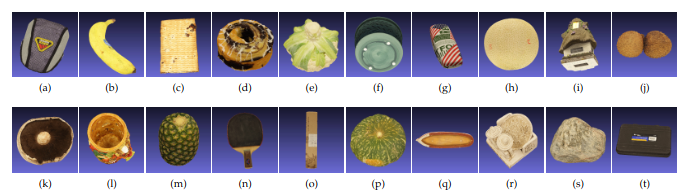
\includegraphics[width=0.95\textwidth]{imagenes/chapter4/WPC}
  \end{center}
  \caption{Ejemplo de conjunto de datos WPC\cite{WPC1, WPC2}.}
  \label{fig:WPC}
\end{figure}

Los dos anteriores han sido utilizados sobre todo para la evaluación y elección 
del modelo de regresión a utilizar. Son los conjuntos de datos más conocidos 
y que habitualmente están presentes en las publicaciones más recientes. Además, se realizaron 
pruebas de ejecuciones de algunos métodos de código abierto para verificar los 
resultados. Sin embargo, es el último es el que finalmente se utiliza para entrenar un modelo para estimar 
la calidad de las imágenes médicas. Esto es porque LS-SJTU-PCQA\cite{ResSCNN} 
es el mayor conjunto de datos 
en el momento de escritura, y posee tipos de distorsiones que pueden simular 
lo que sería ciertos errores y ruidos presentes en imágenes médicas. Por ejemplo, 
el ruido gaussiano (simular errores de transmisión y almacenado de datos), 
rotación y movimiento local (simular el movimiento del paciente) y compresión 
octree y por submuestreo uniforme (algoritmos de compresión comúnmente usados).
Aparte, es el con mayor amplitud de modelos base, con distintos tipos y categorías 
de objetos. Ver Figura \ref{fig:LS-SJTU-PCQA}.

\begin{figure}[htp]
  \begin{center}
    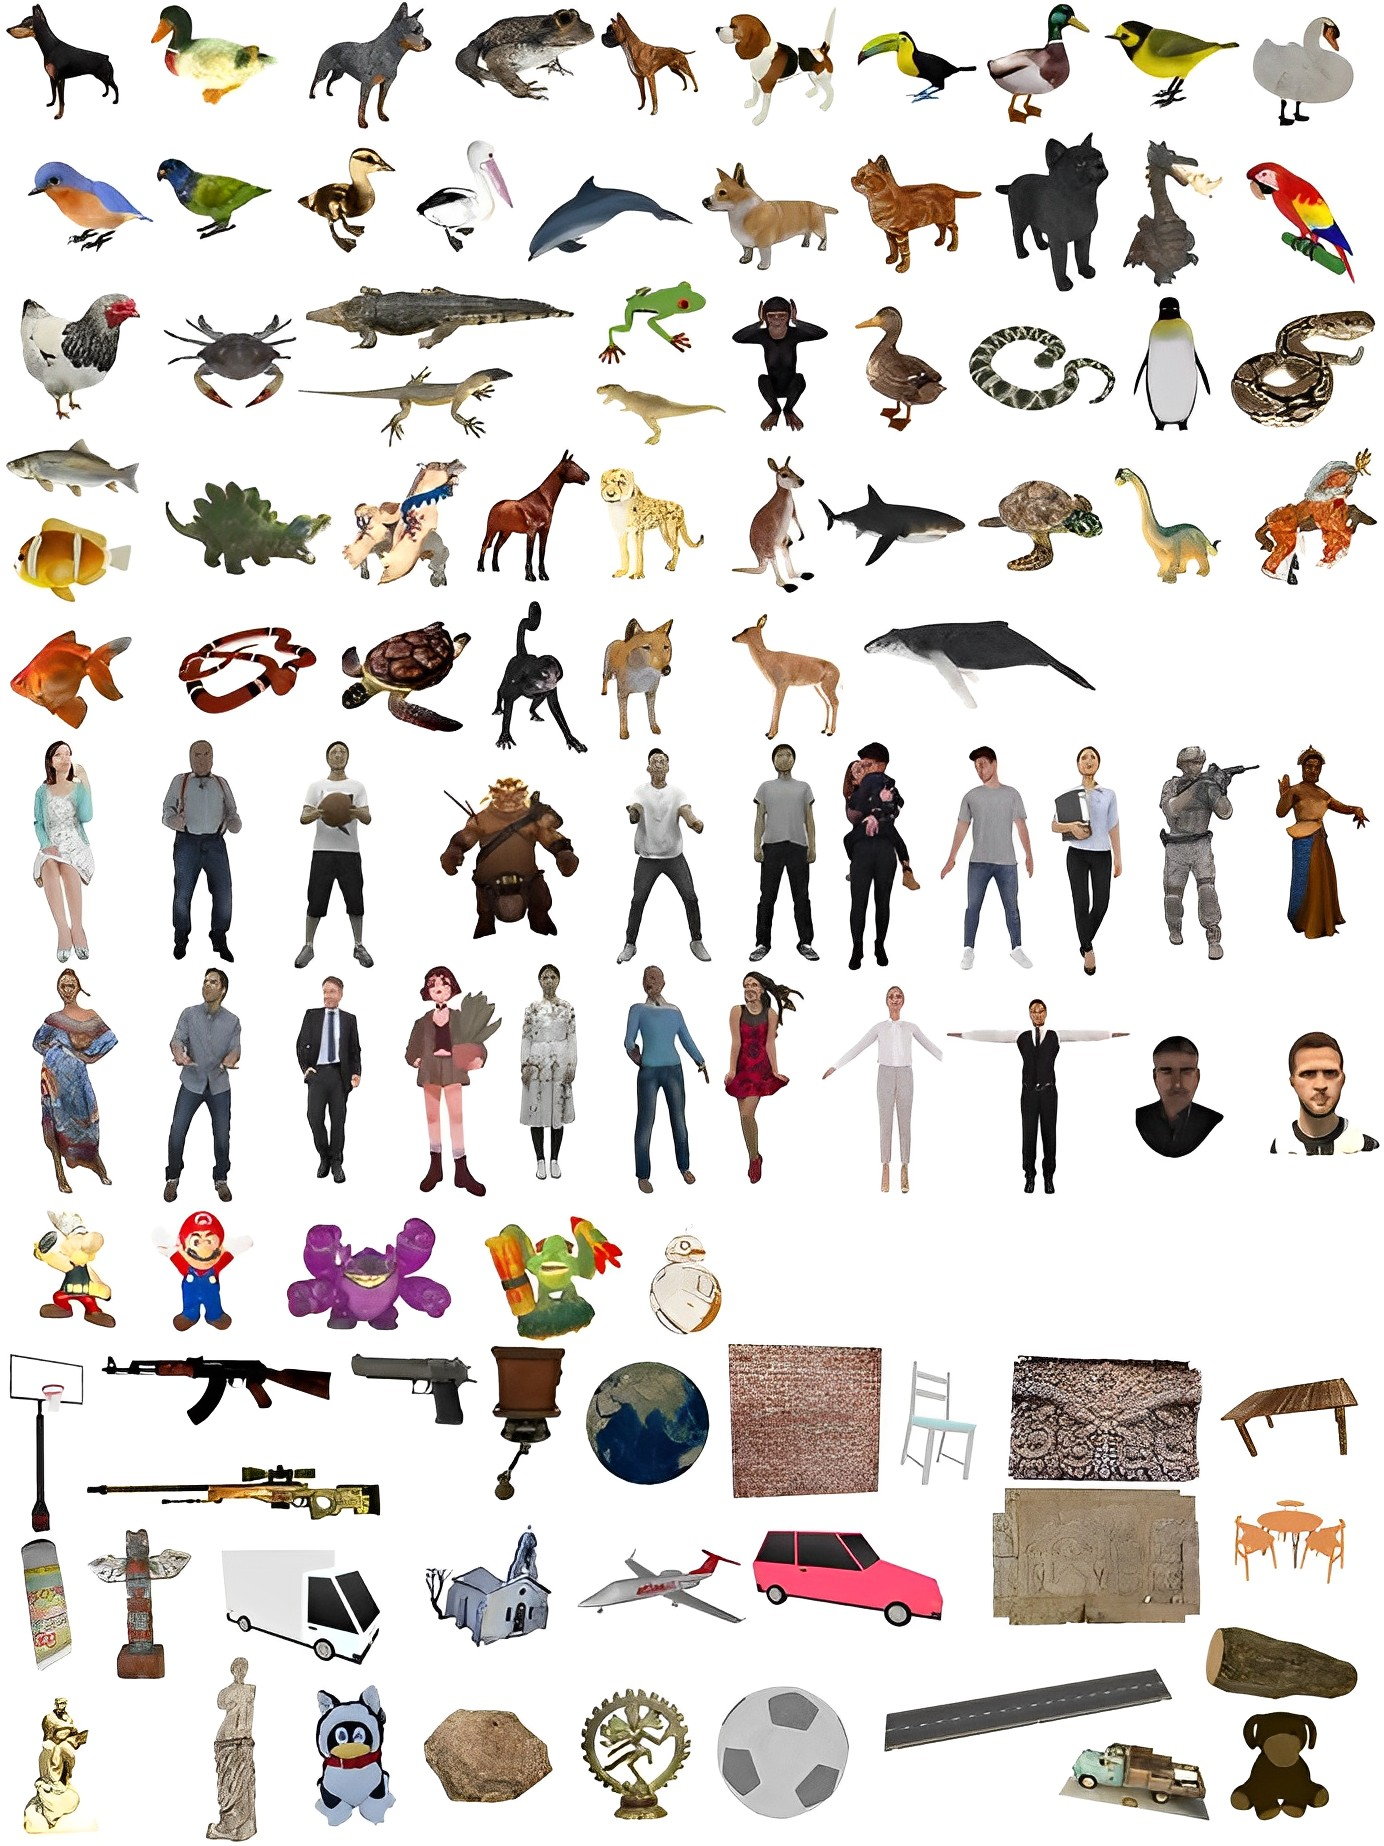
\includegraphics[width=0.95\textwidth]{imagenes/chapter4/LSPCQA}
  \end{center}
  \caption{Ejemplo de conjunto de datos LS-SJTU-PCQA\cite{ResSCNN}.}
  \label{fig:LS-SJTU-PCQA}
\end{figure}

\subsection{Conjunto de datos médicos}
\label{sec:OurData}
Para este TFG se tiene disponible una colección tomografías computerizadas, de distintas
partes del cuerpo, de 2 individuos distintos. 
De los cuales han sido segmentados las clavículas, el seno frontal y los senos maxilares. 
A parte, disponemos de volúmenes del cráneo de otros 3 individuos, una pubis izquierda y
una pubis derecha, ver Figura \ref{fig:OurDataExample}. Es decir, en total disponemos de 11 nubes de puntos de alta 
calidad, que representan distintos volúmenes de exámenes médicos.
A estos datos no se hicieron ningún tipo de pre-procesado, apenas se centraron 
las nubes de puntos a los ejes (operación necesaria para hacer la rotación para 
las distintas perspectivas, más detalles en la sección \ref{sec:Implementacion})
y se eliminaron aquellos puntos aislado de todos, frutos de errores en el 
algoritmo de reconstrucción 3D de las nubes de puntos a partir de segmentaciones DICOM.

\begin{figure}[htp]
  \centering
  \begin{subfigure}[b]{0.40\textwidth}
  \centering 
  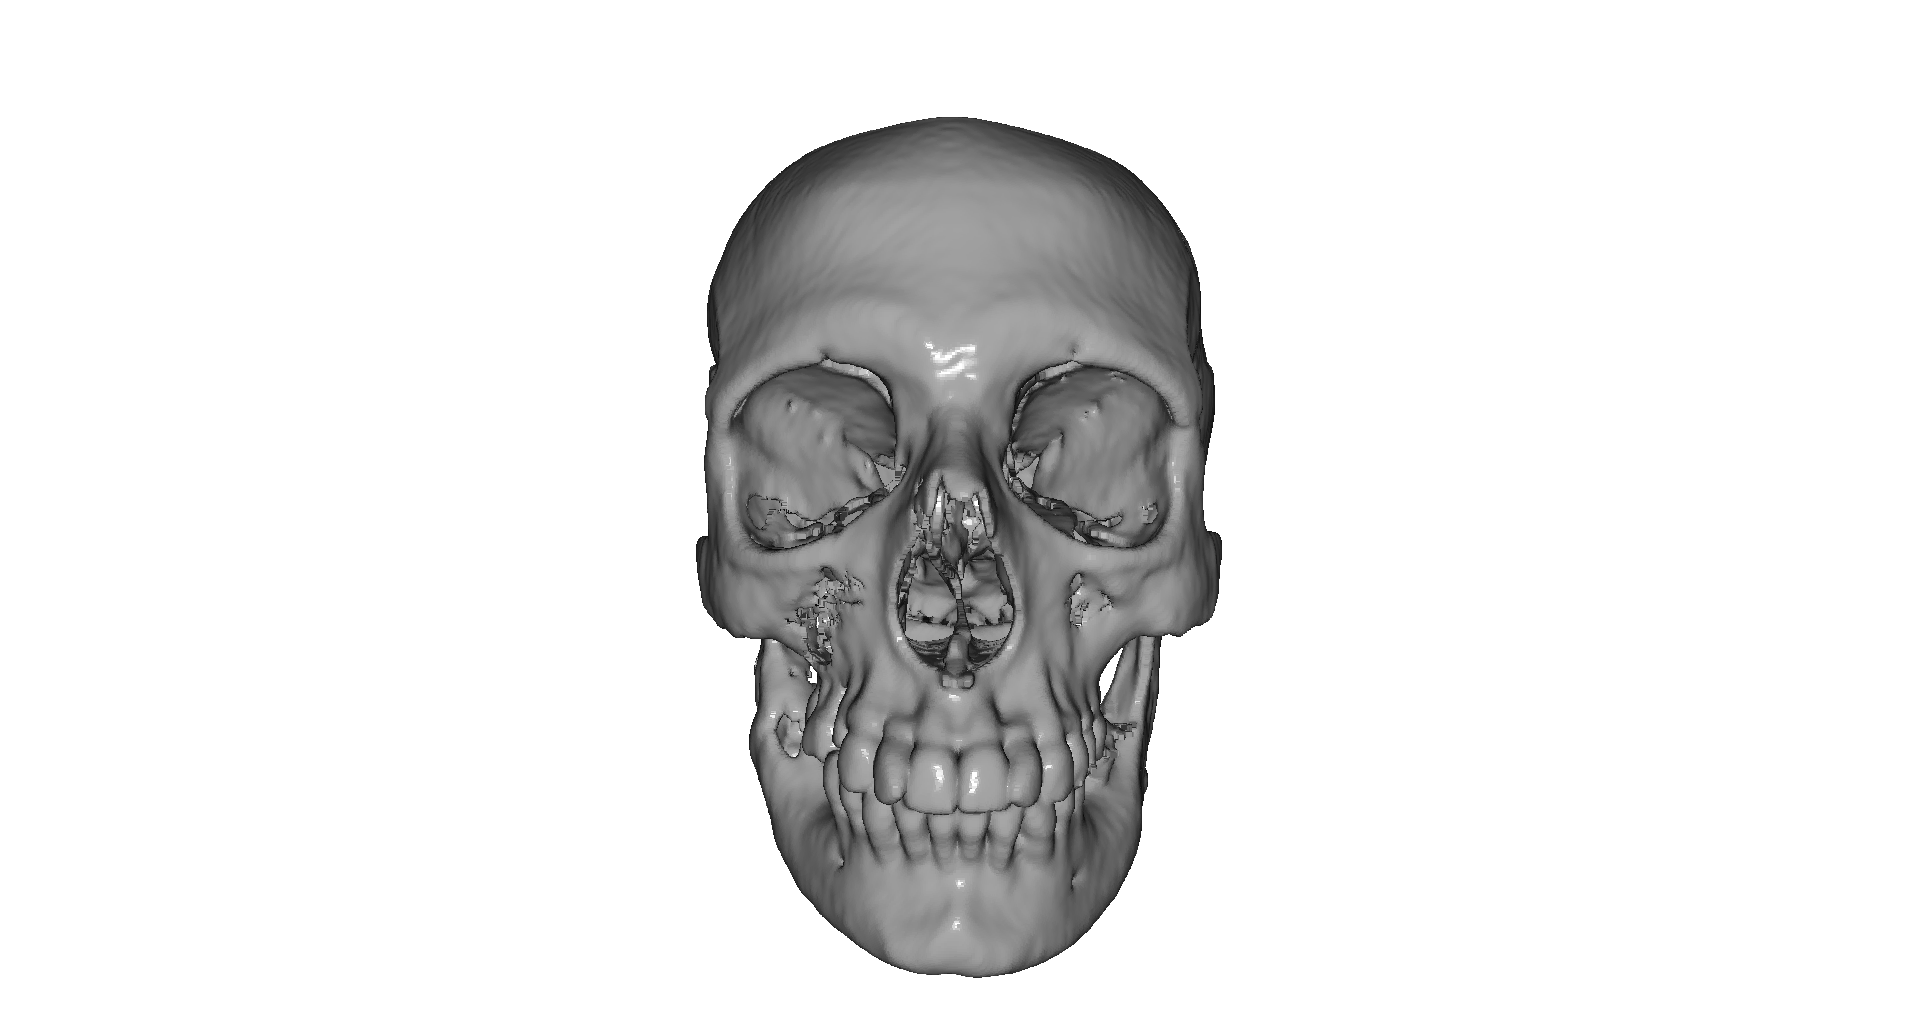
\includegraphics[width=\textwidth]{imagenes/chapter4/Craneo12018377.png}
  \end{subfigure}
  \begin{subfigure}[b]{0.40\textwidth}
  \centering 
  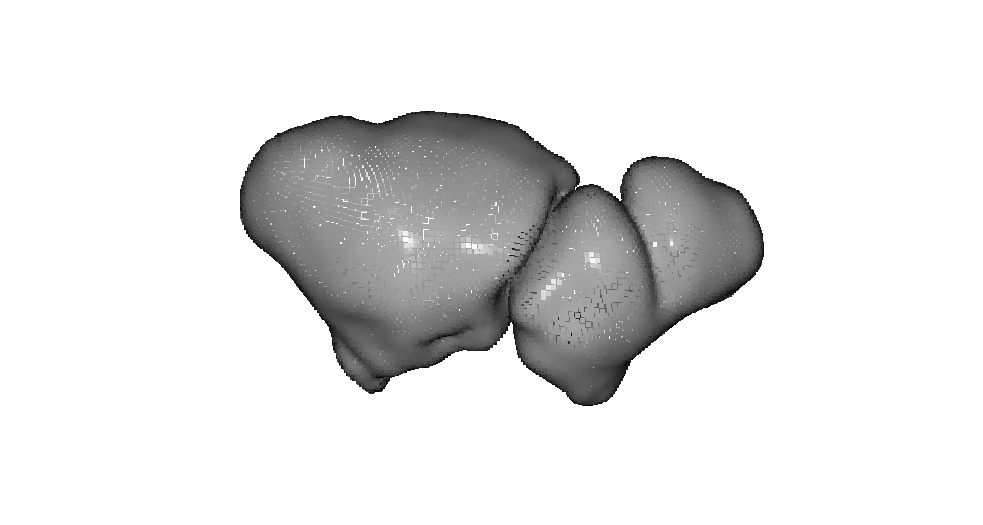
\includegraphics[width=\textwidth]{imagenes/chapter4/SenoFrontal100205.png}
  \end{subfigure}

  \begin{subfigure}[b]{0.40\textwidth}
  \centering 
  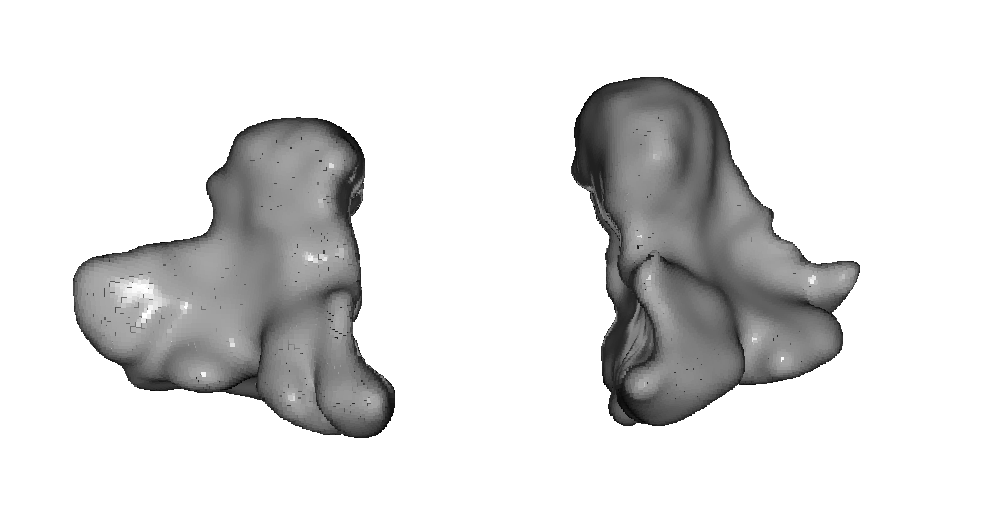
\includegraphics[width=\textwidth]{imagenes/chapter4/Maxilar100205.png}
  \end{subfigure}
  \begin{subfigure}[b]{0.40\textwidth}
  \centering 
  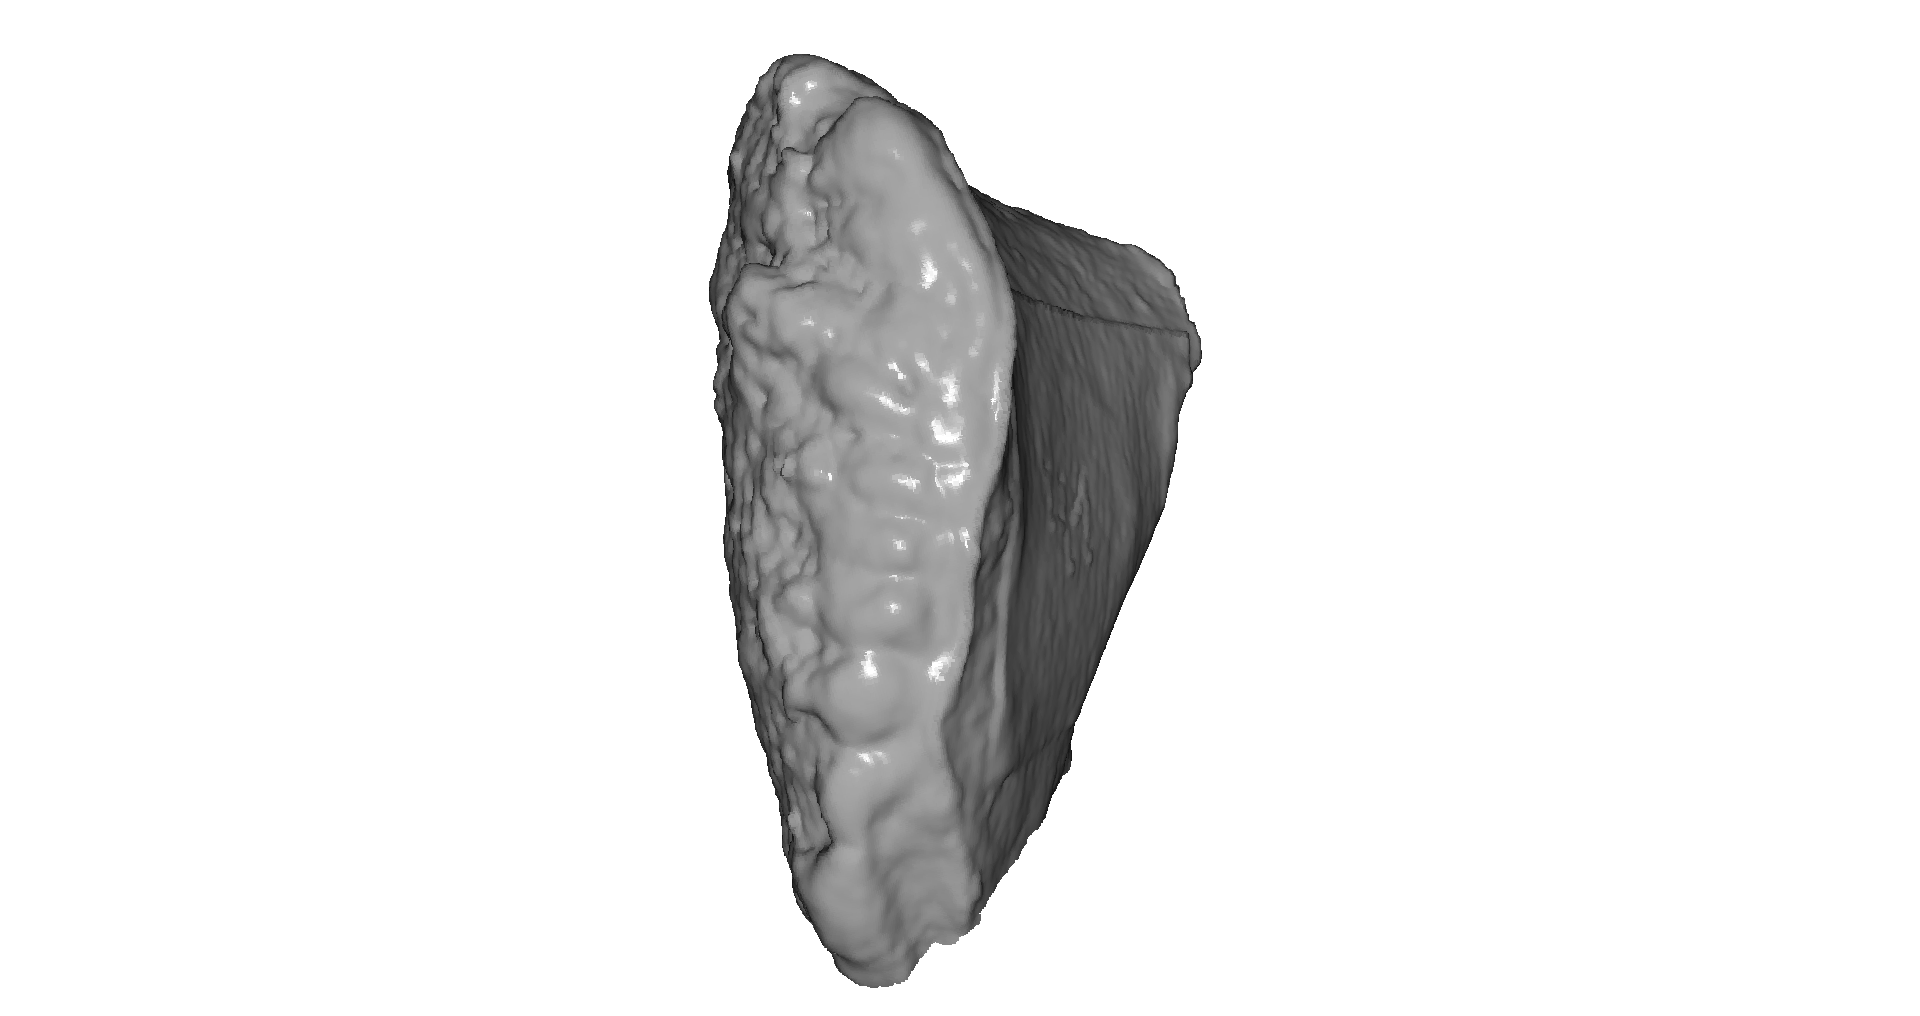
\includegraphics[width=\textwidth]{imagenes/chapter4/PubisDch.png}
  \end{subfigure}
  \caption[Ejemplo de nuestras imágenes médicas]{Ejemplo de nuestras imágenes médicas.
  Arriba a la izquierda tenemos un cráneo y a su derecha un seno frontal. 
  Abajo a la izquierda tenemos un maxilar y a su derecha el pubis derecho.}
  \label{fig:OurDataExample}
\end{figure}


\section{Métodos}
Como se pudo observar en la Sección \ref{sec:EstadoDelArte}, actualmente hay una 
tendencia, justificada, a los métodos de DL. No obstante, se tuvo 
que descartar todos los métodos que tuvieran en cuenta información de textura, 
cosa que no existe en los volúmenes médicos habituales. Además, necesitamos 
información perceptual de la imagen en su totalidad y no de regiones locales 
específicas. Ambas características son dificultades añadidas a la hora 
de resolver el problema. La primera restringe el problema 
a la estimación de calidad de las estructuras en la imagen, eliminando la 
percepción de calidad por contraste y saturación. La segunda incrementa 
la complejidad computacional.

\subsection{Zhang et al\cite{NR3DQA}}
\label{sec:NR3DQA}
Antes de probar directamente con modelos de DL, se experimentó con un método de 
ML basado en la extracción de características de escena y entrenamiento de un 
modelo de vectores soporte para la regresión. Para ello necesitamos definir 
que tipo de características queremos extraer. 

Zhang et al\cite{NR3DQA} proponen utilizar características geométricas y de 
color. Para la primera, extraen la curvatura\eqref{eq:Curvatura}, 
anisotropia\eqref{eq:Anisotropia}, linealidad\eqref{eq:Linealidad}, 
planaridad\eqref{eq:Planaridad} y esfericidad\eqref{eq:Esfericidad} de los puntos. 
Estas características se pueden extraer del vecindario 
de un punto por medio de la matriz de covarianza y los valores singulares. 
Las fórmulas que las definen son: 
\begin{equation}
  Cur(p_i) = \frac{\lambda_3}{\lambda_1 + \lambda_2 + \lambda_3}
  \label{eq:Curvatura}
\end{equation}
\begin{equation}
  Ani(p_i) = \frac{\lambda_1 - \lambda_3}{\lambda_1}
  \label{eq:Anisotropia}
\end{equation}
\begin{equation}
  Lin(p_i) = \frac{\lambda_1 - \lambda_2}{\lambda_1}
  \label{eq:Linealidad}
\end{equation}
\begin{equation}
  Pla(p_i) = \frac{\lambda_2 - \lambda_3}{\lambda_1}
  \label{eq:Planaridad}
\end{equation}
\begin{equation}
  Sph(p_i) = \frac{\lambda_3}{\lambda_1}
  \label{eq:Esfericidad}
\end{equation}
Donde $\lambda_1$, $\lambda_2$ y $\lambda_3$ se refieren a los correspondientes 
valores singulares. Para la extracción de las características de color, primeramente 
convierten el espacio de color RGB en el espacio LAB mediante los siguientes 
pasos de transformación: 
\begin{equation}
  \begin{bmatrix} 
    X \\ Y \\ Z 
  \end{bmatrix}  = 
  \begin{bmatrix}
    2.7688 & 1.7517 & 1.1301 \\ 
    1.0000 & 4.5906 & 0.0601 \\ 
    0 & 0.0565 & 5.5942 
  \end{bmatrix} = 
  \begin{bmatrix}
    R \\ G \\ B 
  \end{bmatrix} 
  \label{eq:ScaleXYZ}
\end{equation}
\begin{equation}
\begin{cases}
  L &= 116f\left(\frac{Y}{Y_n}\right) - 16 \\ 
  A &= 500\left( f\left(\frac{X}{X_n}\right) - f\left(\frac{Y}{Y_n}\right) \right) \\ 
  B &= 200\left( f\left(\frac{Y}{Y_n}\right) - f\left(\frac{Z}{Z_n}\right)\right) 
\end{cases}
  \label{eq:LABTransform}
\end{equation}
Donde R, G y B son los correspondientes canales RGB de color. La función que 
determina la transformación final viene descrita por \eqref{eq:LABfun}: 
\begin{equation}
  f(t) = \begin{cases} \sqrt[3]{t} & \textrm{sí}\; t > \sigma^3 \\ 
    \frac{t}{3\sigma^2} + \frac{4}{29},& \textrm{en cualquier otro caso.}
         \end{cases}  
  \label{eq:LABfun}
\end{equation}
Donde $\sigma = \frac{6}{29}$.
Sin embargo, en el caso de las imágenes médicas estas características deben 
ser descartadas, dado que el color existente al visualizar las nubes de puntos 
médicas no son más que un valor sintético añadido previamente que permite 
una visualización más agradable de las mismas. 
Además, estiman la entropía de cada una de las características 
ya que argumentan que existe una alta correlación entre la 
entropía y la distorsión por cuantización. 
Por último, a las características geométricas se les calcula 
la distancia a las distribuciones gaussiana y gamma tras observarse 
que la distribución de estas se veía afectada por la intensidad 
de las distorsiones. 

Para cada tipo de característica, se utiliza el valor medio y la desviación típica 
obtenida para cada punto de la nube de punto. A continuación, sobre estas medidas, 
para el conjunto de datos de entrenamiento se normaliza como \eqref{eq:MeanNorm}.
Donde F es la característica extraída y C una pequeña constante para la 
estabilidad numérica. 
\begin{equation} 
  \hat F = \frac{F-mean(F)}{std(F) + C}
  \label{eq:MeanNorm}
\end{equation}


\subsection{VQA-PC}
Zhang et al\cite{VQA-PC} propusieron un modelo de estimación de calidad de nubes 
de puntos utilizando proyecciones 2D de diferentes perspectivas. 
Observaron que los métodos que trabajan directamente sobre la nube de puntos tienen
una elevada dificultad computacional, sin suponer una mejora excesiva, y que 
deben todavía que madurar en el campo dado la alta complejidad de las nubes de puntos.
Por ello proponen utilizar proyección multi-vista. No obstante, argumentaron que 
los métodos anteriores de proyección se basan en la hipótesis de que los humanos 
percibimos la calidad de modelos 3D desde una perspectiva estática, cosa que no 
es cierta en la práctica dado que los objetos 3D permiten operaciones geométricas 
de rotación y escalado.
Y por ello, proponen unificar la percepción estática con la dinámica tratando 
a las proyecciones como vídeos.

De esta forma, se puede extraer características espaciales y temporales, como 
discutido en la Sección \ref{sec:VideoCNN}, utilizando redes convolucionales 
adaptadas a vídeos, de la familia \emph{SlowFast}\cite{SlowFastNetworks}.
Siguiendo la motivación de que las deformaciones geométricas no deseadas se presentan 
de forma abrupta según la perspectiva, ver Figura \ref{fig:ViewPoint}, y que 
incluso se pueden observar incoherencias entre perspectivas adyacentes
utilizaron 4 ejes de rotación: vertical, horizontal, diagonal derecha 
y diagonal izquierda. Para cada eje se genera un total de 30 \emph{frames}, 
en total habrá 120, ver Figura \ref{fig:VQARotation}. El ángulo de rotación es de 12 grados para todos los casos. 
Terminando la rotación de un eje en la misma posición inicial. 
A continuación se extraen características temporales del vídeo, que es posible 
generar a partir de cada \emph{frame} de los distintos ejes de rotación encadenados
secuencialmente de forma ordenada, y se elige 1 \emph{frame} de cada 
eje de rotación para representar la información espacial. Por último, 
tenemos que aprender una función de interacción entre los dos vectores característicos 
extraídos. Proponen concatenar los vectores y aprender una función por 
medio de una capa totalmente conectada utilizando el MSE.

\begin{figure}
  \begin{center}
    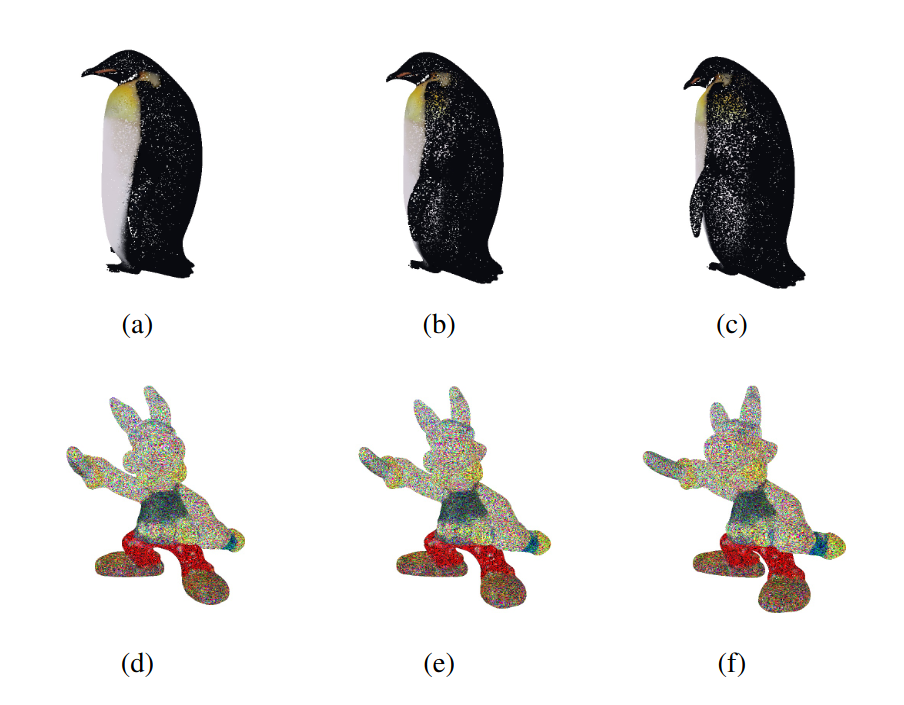
\includegraphics[width=0.75\textwidth]{imagenes/chapter4/ViewPoint}
  \end{center}
  \caption[Ejemplo de distorsiones que se presentan según la perspectiva]{
  Ejemplo de distorsiones que se presentan según la perspectiva.
Vemos que al girar el pingüino se empieza a observar un bajo número de puntos en su 
lateral izquierdo, permitiendo verse a través de él. De forma similar, 
en la imagen de abajo se ve cierta deformación de la cabeza.}
  \label{fig:ViewPoint}
\end{figure}

\begin{figure}
  \begin{center}
    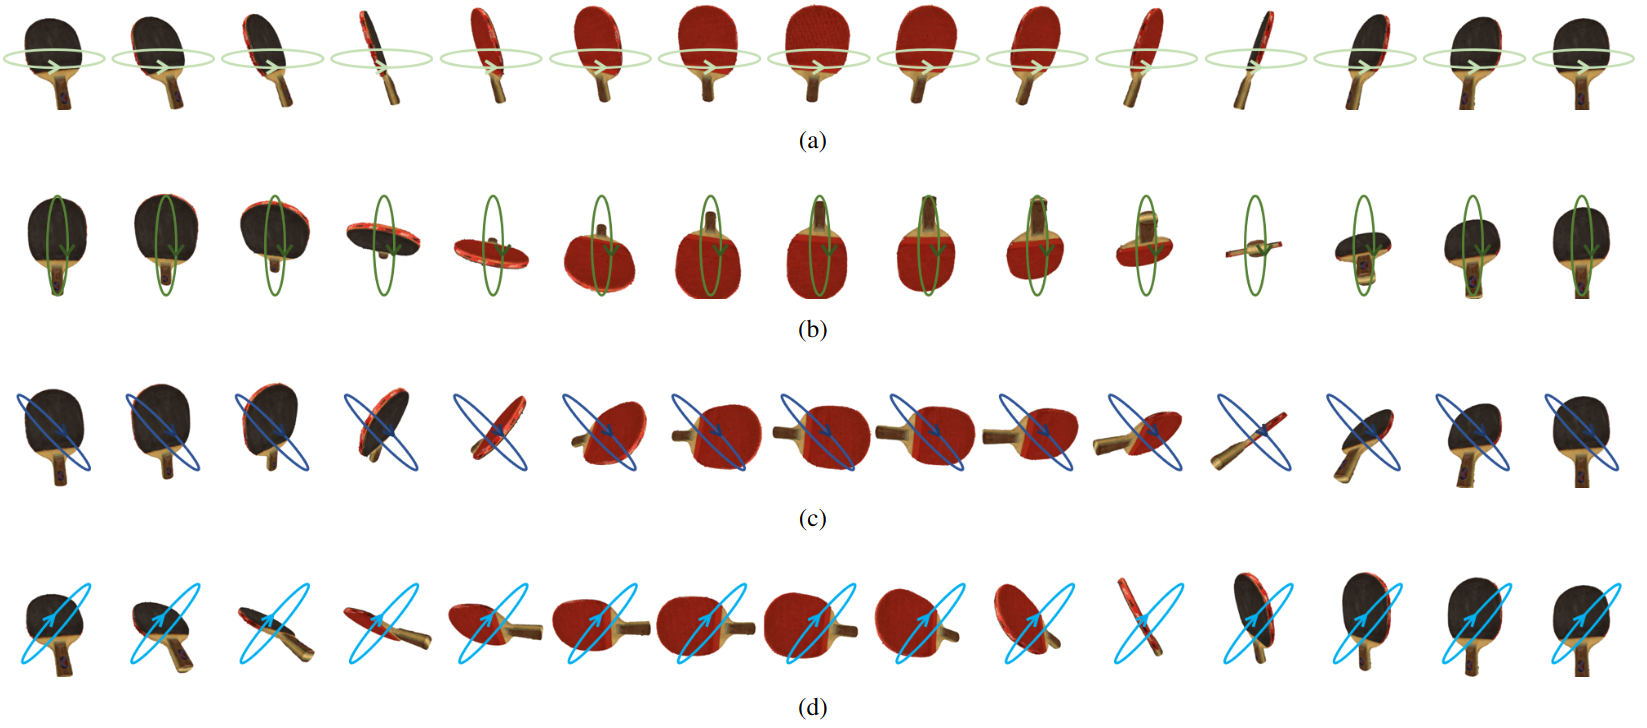
\includegraphics[width=\textwidth]{imagenes/chapter4/VQARotation}
  \end{center}
  \caption[Ejemplo de las rotaciones que utiliza el modelo VQA-PC\cite{VQA-PC}.]
  {Ejemplo de las rotaciones que utiliza el modelo VQA-PC\cite{VQA-PC}.
  Se observa que el final de cualquier eje de rotación es la posición inicial, 
permitiendo así unir suavemente una secuencia de imágenes encadenada de los ejes 
que genere un vídeo de rotación utilizado luego para la estimación.}
  \label{fig:VQARotation}
\end{figure}

Para realizar la secuencia de vídeo, necesitamos realizar correctamente 
el conjunto de rotaciones descritos por las siguientes ecuaciones: 
\begin{equation}
  \theta_A = 
\begin{cases}
\begin{aligned}
   X_\alpha^2 + Y_\alpha^2 & = R^2 \\ 
    Z_\alpha & = 0 
\end{aligned}
\end{cases}
\label{eq:RotationA}
\end{equation}

\begin{equation}
  \theta_B = 
\begin{cases}
\begin{aligned}
   Y_\alpha^2 + Z_\alpha^2 & = R^2 \\ 
    X_\alpha & = 0 
\end{aligned}
\end{cases}
\label{eq:RotationB}
\end{equation}

\begin{equation}
  \theta_C = 
\begin{cases}
\begin{aligned}
   X_\alpha^2 + Y_\alpha^2 + Z_\alpha^2 & = R^2 \\ 
    X_\alpha + Z_\alpha & = 0 
\end{aligned}
\end{cases}
\label{eq:RotationC}
\end{equation}

\begin{equation}
  \theta_D = 
\begin{cases}
\begin{aligned}
   X_\alpha^2 + Y_\alpha^2 + Z_\alpha^2 & = R^2 \\ 
    X_\alpha - Z_\alpha & = 0 
\end{aligned}
\end{cases}
\label{eq:RotationD}
\end{equation}

Y para llevar a cabo la rotación debemos calcular el punto medio de la nube 
de puntos por medio de la siguiente ecuación \eqref{eq:PuntoMedio}:
\begin{equation}
  O_\sigma = \frac{1}{N}\sum_{n=1}^N \sigma_n
  \label{eq:PuntoMedio}
\end{equation}
Donde el $O_\sigma$ representa la coordenada (X,Y,Z) del centro medio de la 
nube de punto, y $\sigma_n$ representa la coordenada del punto $n$-ésimo punto. 
Utilizando ese centro, aplicamos las ecuaciones \eqref{eq:RotationA} a \eqref{eq:RotationD}.

Para extraer las características espaciales empleamos un modelo pre-entrenado, 
en concreto se investigaron variaciones de arquitecturas ResNet\cite{ResNet}. Una 
familia de redes residuales, que en su momento resolvieron el problema 
del estancamiento en el entrenamiento de redes neuronales profundas debido 
a la degradación del gradiente. El único modelo al que optimizaremos sus pesos es 
ResNet, el modelo de extracción temporal solo es un paso previo.

\begin{figure}[H]
  \begin{center}
    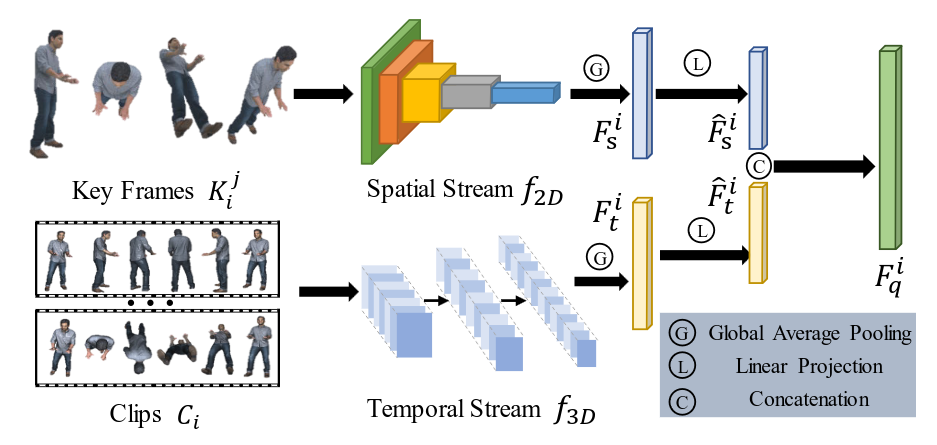
\includegraphics[width=0.60\textwidth]{imagenes/chapter4/PipelineCompleto}
  \end{center}
  \caption{Ejemplo detallado de las etapas del método de VQA-PC}
  \label{fig:VQAPipeline}
\end{figure}


% %
\chapter{Implementación y Experimentos} 
\section{Detalles Técnicos de Implementación} 
\section{Distorsiones}
\section{Experimentos} 

%
%\input{capitulos/06_Implementacion}
%
%\input{capitulos/07_Pruebas}
%
\chapter{Conclusiones y Trabajos Futuros}
La estimación de la calidad de imágenes (IQA) es un problema esencial a la hora 
de optimizar el formato y visualización de la información, además es de 
suma importancia para el ámbito biomédico. 
Este TFG aborda la obtención de una métrica de estimación de calidad capaz de evaluar 
representaciones 3D sin referencia, en concreto nubes de puntos, del ámbito biomédico para poder asistir 
en la mejora de los algoritmos de reconstrucción y visualización de dichos objetos. 

En primer lugar, se realizó un estudio de la literatura relativa a la estimación de calidad 
de imágenes 2D, desde los métodos basados en extracción de características de escenas naturales y modelos de ML, 
hasta la extracción automática con DL. 
A continuación, se estudió el uso de estos y otros métodos sobre imágenes médicas 2D.
Posteriormente se analizó el estado del arte de métodos dedicados a representaciones tridimensionales. 
Se observa un salto en complejidad teórica y computacional al tratarse de problemas 
en tres dimensiones. 
Por último, se concluye que no existe hasta el momento 
otra investigación que haya tomado el enfoque novedoso de estimar la calidad de 
reconstrucciones biomédicas 3D. 

Ante la falta de propuestas específicas, el trabajo parte de la implementación 
de métodos relevantes del estado del arte de estimación de calidad de objetos 3D, 
tanto desde la perspectiva de métodos tradicionales (ML, en donde la extracción 
de características y la clasificación son etapas independientes) como de métodos 
\emph{end-to-end} DL. El primero hace uso de características 
extraídas manualmente utilizando conocimiento humano sobre el sistema visual humano (HVS), 
como fenómenos de planaridad, esfericidad, anisotropía, curvatura, linealidad y consistencia de 
colores de las nubes de puntos, que luego se utilizan para estimar una regresión por 
SVM. En cuanto a modelos basados en DL, se utilizó un modelo capaz de extraer 
información estática y dinámica de nubes de puntos haciendo uso de múltiples 
proyecciones 2D y de un vídeo del objeto 3D rotando. De esta forma, podemos  
simular el HVS. En ambos casos se proponen ajustes y pequeñas mejoras basadas 
en recientes publicaciones y se comparan los resultados con la propuesta original. 

Para la validación sobre un conjunto de datos médicos fue necesaria la creación 
de un conjunto de datos sintético debido a la no existencia de un conjunto de 
datos públicos para este análisis. Para ello se estudiaron y se fabricaron las distorsiones más 
comunes del ámbito biomédico con respecto a las representaciones 3D. 
Para evitar la problemática logística del etiquetado a través de la 
evaluación humana sobre el dataset sintético, 
fue necesario estudiar el problema IQA con referencia y hacer uso de las métricas 
más empleadas. Dichas métricas demonstraron una alta correlación con el HVS, 
justificando así su uso para generar etiquetas artificiales.
Se generaron un total de 385 representaciones médicas 3D distorsionadas, 11 nubes de puntos 
base, 5 distorsiones a 7 niveles cada una. En las distorsiones se simula 
tanto errores de transmisión, compresión como el movimiento del paciente.

Como primera conclusión de nuestra experimentación base, 
siguiendo la tendencia del estado del arte, el modelo DL sale exitoso en la 
comparativa sobre objetos 3D genéricos. Dicha conclusión es consecuencia 
de lograr replicar satisfactoriamente los resultados de los métodos estudiados 
sobre los conjuntos de datos públicos.
A continuación, se observa que el modelo adaptado de ML (NR3DQA) demuestra no 
ser capaz de determinar con calidad el nivel de distorsiones de las imágenes médicas. 
Sin embargo, el modelo basado en DL (VQA-PC) consigue resultados aceptables con 
una correlación media del 71\%.
Finalmente, se aplican mejoras a los métodos 
y se concluye que, tras entrenar con datos sintéticos de distorsiones similares y 
diversas nubes de puntos, se obtiene una mejora considerable en el modelo basado en DL. 
En concreto, se alcanza una alta correlación (88\%) utilizando la aproximación F2 
(fusión por convolución).

Por lo tanto, se concluye que se han completado satisfactoriamente los objetivos 
planteados, determinando la posibilidad de resolución del problema adaptado 
al ámbito biomédico y abriendo puertas a futuras investigaciones. 
Todo el código se encuentra disponible en el siguiente repositorio de 
GitHub \url{https://github.com/CodeBoy-source/TFG_NRPCQA},
a excepción de las imágenes médicas ya que son datos confidenciales.

Siendo un proyecto en una nueva línea de investigación, existen varias ampliaciones 
lógicas que se pueden realizar a este proyecto. Por un lado, se podría 
obtener una etiqueta manual con un experimento de evaluación, según los estándares, para 
obtener una opinión media de calidad (MOS) y volver a validar los resultados obtenidos
entre los distintos modelos. Así como utilizar ese conjunto de MOS manual sobre imágenes médicas 
para normalizar las etiquetas sintéticas como lo hacen en la publicación original~\cite{ResSCNN}, 
en donde se parte de un conjunto pequeño extraído manualmente para obtener uno sintético varias 
veces más grande. También, para mejorar el método propuesto, se podría permitir 
que los pesos del modelo utilizado para la extracción de características 
del vídeo fueran alterados en vez de ser solamente un paso previo, de extracción. 
De esta forma se podría guiar el modelo a buscar nuevas características temporales.  
Además, se podría buscar simular las distorsiones 
sobre el conjunto de imágenes 2D generadas tras el examen en vez de hacerlo 
sobre la representación 3D final, teniendo así datos más realistas. 

Por otro lado, se pueden explorar otros métodos que procesen modelos 3D directamente, 
o que hagan uso de proyecciones y de la nube de puntos simultáneamente, como en MM-PCQA~\cite{MM-PCQA}.
Actualmente, ha crecido el número de publicaciones de adaptaciones de PointNet~\cite{PointNet} y 
PointNet++~\cite{PointNet++} para resolver distintos problemas de nubes de puntos, 
por lo que quizás se podría adaptar para la resolución de este problema, como 
el método de ResSCNN~\cite{ResSCNN} y evitar así 
la pérdida de información al proyectar en 2D.

%
%
\nocite{*}
% \bibliography{bibliografia/bibliografia}\addcontentsline{toc}{chapter}{Bibliografía}
% \bibliographystyle{unsrturl}
\newpage
\chapter{Bibliografía}
\printbibliography[heading=none]
\appendix
\chapter*{}
\section*{Búsquedas en Scopus}
\label{subs:Scopus}
\begin{enumerate}
\item 
{\footnotesize
  \textbf{Inteligencia artificial en imágenes médicas}\\\hfill
 TITLE-ABS-KEY ((deep AND learning) OR (machine AND learning) 
 OR (artificial AND intelligence) OR (computer AND vision) 
 OR (soft AND computing) AND ((biomedical AND image AND analysis) 
 OR (medical AND imaging) OR (medical AND image AND analysis))) 
 AND (LIMIT-TO (SUBJAREA , ``COMP'') OR LIMIT-TO (SUBJAREA , ``MEDI'') 
OR LIMIT-TO (SUBJAREA , ``ENGI''))
}
{\footnotesize
 \item \textbf{Inteligencia artificial en nubes de puntos}\\\hfill
 TITLE-ABS-KEY ((deep AND learning) OR (machine AND learning) OR (artificial AND intelligence) OR (computer AND vision) OR (soft AND computing) AND ((point AND cloud) OR (3d OR tridimensional))) AND (LIMIT-TO (SUBJAREA , ``COMP'') OR LIMIT-TO (SUBJAREA , ``MEDI'') OR LIMIT-TO (SUBJAREA , ``ENGI''))
}
{\footnotesize
 \item \textbf{Estimación de calidad en imágenes médicas}\\\hfill
 TITLE-ABS-KEY ((deep AND learning) OR (machine AND learning) OR (artificial AND intelligence) OR (computer AND vision) OR (soft AND computing) AND ((biomedical AND image AND analysis) OR (medical AND imaging) OR (medical AND image AND analysis)) AND ((quality AND assessment) OR (quality AND estimation) OR (mos))) AND (LIMIT-TO (SUBJAREA , ``COMP'') OR LIMIT-TO (SUBJAREA , ``MEDI'') OR LIMIT-TO (SUBJAREA , ``ENGI'')) 
}
{\footnotesize
 \item \textbf{Estimación de calidad en nubes de puntos}\\\hfill
 TITLE-ABS-KEY ((deep AND learning) OR (machine AND learning) OR (artificial AND intelligence) OR (computer AND vision) OR (soft AND computing) AND ((point AND cloud) OR (3d OR tridimensional)) AND ((quality AND assessment) OR (quality AND estimation) OR (mos))) AND (LIMIT-TO (SUBJAREA , ``COMP'') OR LIMIT-TO (SUBJAREA , ``MEDI'') OR LIMIT-TO (SUBJAREA , ``ENGI''))
}
{\footnotesize
 \item \textbf{Estimación de calidad de imágenes médicas 3D}\\\hfill
 TITLE-ABS-KEY ((deep AND learning) OR (machine AND learning) OR (artificial AND intelligence) OR (computer AND vision) OR (soft AND computing) AND ((biomedical OR medical OR medicine)) AND ((point AND cloud) OR (3d OR tridimensional)) AND ((quality AND assessment) OR (quality AND estimation) OR (mos))) AND (LIMIT-TO (SUBJAREA , ``COMP'') OR LIMIT-TO (SUBJAREA , ``MEDI'') OR LIMIT-TO (SUBJAREA , ``ENGI''))
}
\end{enumerate}


\section*{Detalles Técnicos de Implementación} 
\label{sec:Implementacion}
Este proyecto ha sido realizado mayoritariamente con el lenguaje de programación Python, 
debido a que casi todos los modelos analizados estaban descritos en el mismo.
No obstante, para la distorsión por compresión \emph{octree}~\cite{OctreeCompression}, 
se hizo uso de la librería PCL~\cite{PCL} en el lenguaje C++.

Para el desarrollo y ejecución de los modelos fue necesario el uso de
la librería de DL Pytorch junto con las librerías CUDA de para poder ejecutar 
los modelos en las tarjetas gráficas de NVIDIA. Para los cálculos numéricos y 
el manejo de datos se utilizaron Numpy y Polars, librería similar a Pandas 
pero basada en Rust, más eficiente y fácilmente paralelizable. Además, para el
cálculo de las métricas se utilizó la librería scikit-learn.
Para la visualización y fácil manipulación de las nubes de puntos se hizo uso 
de la librería de Open3D~\cite{Open3D} y Pyntcloud~\cite{Pyntcloud}.
Se ha gestionado el uso de estas librerías y todas sus dependencias tanto en entornos virtuales 
de python como en entornos creados por cuadernos jupyter de Colab.

Para el control de versiones del proyecto se utilizó de forma conjunta Git, GitHub
y la gestión de versiones de Google Drive. El repositorio de este proyecto se 
puede acceder por la siguiente dirección: \url{https://github.com/CodeBoy-source/TFG_NRPCQA}.
Este mismo, se encuentra dividido en un conjunto de carpetas: 
\begin{itemize}
  \item \textbf{Distort}, donde se encuentra todo lo necesario para la generación 
    de las distorsiones médicas dado un directorio de archivos \code{.ply}. 
    A su vez, posee lo necesario para la generación de las etiquetas sintéticas 
    de calidad, ver Sección \ref{sec:DatosSinteticos}.
  \item \textbf{Document}, donde se encuentra la documentación del proyecto, 
    incluyendo a este documento. 
  \item \textbf{NR3DQA}, implementación y experimentos del método propuesto 
    por Zhang et al\cite{NR3DQA}.
  \item \textbf{Utils}, conjunto de scripts de python para la realización de distintas 
    tareas. Como por ejemplo la lectura de un directorio DICOM, la visualización 
    de una o un conjunto de nubes de puntos y división del conjunto de datos LS-SJTU-PCQA\cite{ResSCNN}.
  \item \textbf{VQA\_PC}, implementación de la variante VQA-PC\cite{VQA-PC} para 
    la estimación de calidad de nubes de puntos y las modificaciones pertinentes 
    sobre los métodos de fusión de características mencionados en \cite{EnsemblePCQA}. 
\end{itemize}
\subsection*{Generación de un conjunto de datos de imágenes médicas.}
Los datos se encuentran en una carpeta del servicio UGRDrive, que provee almacenamiento 
en la nube para investigadores. Los modelos mencionados en la Sección \ref{sec:OurData} 
se encuentran dentro de una carpeta numerada por cada individuo con los ficheros 
necesarios para el desarrollo del proyecto. Se incluyen incluso algunos directorios 
DICOM enteros por si fuera necesario generar más datos a partir de la segmentación 
manual. 

Se desarrolló un fichero \code{gen_distortions.py} que automáticamente genera 
un conjunto de distorsiones dado un directorio de entrada con archivos \code{.ply} y los 
guarda en un directorio de salida especificado por argumento. Para ello se hace 
uso de las distorsiones realizadas con Open3D~\cite{Open3D} 
con el archivo del directorio \code{utils/distortions.py} y un ejecutable hecho 
con C++ y Makefile para la distorsión \emph{octree}. A continuación, 
podemos generar las etiquetas sintéticas con \code{get_metrics.py}, que dado un 
directorio de entrada con las nubes de referencia y uno con las distorsiones, 
genera un \code{.csv} con las etiquetas sintéticas generadas con las métricas 
del estado del arte de los métodos FR-PCQA. Para ello se hace uso de un 
software desarrollado con PCL~\cite{PCL} y el archivo del directorio \code{utils/metrics.py}. 

\subsubsection*{Preprocesado de datos}
El único preprocesado que sufren los datos iniciales es el centrado de la nube 
de puntos sobre los ejes, paso previo a la rotación. Y la reducción de puntos 
anormales por medio de un análisis de consistencia estadística del vecindario,
eliminado así puntos aislados y ruido. 

El proceso es muy sencillo, dado el vecindario de un punto definido por sus 
K vecinos más cercanos, calculamos la desviación típica y la media de sus atributos 
geométricos y eliminamos aquellos que sobrepasen un umbral determinado. 
En nuestro caso utilizamos K = 32 y el umbral a 5 desviaciones típicas. Para 
ello se puede utilizar \code{Utils/std_remove.py}.

\subsection*{Distorsiones}
\label{sec:DatosSinteticos}
\subsubsection*{Ruido Gaussiano} 
Para la generación del ruido gaussiano, que en este caso simula posibles 
errores de transmisión y generación, se hizo uso de la función que se denomina
\code{gaussian_geometric_shift}. 
Esa función toma como entrada 
una nube de punto y un nivel de intensidad. La salida es una nube de puntos que, 
a cada punto, se le ha aplicado un desplazamiento geométrico, cuyo valor 
viene sacado de una distribución gaussiana de media 0 y desviación típica 
basada en el nivel de intensidad. Ese nivel de intensidad es un porcentaje 
de la caja que recubre la nube de puntos, en inglés \emph{bounding box}.
Los valores utilizados son: 0.15\%, 0.2\%, 0.25\%, 0.30\%, 0.35\%, 0.4\% y 0.5\%
del \emph{bounding box}.
\subsubsection*{Compresión \emph{Octree}}
En la carpeta \code{Distort/octree/} tenemos la implementación en C++ de esta 
distorsión, en concreto en \code{point_cloud_compression.cpp}. Se facilita 
un \code{CMakeLists.txt} para la generación del ejecutable con el comando 
\code{cmake}. Recibe de entrada la ruta a la nube de puntos de referencia, 
la resolución de compresión \emph{octree} y el directorio de salida. 
La resolución se refiere al tamaño de los vóxeles más pequeños en el nivel más 
bajo del \emph{octree}. Cuanto más pequeña sea la resolución, mayor será la precisión 
en la representación de los detalles espaciales. 
La profundidad del \emph{octree} depende tanto de la resolución como de la dimensión 
espacial de la nube de puntos, ya que determina cuántos niveles de subdivisión 
serán necesarios para cubrir toda el área de la nube de puntos con la resolución 
especificada. Parar más detalles repasar \ref{sec:Distorsiones}. 
Se facilita también la entrada de dos parámetros adicionales para obtener 
las estadísticas de compresión y otro para visualizar el resultado final del 
decodificador. Las resoluciones son: 0.4, 0.5, 0.6, 0.7, 0.8, 0.9 y 1.0.
\subsubsection*{Submuestreo aleatorio}
Esta distorsión también simula pérdida de datos en momentos de transmisión o 
generación de la nube de puntos. Incluso se podría considerar una forma de 
compresión. El método es trivial, dado un nivel de intensidad en el intervalo 
0--1, que representa el porcentaje de reducción, se procede a elegir de forma 
aleatoria puntos a ser eliminados hasta alcanzar ese porcentaje. Los valores 
de reducción son: 10\%, 20\%, 30\%, 40\%, 50\%, 60\% y 70\%.
\subsubsection*{Rotación y Movimiento Local}
Esta distorsión simula el movimiento del paciente durante el examen médico. 
Para ello hemos elegido de forma aleatoria una región local de la nube de punto, 
cuyo tamaño corresponde al 20\% del lado más grande del \emph{bounding box}, y 
le hemos aplicado un desplazamiento geométrico que equivale al 1\% del lado 
más largo. Los niveles de intensidad en este caso se refieren a cuántas veces 
se repiten el proceso de seleccionado y desplazamiento local. 
La rotación es simplemente una extensión de la anterior, reflejando otro tipo de movimiento, 
donde la selección se rota 15 grados sobre el eje X. Se aplican niveles del 1 al 7 en intervalos de 1.
\subsection*{Detalles técnicos de la experimentación} 
\label{sec:TrainML}
La estimación de calidad del modelo DL se puede realizar invocando al script \code{train.py} de la carpeta \code{VQA_PC},
el cual recibe múltiples parámetros de entrada: se define el modelo a utilizar, 
se define el método de fusión de características, el ratio de aprendizaje base,
la frecuencia en la que decrece, dónde están los datos, etc. Ese script nos 
provee las métricas resultantes de haber realizado validación cruzada, 
ver Sección \ref{sec:Validation}, 
para un conjunto de datos con los parámetros establecidos. 
Para realizar una prueba desde un modelo pre-entrenado disponemos del script 
\code{test.py}, al igual que el anterior recibe parámetros similares de entrada.
Si se prefiere, se pone a disposición un cuaderno de jupyter con la implementación 
bajo la librería \emph{fastai}~\cite{fastai}.
Mientras que para el modelo ML, disponemos de los scripts de extracción 
de características y los scripts necesario para la evaluación del 
modelo sobre SJTU\cite{SJTU} o WPC\cite{WPC1, WPC2} en la carpeta \code{NR3DQA}.

Para la ejecución se utilizaron dos sistemas distintos. En las pruebas de alta 
carga de CPU, como la generación de las distorsiones y las proyecciones, 
se utilizó un ordenador portátil ASUS FX505DY con una CPU AMD Ryzen 5 
3550H, 16 GB de RAM DDR4 y una AMD Radeon RX560X que posee 4GB de VRAM. Ya 
que, en contra del Intel Xeon CPU E5-2699 2.2GHZ de 2 vCPUs (hebras virtuales), 
nos permite utilizar hasta 4 núcleos, para un total de 8 hebras en paralelo. 
Sin embargo, dado la necesidad de una gran cantidad VRAM, aproximadamente 13GB, 
se utilizó los servicios de Colab para la ejecución del entrenamiento del modelo. 
En este, disponemos de una NVIDIA Tesla P100 con 16 GB de VRAM.  

\section*{Fórmulas Adicionales}
\label{ape:Formulas}
La función logística-4 se puede definir como la Ecuación \eqref{eq:LG4}:
\begin{equation}
Q = \frac{\beta_1 - \beta_2}{1 + e^{-\frac{Q_s-\beta_3}{|\beta_4|}}} + \beta_2 
\label{eq:LG4}
\end{equation}
Mientras que la función cúbica se define como la Ecuación \eqref{eq:CB4}:
\begin{equation}
Q = aQ_s^3 + bQ_s^2 + cQ_s + d
\label{eq:CB4}
\end{equation}
Donde $\beta_i$, $a$, $b$, $c$ y $d$ son parámetros a aprender, $Q$ es el valor 
normalizado y $Q_s$ es el valor predicho.

\thispagestyle{empty}
%%\input{apendices/paper/paper}
%\input{glosario/entradas_glosario}
% \addcontentsline{toc}{chapter}{Glosario}
% \printglossary
%\chapter*{}
%\thispagestyle{empty}
\end{document}
